%%%%%%%%%%%%%%%%%%%%%%%%%%%%%%%%%%%%%%%%%%%%%%%%%%%%%%%%%%%%%%%%%%%%%%%%%%%%%%%%%%%%%%%%%%%%%%%
%%%%%%%%%%%%%%%%%%%%%%%%%%%%%%%%%%%%%%%%%%%%%%%%%%%%%%%%%%%%%%%%%%%%%%%%%%%%%%%%%%%%%%%%%%%%%%%
%% LaTeX-Beamer template for KIT design
%% by Erik Burger, Christian Hammer
%% title picture by Klaus Krogmann
%%
%% version 2.1
%%
%% mostly compatible to KIT corporate design v2.0
%% http://intranet.kit.edu/gestaltungsrichtlinien.php
%%
%% Problems, bugs and comments to
%% burger@kit.edu
%%
%%
%% Modified: 30.1.2013, Schwall
\PassOptionsToPackage{table}{xcolor}
\documentclass[16pt]{beamer}

% Fasten the compilation process 
\newif\ifmoti
%\motitrue
\motifalse

\newif\ifinter
%\intertrue
\interfalse

\newif\ifunder
\undertrue
%\underfalse

\newif\ifhybrid
%\hybridtrue
\hybridfalse

\newif\ifhard
%\hardtrue
\hardfalse

%\setbeamertemplate{note page}[plain]
%\setbeameroption{show only notes}
%\usepackage{pgfpages}
%\setbeameroption{show notes}
%\setbeameroption{show notes on second screen=right}

%% SLIDE FORMAT
\usepackage{templates/beamerthemekit}
%\usepackage{ngerman}
\usepackage[ngerman]{babel}
%\usepackage[T1]{fontenc}
%\usepackage[utf8]{inputenc} % Für Linux

%\usepackage{color}
%\usepackage[table]{xcolor} 
%\usepackage{multirow} 


%% german time format (e.g 30.1.2013)
\usepackage{datetime}
\newdateformat{germandate}{\THEDAY.\THEMONTH.\THEYEAR}
\newdateformat{americandate}{\THEMONTH/\THEDAY/\THEYEAR}

% use these packages for PCM symbols and UML classes
\usepackage{templates/tikzkit}
\usepackage{templates/tikzuml}

% My Packages:
\usepackage{siunitx}
\sisetup{locale = DE}%, 
%		 range-phrase={bis},  % muss trotzdem nochmal definiert werden!!
%		 range-units = single       % Einheiten bei Fehlern und Range nicht wiederholen}

\usepackage{tikz}
\usetikzlibrary{fadings,shapes,arrows,shadows,decorations.pathreplacing}
%\usetikzlibrary{angles,quotes,babel,shapes,snakes,calendar,matrix,backgrounds,folding,arrows,decorations.pathmorphing,trees,arrows.meta,calc,intersections,positioning,decorations.markings}
%\tikzset{>=latex} % Latex style set
\usepackage{makecell}
%\usepackage{booktabs} % professionelle tabellen (\toprule, \midrule, ...)

\usepackage{pdfpcnotes}

%% My own code: 
%%%%%%%%%%%%%%%%%%%%%%%%%
% eigene Kommandes
%

\usepackage{trfsigns}

% transform as symbol
\def\transform{\; \laplace \;}
\def\Transform{\; \Laplace \;}

\newcommand{\vTransform}[1][]{\mbox{\setlength{\unitlength}{0.1em}%
		\begin{picture}(10,20)%
		\put(3,2){\circle{4}}%
		\put(3,4){\line(0,1){12}}%
		\put(3,18){\circle*{4}}%
		\put(10,7){#1}
		\end{picture}%
	}%
}%

\newcommand{\vtransform}[1][]{\mbox{\setlength{\unitlength}{0.1em}%
		\begin{picture}(10,20)%
		\put(3,2){\circle*{4}}%
		\put(3,4){\line(0,1){12}}%
		\put(3,18){\circle{4}}%
		\put(10,7){#1}
		\end{picture}%
	}%
}%     


% Schlagwort
\newcommand\schlagwort[1]{\textbf{\textcolor{kit-green100}{#1}}}

% Farben f�r Boxen
\setbeamercolor{color_lower}{fg=black,bg=kit-green15}
\setbeamercolor{color_upper}{fg=black,bg=kit-green70}
%\footnotesize\tiny

%Zahlenk�rper
\def\rz{\ifmmode{\mathbb{R}}%
    \else{\hbox{$\mathbb{R}$}}\fi} 
\def\nz{\ifmmode{\mathbb{N}}%
    \else{\hbox{$\mathbb{N}$}}\fi} 
\def\gz{\ifmmode{\mathbb{Z}}%
   \else{\hbox{$\mathbb{Z}$}}\fi} 
\def\cz{\ifmmode{\mathbb{C}}
    \else{\hbox{$\mathbb{C}$}}\fi}%
\def\qz{\ifmmode{\mathbb{Q}}%
    \else{\hbox{$\mathbb{Q}$}}\fi}%   
\def\K{\ifmmode{\mathbb{K}}%
    \else{\hbox{$\mathbb{K}$}}\fi}%  

% Erwartungswert
\def\Er{\ifmmode{\mathbb{E}}%
    \else{\hbox{$\mathbb{E}$}}\fi}%  

% Real- und Imagin�rteil
\def\real{{\text{Re}}}
\def\imag{{\text{Im}}}

% simple implication within the text
%\def\thus{{$\implies$}}
\def\thus{\relax
	\ifmmode
		\implies
	\else
		$\implies$
	\fi}

%Mengen durch kaligraphische Buchstaben
\def\setS{\mathcal{S}}
\def\setP{\mathcal{P}}
\def\setX{\mathcal{X}}
\def\setY{\mathcal{Y}}
\def\setZ{\mathcal{Z}}
\def\setC{\mathcal{C}}
\def\defl{:=}
\def\Pr{P}

% Befehl zur Ausrichtung der itemize-Bullets in Columns; erfordert in den Frames ein \AdjustMargins
\makeatletter
\newcommand*{\AdjustMargins}{%
    \setlength{\beamer@rightmargin}{0em}%
    \setlength{\beamer@leftmargin}{0em}%
}
\makeatother

% Declare operators
\DeclareMathOperator*{\mini}{min}
\DeclareMathOperator*{\argmin}{arg\,min}
\DeclareMathOperator*{\maxi}{max}


% colored small box representing end of a proof
\def\endofproof{
	\ifmmode
		\text{\hfill} \textcolor{KITgreen}{\rule{2mm}{2mm}}
	\else
		$\hfill \textcolor{KITgreen}{\rule{2mm}{2mm}}$
	\fi}

% colored box for definition and theorems
\newcommand\theobox[2]{
	\begin{center}
	\begin{beamerboxesrounded}
	[upper=color_upper,lower=color_lower,shadow=true]
	{\textcolor{white}{\textbf{#1}}}
	#2
	\end{beamerboxesrounded}
	\end{center}
}


% Boxed equation 
\newcommand{\eqbox}[1]{
\begin{center}
\setlength{\fboxsep}{2mm}
\setlength{\fboxrule}{0.3mm}
\fcolorbox{kit-green100}{white}
%{\parbox{.9\linewidth \fboxsep \fboxrule}{
{\parbox{.9\linewidth }{
\bigskip
#1
\bigskip
}}
\end{center}
}


% new definition of for a boxed equation 
\newcommand{\eqboxed}[1]{
\begin{center}
\fcolorbox{kit-green100}{white}{
$#1$
}
\end{center}}


% Literature as intended
\setbeamertemplate{bibliography item}[text]


% Befehl zur Erh�hung der Section number
\makeatletter
\newcommand{\setnextsection}[1]{%
	\setcounter{section}{\numexpr#1-1\relax}%
	\beamer@tocsectionnumber=\numexpr#1-1\relax\space}
\makeatother

	
% Direktes Fu�note bauen und zitieren
\def\footcit#1{\footnote{\scriptsize Nach \cite{#1}}}


% Konstruktion einer �bersicht bei jedem Aufruf von \subsection
% Nur die aktuelle ist schwarz, alle anderen sind grau
\AtBeginSubsection[]
{
  \begin{frame}[t] 
       \frametitle{�bersicht}
       \tableofcontents[currentsection,currentsubsection]
  \end{frame}
}



%%%%%%%%%%%%%%%%%%%%%%%%%%%%%%%%%%%%%%%%%%%%%%%%%%%%%%
% Private "`Testsektion"'
\setbeamercolor{color_lower}{fg=KITblack,bg=kit-green15}
\setbeamercolor{color_upper}{fg=KITblack,bg=kit-green70}
\setbeamertemplate{navigation symbols}{}

\def\colorize<#1>{%
	\temporal<#1>{\color{KITblack}}{\color{KITblack30}}{\color{KITblack}}}

\definecolor{KITgreen}{rgb}{0,.59,.51}
\definecolor{KITblack}{rgb}{0,0,0}


% Fu�note anpassen, so dass es nicht mit dem Footer �berschneidet
\addtobeamertemplate{footnote}{\vspace{-6pt}\advance\hsize-0.5cm}{\vspace{6pt}}
\renewcommand*{\footnoterule}{\kern -3pt \hrule width 1in \kern 8.6pt}
\footnotesize\scriptsize



\newcommand\FourQuad[4]{%
	\begin{minipage}[b][.35\textheight][t]{.47\textwidth}#1\end{minipage}\hfill%
	\begin{minipage}[b][.35\textheight][t]{.47\textwidth}#2\end{minipage}\\[1em]
	\begin{minipage}[b][.35\textheight][t]{.47\textwidth}#3\end{minipage}\hfill
	\begin{minipage}[b][.35\textheight][t]{.47\textwidth}#4\end{minipage}%
}

%%%%%%%%%%%%%%%%%%%%%%%%%%%%%%%%%%%%%%%%%%%%%%%%%%%%%%%%%%%%%%%%%%%%%
%% Code to spread out slides contents using \stretchy command: (inserted by Jo)
\let\svpar\par
\let\svitemize\itemize
\let\svenditemize\enditemize
\let\svitem\item
\def\newpar{\def\par{\svpar\vfill}}
\def\newitem{\def\item{\vfill\svitem}}
\let\svcenter\center
\let\svendcenter\endcenter
\let\svcolumn\column
\let\svendcolumn\endcolumn
\newlength\columnskip
\columnskip 0pt
\def\newcolumn{%
	\renewenvironment{column}[2]%
	{\svcolumn{##1}\setlength{\parskip}{\columnskip}##2}%
	{\svendcolumn\vspace{\columnskip}}}

\newcommand\stretchy{\only<1>{%
		\newpar\def\item{\svitem\newitem}%
		\renewenvironment{itemize}{\svitemize}{\svenditemize\newpar\par}%
		\renewenvironment{center}{\svcenter\newpar}{\svendcenter\newpar}%
		\newcolumn
	}}

% importing packages
\usepackage[utf8]{inputenc}
\usepackage[T1]{fontenc}
\usepackage{amssymb,amsthm}

\usepackage{array}
\usepackage{multicol}
\usepackage{lipsum}

\usepackage[overlay,absolute]{textpos}
%\usepackage[absolute]{textpos}

\usepackage{amsmath,amssymb}

\usepackage{xkeyval}
\usepackage{todonotes}
\presetkeys{todonotes}{inline}{}
\presetkeys{todonotes}{size=\tiny}{}

%\usepackage{svg}


\def\Natural{\mathrm{I\!N}}

%%%%%%%%%%%%%%%%%%%%%%%%%%%%%%%%%%%%%%%%%%%%%%%%%%%%%%%%%%%%%%%%%%%%%
%% Code to spread out slides contents using \stretchy command:
\let\svpar\par
\let\svitemize\itemize
\let\svenditemize\enditemize
\let\svitem\item
\def\newpar{\def\par{\svpar\vfill}}
\def\newitem{\def\item{\vfill\svitem}}
\let\svcenter\center
\let\svendcenter\endcenter
\let\svcolumn\column
\let\svendcolumn\endcolumn
\newlength\columnskip
\columnskip 0pt
\def\newcolumn{%
	\renewenvironment{column}[2]%
	{\svcolumn{##1}\setlength{\parskip}{\columnskip}##2}%
	{\svendcolumn\vspace{\columnskip}}}

\newcommand\stretchy{\only<1>{%
		\newpar\def\item{\svitem\newitem}%
		\renewenvironment{itemize}{\svitemize}{\svenditemize\newpar\par}%
		\renewenvironment{center}{\svcenter\newpar}{\svendcenter\newpar}%
		\newcolumn
	}}
%%%%%%%%%%%%%%%%%%%%%%%%%%%%%%%%%%%%%%%%%%%%%%%%%%%%%%%%%%%%%%%%%%%%%%%%%%%%%%

% Definition of new commands to avoid repetition of long code 
% Define a new type for columns 
\newcolumntype{P}[1]{>{\centering\arraybackslash}p{#1}} 
\newcolumntype{M}[1]{>{\centering\arraybackslash}m{#1}} 
	
%%%%%%%%%%%%%%%%%%%%%%%%%%%%%%%%%%%%%%%%%%%%%%%%%%%%%%%%%%%%%%%%%%%%%%%%%%%%%%%%%%%%%%%%%%%%%%%
%%%%%%%%%%%%%%%%%%%%%%%%%%%%%%%%%%%%%%%%%%%%%%%%%%%%%%%%%%%%%%%%%%%%%%%%%%%%%%%%%%%%%%%%%%%%%%%
% the presentation starts here

% english vs. ngerman
%\selectlanguage{english}

\title[Performance Analysis of Cognitive Radio Systems with Imperfect Channel Knowledge]{Performance Analysis of Cognitive Radio Systems with Imperfect Channel Knowledge}
\subtitle{Doctorate Presentation}
\author[Ankit Kaushik]{M.\,Sc. Ankit Kaushik}

%% insert date in correct format
\iflanguage{english}{
	\date{\americandate\today}
	}{
	\date{\germandate\today}
}

\institute{Communications Engineering Lab}
\date{31 Janauary 2017}

% Fußnote anpassen, so dass es nicht mit dem Footer überschneidet
\addtobeamertemplate{footnote}{\vspace{-6pt}\advance\hsize-0.5cm}{\vspace{6pt}}
\renewcommand*{\footnoterule}{\kern -3pt \hrule width 1in \kern 8.6pt}
\setbeamerfont{footnote}{size=\tiny}


% Bibliography

%\usepackage[backend=biber,
%%backend=bibtex,
%%style=ieee,
%sorting=nyvt,
%autolang=hyphen,
%%style=alphabetic,
%citestyle=alphabetic,
%bibstyle=alphabetic,
%hyperref=true,
%%maxcitenames=1,
%maxnames=5,
%%giveninits=true,
%doi=false 
%]{biblatex}
%\addbibresource{../../../bibtex/library_manual.bib}
%\bibhang1em

% Input diss macros 
%% Important macros and notations used in the dissertation are defined here

\newif\ifdebug
\debugfalse


\makeatletter
\if@twocolumn
	\newcommand{\figscalet}{0.71 \columnwidth}
	\newcommand{\figscalett}{\columnwidth}
	\newcommand{\figscale}{0.77 \columnwidth}
\else
	\newcommand{\figscale}{0.73\columnwidth}
	\newcommand{\figscalet}{0.7 \columnwidth}
	\newcommand{\figscalett}{\columnwidth}
\fi
\makeatother

% General Commands  
\newcommand{\e}[2]{{\mathbb E}_{#1}\left[ #2 \right]}    % Expectation
\newcommand{\s}[2]{{\frac{1}{{#1}}\sum_{n=1}^{#1}} {#2}}     % Summation 
\newcommand{\q}[2]{{\mathcal Q}_{#1}\left( #2 \right)}   % Macum Q function 
\newcommand{\p}{\mathbb P}				 % Probability
\newcommand{\sub}[1]{_{\text{#1}}}		         % Subscript as text
\newcommand{\supe}[1]{^{\text{#1}}}


% Probability 
\newcommand{\pd}{\text{P}\sub{d}}			 % Detection Probability 
\newcommand{\pfa}{\text{P}\sub{fa}}			 % False alarm Probability 
\newcommand{\pco}{\text{P}\sub{c}}			 % Confidence Probability 
\newcommand{\phz}{\p(\mathcal{H}_0)}                     % 0 Hypothesis  
\newcommand{\pho}{\p(\mathcal{H}_1)}			 % 1 Hypothesis  

%% Discrete Signals
\newcommand{\yrcvd}{y\sub{ST}}
\newcommand{\xp}{x\sub{PT}}
\newcommand{\xsfull}{x\sub{ST}}
\newcommand{\xscont}{x\sub{ST,cont}}
\newcommand{\ps}{P\sub{s}}
\newcommand{\ys}{y\sub{SR}}
\newcommand{\nap}{w}
\newcommand{\nas}{w}
\newcommand{\yp}{y\sub{PR}}
\newcommand{\xreg}{x\sub{ST,cont}}
\newcommand{\xtran}{x\sub{PR}}
\newcommand{\xtranpr}{x\sub{PR}}
\newcommand{\xtranst}{x\sub{ST}}
\newcommand{\xs}{x\sub{ST}}




% Signal to noise ratio
\newcommand{\snrp}{\frac{\ptranpt}{\npo}}
\newcommand{\snrs}{\frac{\ptranst}{\npo}}
\newcommand{\snrsi}{\frac{\npo}{\ptranst}}
\newcommand{\snrst}{\frac{\ps}{\sigma^2}}
\newcommand{\snrrcvd}{{\gamma}\sub{p,1}}
\newcommand{\snrso}{{\gamma}\sub{s}}
\newcommand{\snrpt}{{\gamma}\sub{p,2}}
\newcommand{\snrfull}{{\gamma}\sub{s, full}}
\newcommand{\snrcont}{{\gamma}\sub{s, cont}}
\newcommand{\snrsp}{\frac{|\ehs|^2 \ptranst}{\npo}\Big /\frac{\eprcvdsr}{\npo}}


% Distribution parameters 
\newcommand{\ls}{\lambda\sub{s}}
\newcommand{\Ks}{N\sub{s}}
\newcommand{\lp}{\lambda\sub{p}}
\newcommand{\Kp}{N\sub{p,2}}
\newcommand{\lpo}{\lambda\sub{p,1}}
\newcommand{\lpt}{\lambda\sub{p,2}}

\newcommand{\apo}{a\sub{p,1}}
\newcommand{\bpo}{b\sub{p,1}}
\newcommand{\apt}{a\sub{p,2}}
\newcommand{\bpt}{b\sub{p,2}}
\newcommand{\as}{a\sub{s}}
\newcommand{\bs}{b\sub{s}}
\newcommand{\ap}{a\sub{2}}
\newcommand{\bp}{b\sub{2}}

\newcommand{\mpo}{m\sub{p,1}}
\newcommand{\mpt}{m\sub{p,2}}
\newcommand{\ms}{m\sub{s}}
\newcommand{\acc}{\beta}


% Channel gain and power gain 
\newcommand{\hpo}{h\sub{p,1}}
\newcommand{\hptw}{h\sub{p,2}}
\newcommand{\hpth}{h\sub{p,3}}
\newcommand{\hs}{h\sub{s}}
\newcommand{\hpt}{h\sub{p,2}}

% Power
\newcommand{\ptran}{P\sub{Tx,PR}}
\newcommand{\preg}{P\sub{Tx,ST,cont}}
\newcommand{\pfull}{P\sub{Tx,ST,full}}
\newcommand{\npp}{\sigma^2\sub{w}}
\newcommand{\nps}{\sigma^2\sub{w}}
\newcommand{\npu}{\Delta\sigma^2}
\newcommand{\npo}{\sigma^2\sub{w}}
\newcommand{\spo}{\sigma^2\sub{s}}
\newcommand{\prcvdstpt}{P\sub{Rx,ST,$\hpo$}}
\newcommand{\prcvdsr}{P\sub{Rx,SR}}
\newcommand{\prcvdstpr}{P\sub{Rx,ST,$\hpth$}}
\newcommand{\ptranst}{P\sub{Tx,ST}}
\newcommand{\ptranpt}{P\sub{Tx,PT}}
\newcommand{\ptranpr}{P\sub{Tx,PR}}
\newcommand{\prcvdpr}{P\sub{Rx,PR}}
\newcommand{\prcvd}{P\sub{Rx,ST}}
\newcommand{\pp}{P\sub{p}}
\newcommand{\evar}{\frac{\npo}{2 \Ks}}


% Estimated parameters 
\newcommand{\eprcvdstpt}{\hat{P}\sub{Rx,ST,$\hpo$}}
\newcommand{\eprcvdstpr}{\hat{P}\sub{Rx,ST,$\hpth$}}
\newcommand{\eprcvdsr}{\hat{P}\sub{Rx,SR}}
\newcommand{\eprcvdpr}{\hat{P}\sub{Rx,PR}}
\newcommand{\epreg}{\hat{P}\sub{Tx,ST,cont}}
\newcommand{\ephs}{|\hat{h}\sub{s}|^2}
\newcommand{\ehpo}{\hat{h}\sub{p,1}}
\newcommand{\egpo}{\hat{h}\sub{p,1}}
\newcommand{\egpt}{\hat{h}\sub{p,2}}
\newcommand{\epgpo}{|\hat{h}\sub{p,1}|^2}
\newcommand{\epgpt}{|\hat{h}\sub{p,2}|^2}
\newcommand{\epgs}{|\hat{h}\sub{s}|^2}
\newcommand{\ehs}{\hat{h}\sub{s}}
\newcommand{\eprcvd}{\hat{P}\sub{Rx,ST}}
\newcommand{\ecz}{\hat{\text{C}}\sub{0}}
\newcommand{\eco}{\hat{\text{C}}\sub{1}}
\newcommand{\ectw}{\hat{\text{C}}\sub{2}}
\newcommand{\ecth}{\hat{\text{C}}\sub{3}}
\newcommand{\epd}{\hat{\text{P}}\sub{d}}
\newcommand{\eca}{\hat{\text{{C}}}\sub{s}}
\newcommand{\ers}{\hat{\text{{R}}}\sub{s}}
\newcommand{\ephpth}{|h\sub{p,3}|^2}

% Channels parameters
\newcommand{\phpo}{|h\sub{p,1}|^2}
\newcommand{\phptw}{|h\sub{p,2}|^2}
\newcommand{\phpth}{|h\sub{p,3}|^2}
\newcommand{\phs}{|h\sub{s}|^2}
\newcommand{\gpo}{h\sub{p,1}}
\newcommand{\gpt}{h\sub{p,2}}
\newcommand{\gs}{h\sub{s}}
\newcommand{\pgpo}{|h\sub{p,1}|^2}
\newcommand{\pgpt}{|h\sub{p,2}|^2}
\newcommand{\egs}{\hat{h}\sub{s}}
\newcommand{\pgs}{|h\sub{s}|^2}
\newcommand{\phpt}{|h\sub{p,2}|^2}


% System and performance paramters
\newcommand{\fsam}{f\sub{s}}
\newcommand{\flo}{f\sub{LOOfsset}}
\newcommand{\tsen}{\tau\sub{sen}}
\newcommand{\testpt}{\tau\sub{est, $\hpo$}}
\newcommand{\testptsr}{\tau\sub{est, $\hptw$}}
\newcommand{\testpr}{\tau\sub{est, $\hpth$}}
\newcommand{\ttestpt}{\tilde{\tau}\sub{est, $\hpo$}}
\newcommand{\ttestptsr}{\tilde{\tau}\sub{est, $\hptw$}}
\newcommand{\ttestpr}{\tilde{\tau}\sub{est, $\hpth$}}
\newcommand{\ttest}{\tilde{\tau}\sub{est}}
\newcommand{\ttsen}{\tilde{\tau}\sub{sen}}
\newcommand{\rs}{R\sub{s}}
\newcommand{\rsz}{R\sub{0}}
\newcommand{\rso}{R\sub{1}}
\newcommand{\rstw}{R\sub{2}}
\newcommand{\rsth}{R\sub{3}}
\newcommand{\trs}{R\sub{s}}
%\newcommand{\ers}{\e{}{\rs}}

\newcommand{\ca}{\text{C}\sub{s}}
\newcommand{\ttau}{\tilde{\tau}}

\newcommand{\test}{\tau\sub{est}}
\newcommand{\ttesto}{{\tau}^*\sub{est}}
\newcommand{\ttsenac}{\tilde{\tau}\sub{sen}\supe{}}
\newcommand{\ttsenoc}{\tilde{\tau}\sub{sen}\supe{}}

\newcommand{\rsac}{R\sub{s}\supe{AC}}
\newcommand{\rsoc}{R\sub{s}\supe{OC}}
\newcommand{\trsac}{{R}\sub{s}\supe{}}
\newcommand{\trsoc}{{R}\sub{s}\supe{}}


\newcommand{\cz}{\text{C}\sub{0}}
\newcommand{\co}{\text{C}\sub{1}}
\newcommand{\ctw}{\text{C}\sub{2}}
\newcommand{\cth}{\text{C}\sub{3}}

% Constraints and Thresholds
\newcommand{\ite}{\theta\sub{I}}     				% Interference Threshold
\newcommand{\opc}{\rho\sub{cont}}                               % Outage Probability Constraint on Controlled Power   
\newcommand{\opdc}{\rho\sub{d}}
\newcommand{\pdd}{\bar{\text{P}}\sub{d}}
\newcommand{\pcod}{\bar{\text{P}}\sub{c}}			 % Constraint on Confidence Probability 
\newcommand{\pc}{P\sub{Tx,ST,full}}
\newcommand{\mpd}{\rho\sub{d}}
\newcommand{\thric}{\mu\sub{IC}}
\newcommand{\thrac}{\mu\supe{}}
\newcommand{\throc}{\mu\supe{}}



% Distribution functions
\newcommand{\feprcvdstpt}{F_{\eprcvdstpt}}			% Estimated received power for the link ST - PT
\newcommand{\feprcvdstpr}{F_{\eprcvdstpr}}                      % Estimated received power for the link ST - PR 
\newcommand{\feprcvdsr}{F_{\eprcvdsr}}                          % Estimated received power for the link PT - SR 
\newcommand{\fprcvdpr}{F_{\eprcvdpr}}
\newcommand{\fephs}{F_{\ephs}}                                  % Estimated received power for the link ST - SR 
\newcommand{\fpd}{F_{\epd}}
\newcommand{\fcz}{F_{\ecz}}
\newcommand{\fco}{F_{\eco}}
\newcommand{\fctw}{F_{\ectw}}
\newcommand{\fcth}{F_{\ecth}}
\newcommand{\fprcvd}{F_{\eprcvd}}
\newcommand{\fgs}{F_{\epgs}}
\newcommand{\fgp}{F_{\epgpo}}
\newcommand{\fc}{F_{\ca}}
\newcommand{\fprcvdsr}{F_{\eprcvdsr}}
\newcommand{\fpreg}{F_{\epreg}}
\newcommand{\fpgpo}{F_{\pgpo}}
\newcommand{\fpgpt}{F_{\pgpt}}
\newcommand{\fpgs}{F_{\pgs}}
\newcommand{\feprcvd}{F_{\eprcvd}}
\newcommand{\fphpo}{F_{\phpo}}
\newcommand{\fphpt}{F_{\phpt}}
\newcommand{\fphs}{F_{\phs}}

% Density functions
\newcommand{\dprcvdstpt}{f_{\prcvdstpt}}
\newcommand{\dpreg}{f_{\epreg}}
\newcommand{\dhs}{f_{\hs}}
\newcommand{\drs}{f_{\ers}}
\newcommand{\dcz}{f_{\ecz}}
\newcommand{\dco}{f_{\eco}}
\newcommand{\dctw}{f_{\ectw}}
\newcommand{\dcth}{f_{\ecth}}
\newcommand{\dpd}{f_{\epd}}
\newcommand{\dc}{f_{\ca}}
\newcommand{\dsnrs}{f_{\frac{ |\ehs|^2 \ptranst}{\npo}}}
\newcommand{\dsnrp}{f_{\frac{\eprcvdsr}{\npo}}}
\newcommand{\dsnrsp}{f_{\frac{|\ehs|^2 \ptranst}{\npo}\Big /\frac{\eprcvdsr}{\npo}}}
\newcommand{\dprcvd}{f_{\eprcvd}}
\newcommand{\dprcvdpr}{f_{\eprcvdpr}}


\newcommand{\imp}{\uline}
\newcommand{\ur}{\uuline}
\newcommand{\ns}{\uwave} 
\newcommand{\ws}{\sout}
\newcommand{\fl}{\dashuline}
\newcommand{\un}{\dotuline}

% Define new mathmatical operators 
\DeclareMathOperator*{\maxi}{max}
\DeclareMathOperator*{\gthan}{\ge}
\DeclareMathOperator*{\eqto}{=}
\DeclareMathOperator*{\cchi2}{\mathcal{X}^2}
\DeclareMathOperator*{\ncchi2}{\mathcal{X}_1^2}
\DeclareMathOperator*{\ts}{\text{T}(\textbf{y})}
\DeclareMathOperator*{\argmaxi}{argmax}


% Theorem Stuff
\newtheorem{theorem}{Theorem}
\newtheorem{case}{Case}
\newtheorem{constraint}{Constraint}
\newtheorem{lemma}{Lemma}
\newtheorem{prop}{Proposition}
\newtheorem{remark}{Remark}
\newtheorem{coro}{Corollary}
\newtheorem{defi}{Definition}
\newtheorem{approxi}{Approximation}

% derrived Expressions
\newcommand{\lambdas}{\frac{\sigma_w^4}{ 2 \Ks \ptranst}}
\newcommand{\lambdasinv}{\frac{2 \Ks \ptranst}{\sigma_w^4}}



% Font size
\newcommand{\fs}[2]{\fontsize{#1 pt}{#2}\selectfont}


% Fancy Arrows
% http://tex.stackexchange.com/questions/84143/fancy-arrows-with-tikz
\tikzfading[name=arrowfading, top color=transparent!0, bottom color=transparent!95]
\tikzset{arrowfill/.style={#1,general shadow={fill=black, shadow yshift=-0.8ex, path fading=arrowfading}}}
\tikzset{arrowstyle/.style n args={3}{draw=#2,arrowfill={#3}, single arrow,minimum height=#1, single arrow,
single arrow head extend=.3cm,}}

\NewDocumentCommand{\tikzfancyarrow}{O{2cm} O{kit-green70} O{top color=kit-green30, bottom color=kit-green50} m}{
\tikz[baseline=-0.5ex]\node [arrowstyle={#1}{#2}{#3}] {#4};
}

% tiksyle accustomed to build flowgraphs
\tikzstyle{block} = [rectangle, draw, fill=kit-green50, 
    text width=18em, text centered, rounded corners, minimum height=3.2em]
\tikzstyle{line} = [draw, -latex']


% Include Figures Path
\graphicspath{~/dissertation/kapital01/figures/}

\begin{document}

%title page
\begin{frame}
	\titlepage
\end{frame}

\section*{Contents}

%%%%%%%%%%%%%%%%%%%%%%%%%%%%%%%%%%%%%%%%%%%%%%%%%%%%%%%%%%%%%%%%%%%%%%%%%%%%%%%%
\begin{frame}[t]{Contents}
%%%%%%%%%%%%%%%%%%%%%%%%%%%%%%%%%%%%%%%%%%%%%%%%%%%%%%%%%%%%%%%%%%%%%%%%%%%%%%%%
	\pnote{This is the outline of my presentation, I will start with the motivation, where the deployment scenario (CSC) briefly illustrated.} 
	\pnote{In addition, emphasize is laid on the fact that why performance analysis is critical to the CR systems, particularly what role does channel knowledge play in performance characterization fo a CR systems.}
	\pnote{Next, the analysis with regard to different CR systems, namely, interweave system and  is carried out}
	\pnote{The performed analysis is verified by means of a hardware validation and demonstration.}
	\pnote{The presentation ends with a short conclusion} 
	\fs{10}{15}
	\tableofcontents
        %\begin{itemize}
        %        \item Motivation 
        %        \item Interweave System
        %        \item Underlay System 
        %        \item Hybrid System 
        %        \item Hardware Implementation 
        %        \item Conclusion 
        %\end{itemize}
\end{frame}

\ifmoti
%\input{inhalt.tex}

\section{Motivation}
%%%%%%%%%%%%%%%%%%%%%%%%%%%%%%%%%%%%%%%%%%%%%%%%%%%%%%%%%%%%%%%%%%%%%%%%%%%%%%%%
\begin{frame}[c]{Mobile Traffic}
%%%%%%%%%%%%%%%%%%%%%%%%%%%%%%%%%%%%%%%%%%%%%%%%%%%%%%%%%%%%%%%%%%%%%%%%%%%%%%%%
	\begin{columns}
	\begin{column}{0.55\columnwidth}
	\fs{7}{8}
	%\resizebox{1.1\columnwidth}{!}{%
	\pnote{According to recent survey, it is being prognoses that the mobile traffic will increase 11-fold over the next few years.}
	\pnote{With this situation in hand, the standardization bodies are currently in the phase of situation the requirements of fifth-generation of mobile systems.}
	\pnote{Some of these major requirements are:}
	\begin{tikzpicture}
		\begin{axis}
			[
			%smooth,
			%xlabel = Year,
			%ylabel = Data,
			legend style={area legend, at={(0.5,1.15)}, anchor=north,legend columns=-1},
			xtick={2015,2018,2021},
			x tick label style={/pgf/number format/1000 sep={}},
			stack plots=y,
			area style,
			enlarge x limits = false,
			]
			%\addplot [draw = kit-blue70, fill = kit-blue30] 
			%coordinates
			%{(2015,0.5) (2016,0.5) (2017,0.5) (2018,0.5) (2019, 0.5) (2020,0.5) (2021, 0.5)}
			%\closedcycle;
			\addplot [draw = kit-green70, fill = kit-green30] 
			coordinates
			{(2015,5.5) (2016,8) (2017,12) (2018,18) (2019, 27) (2020,38) (2021, 52)}
			\closedcycle;
			\addlegendentry{Global mobile traffic (monthly ExaBytes $\approx 10^{18}$)}
		\end{axis}
	
	
		\coordinate (O) at (0.5,0.48,0);
  		\coordinate (A) at (0.5,5.23,0);
		\draw[->, thick] (O) to node[right]{11$\times$} (A);
		
		\coordinate (O) at (0.0,0.48,0);
  		\coordinate (A) at (1.5,0.48,0);
		\draw[-, thick, dashed] (O) to (A);
	
		\coordinate (O) at (6.85,5.23,0);
  		\coordinate (A) at (0.0,5.23,0.0);
		\draw[-, thick, dashed] (O) to (A);
		%\coordinate (O) at (0.5,1.1,0);
  		%\coordinate (A) at (5.7,5,0);
		%\draw[->, ultra thick] (O) to [bend right=15] (A);
		%\node[draw=none] at (3.1,3.05) {$11\times$};
	\end{tikzpicture}
	%}
	\end{column}
	\begin{column}{0.17\columnwidth}
	\fs{7}{8}
	\centering
	\tikzfancyarrow[1.0cm][kit-green70][top color=kit-green30, bottom color=kit-green50, shape border rotate=0]{5G Guidelines}
	\end{column}
	\begin{column}{0.27\columnwidth}
	\fs{8}{8}
	\begin{block}{} 
	\begin{itemize}
		\item Data rate (1000$\times)$
		\item Latency $(< \SI{1}{ms})$  
		\item Energy- and cost- efficiency
	\end{itemize}	
	\end{block}
	\end{column}
	\end{columns}
	\footnotetext{Ericsson, ``{Ericsson Mobility Report},'' Tech. Rep., Nov. 2015.} 	
\end{frame}


%%%%%%%%%%%%%%%%%%%%%%%%%%%%%%%%%%%%%%%%%%%%%%%%%%%%%%%%%%%%%%%%%%%%%%%%%%%%%%%%
\begin{frame}[t]{5G Technologies}
%%%%%%%%%%%%%%%%%%%%%%%%%%%%%%%%%%%%%%%%%%%%%%%%%%%%%%%%%%%%%%%%%%%%%%%%%%%%%%%%
	\pnote{The feasibility of these requirements can be envisaged through the application of some of the promising approaches such as maximizing the spatial degree of freedom, small cell densification, waveform design, in-band full duplex communications.}
\pnote{Despite the existence of these promising technologies, this large number in data rate cannot be achieved without an extension to already allocated spectrum}
\pnote{Now, the question arises, where to look for spectrum, In this perspective, two alternatives exists: traditional approach is below 6 GHz. Due to the static allocation of the spectrum below 6 GHz to different mobile services, it is difficult spectrum below 6 GHz.}
\pnote{Another alternative is to shift to higher frequencies beyond 6 GHz, which corresponds to mm-W and visible light communications}
\pnote{Certainly, the spectrum above 6 GHz is prone to higher propagations loss, limited to LOS propagation, thus affecting the mobility of the wireless systems.}
\pnote{A second alternative is utilize the spectrum below 6 GHz more efficiently, by opening the spectrum for secondary usage}
%\pnote{This work is focussed on providing spectrum extension by promoting CR communications} 
	\vspace{-2mm}
	\fs{7}{8}
	\begin{overlayarea}{\textwidth}{6.25cm}
	\begin{center}
        	\begin{tikzpicture}[scale=1]
		\node[anchor=south west,inner sep=0] (image) at (0,0)
		{
			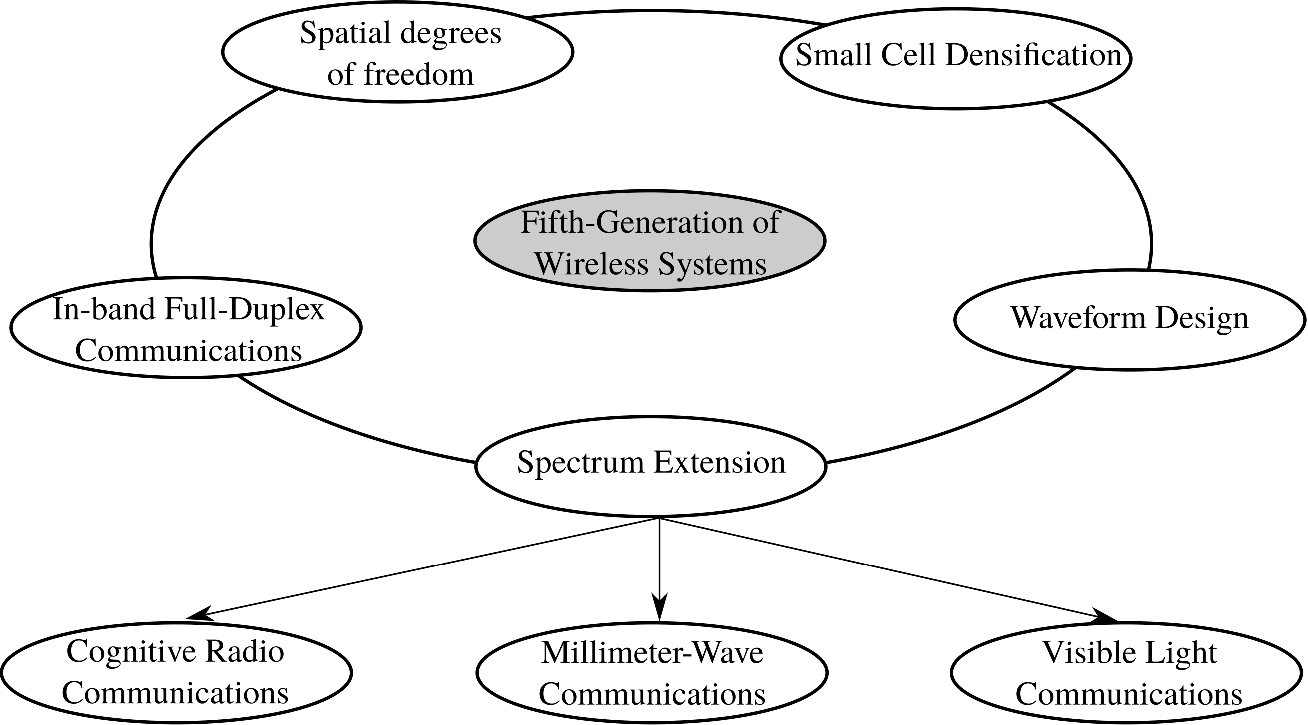
\includegraphics[width = 0.75\columnwidth]{figures/5G.ps}
        	};	
		%\node[draw = none,align=center] (A) at (0.23,0.53) {> \SI{6}{GHz}};
		\only<1>
		{
		\draw[decorate, decoration={brace, amplitude=10pt}, xshift = -4pt, yshift=0pt] (0.0,-0.7) -- (2.8,-0.7) node[black,midway,yshift=+0.5cm] {< \SI{6}{GHz}};
		\draw[decorate, decoration={brace, amplitude=10pt}, xshift = -4pt, yshift=0pt] (3.15,-0.7) -- (5.95,-0.7) node[black,midway,yshift=+0.5cm] {\SI{6}{GHz} -- \SI{300}{GHz}};
		\draw[decorate, decoration={brace, amplitude=10pt}, xshift = -4pt, yshift=0pt] (6.3,-0.7) -- (9.1,-0.7) node[black,midway,yshift=+0.5cm] {\SI{430}{THz} -- \SI{770}{THz}};
		%\draw[-latex] (B) edge (A);
		}
		\only<1>
		{
			\fill[opacity = 0.4, fill = kit-green30] (-0.1,-0.4) rectangle (8.9,2.2);
		}
		\only<2>
		{
			\fill[opacity = 0.4, fill = kit-green30] (-0.1,-0.4) rectangle (2.7,1.15);
			\fill[opacity = 0.4, fill = kit-green30] (3.0,-0.4) rectangle (8.9,1.15);
		}	
		\only<3->
		{
			\draw[opacity = 0, decorate, decoration={brace, amplitude=10pt}, xshift = -4pt, yshift=0pt] (0.0,-0.7) -- (2.8,-0.7) node[black,midway,yshift=+0.5cm] {< \SI{6}{GHz}};
			\draw[opacity = 0, decorate, decoration={brace, amplitude=10pt}, xshift = -4pt, yshift=0pt] (3.15,-0.7) -- (5.95,-0.7) node[black,midway,yshift=+0.5cm] {\SI{6}{GHz} -- \SI{300}{GHz}};
			\draw[opacity = 0.0, decorate, decoration={brace, amplitude=10pt}, xshift = -4pt, yshift=0pt] (6.3,-0.7) -- (9.1,-0.7) node[black,midway,yshift=+0.5cm] {\SI{430}{THz} -- \SI{770}{THz}};
			\fill[opacity = 0.4, fill = kit-green30] (-0.1,-0.4) rectangle (2.7,1.15);
			\fill[opacity = 0.0, fill = kit-green30] (3.0,-0.4) rectangle (8.9,1.15);
		}
		\end{tikzpicture}
	\end{center}
	\end{overlayarea}
	\begin{center}
		\only<1>
		{
			\tikzfancyarrow[11.0cm][kit-green70][top color=kit-green30, bottom color=kit-green50, shape border rotate=0]{Electromagnetic Spectrum}
		}
		\only<2>
		{
			\tikzfancyarrow[11.0cm][kit-green70][top color=kit-green30, bottom color=kit-green50, shape border rotate=180]{Mobility}
		}
		\only<3>
		{
			\begin{block}{}
			A Cognitive Radio (CR) is an agile system that facilitates an efficient usage (secondary access) of the spectrum below $\SI{6}{GHz}$ 
			\end{block}
		}
	\end{center}


\end{frame}


\subsection{Cognitive Small Cell}
%%%%%%%%%%%%%%%%%%%%%%%%%%%%%%%%%%%%%%%%%%%%%%%%%%%%%%%%%%%%%%%%%%%%%%%%%%%%%%%%
\begin{frame}[t]{Cognitive Small Cell}
%%%%%%%%%%%%%%%%%%%%%%%%%%%%%%%%%%%%%%%%%%%%%%%%%%%%%%%%%%%%%%%%%%%%%%%%%%%%%%%%
\pnote{A comprehensive incorporation of CR system in a preliminary 5G architecture in the form of CSC is illustrated.} 
\pnote{A CSC is a network entity that enable CR communications for the devices operating indoor.}
\pnote{In order to enhance the viability of the proposed architecture, some essential ingredients are highlighted}
\pnote{The architecture presented comprises of following network elements, MC-BS, MSs as a part of the CSC and MC, CSC-BS.}
\pnote{Next, different spectrum access schemes, pertaining to proposed 5G architecture, are presented. Wireless backhaul link represents a link between MC-BS and CSC-BS (representing a control and data plane). Following the trends, the mm-Wave, visible light communications and exclusively acquired spectrum are the potential candidates in support of wireless backhaul communications.}
\pnote{Direct link corresponds to the conventional link that already exist between the MC-BS and MS. The spectrum for the direct access correspond to conventional link.} 
\pnote{Indirect link corresponds to the CR communications, a spectrum is acquired for secondary usage is utilized for indoor communications.} 
\pnote{Next, it is worthy to understand that why an indoor deployment is proposed for disposition of CR techniques. From a market survey, it has been revealed that 70\% of the data traffic is originated indoor, thus by deploying CSC one attempts to consolidate these traffic sources. Besides, the indoor deployment provides a spatial separation between licensed and unlicensed users.} 
%Question: Regarding the Please note that the presented architecture in the dissertation is currently in a preliminary format. This can be extended further from a conceptual viewpoint.  
		\vspace{-0.3cm}
		\fs{7}{8}
		\begin{block}{}%{\scriptsize Cognitive Small Cell?}
		An Cognitive Small Cell (CSC) is a network entity that enable CR communications for the devices operating indoor 
		\end{block}
	\begin{columns}
	\begin{column}{0.37\columnwidth}
		\vspace{-0.1cm}
		\onslide<2->
		{	
			\begin{block}{\scriptsize Network Elements}
				\begin{itemize}
					\item Cognitive Small Cell-Base Station ($\color{blue}{\text{CSC-BS}}$)
					\item Mobile Station ($\color{kit-green100}{\text{MS}}$) 
					\item Macro Cell-Base Station ($\color{red}{\text{MC-BS}}$) 
				\end{itemize}
			\end{block}
		}
		\onslide<3->
		{
			\begin{block}{\scriptsize Spectrum Access}
				\begin{itemize}
					\item Wireless backhaul link ($\color{blue}{\text{CSC-BS} \Leftrightarrow \text{MC-BS}}$)
					\item Direct link ($\color{kit-green100}{\text{MC-BS} \Leftrightarrow \text{MS}}$) 
					\item Indirect link ($\color{red}{\text{CSC-BS} \Leftrightarrow \text{MS}}$) 
				\end{itemize}
			\end{block}
		}
		\onslide<4->
		{
			\begin{block}{\scriptsize Indoor?}
				\begin{itemize}
					\item 70\% traffic is originated indoor $\Leftrightarrow$ Traffic Management
					\item Spatial separation $\Leftrightarrow$ Interference suppression	
				\end{itemize}
			\end{block}
		}
	\end{column}
	\begin{column}{0.63\columnwidth}
		\fs{7}{8}
		\begin{center}
			CSC in a preliminary 5G network \\\vspace{0.4cm} 
        		\begin{tikzpicture}[scale=1]
				\node[anchor=south west,inner sep=0] (image) at (0,0)
				{
					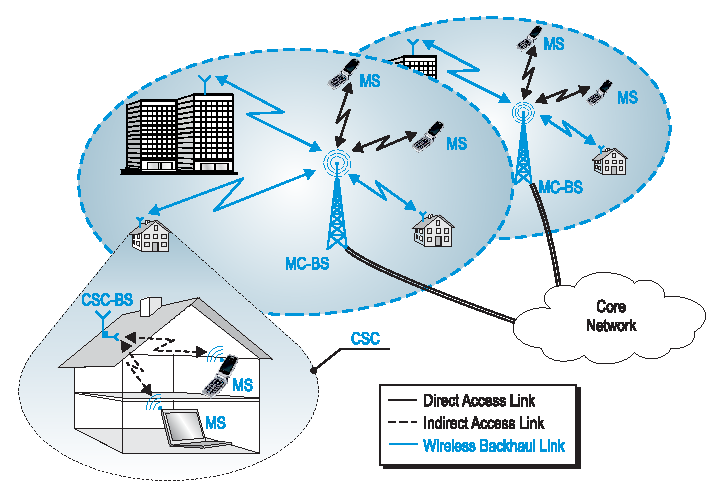
\includegraphics[width = \columnwidth]{../kapitel01/figures/Cellular_Scenario_CR6F}	     
				};
				\only<2>
				{
					\fill[opacity = 0.2, fill = blue] (0.65,1.47) rectangle (1.28,2.03);
					\fill[opacity = 0.2, fill = kit-green100] (1.5,.33) rectangle (2.32,.81);
					\fill[opacity = 0.2, fill = red] (2.8,2.2) rectangle (3.59,3.57);
				}
				\only<3>
				{
					\fill[opacity = 0.2, fill = blue] (1.37,2.78) rectangle (3.2,3.35);
					\fill[opacity = 0.2, fill = kit-green100] (3.35,3.5) rectangle (3.6,4.3);
					\fill[opacity = 0.2, fill = red] (1.08,0.89) rectangle (2.05,1.61);
				}
			\end{tikzpicture}	
		\end{center}
	\end{column}
	\end{columns}
\end{frame}

\subsection{Performance Analysis}
%%%%%%%%%%%%%%%%%%%%%%%%%%%%%%%%%%%%%%%%%%%%%%%%%%%%%%%%%%%%%%%%%%%%%%%%%%%%%%%%
\begin{frame}[t]{Performance Analysis of CR System}
%%%%%%%%%%%%%%%%%%%%%%%%%%%%%%%%%%%%%%%%%%%%%%%%%%%%%%%%%%%%%%%%%%%%%%%%%%%%%%%%
\pnote{Performance analysis in context to wireless system has two main objectives: Firstly, It help us understand the feasibility of a wireless system in real or close to real conditions. Secondly, it allows us to determine the performance limits.} 
\pnote{Coexistence of different wireless systems (refer to the figure and highlight the primary and secondary system) has always been a difficult task, the task becomes even more challenging if we take into account the fact that two different system (which may differ in their communication standards) coexists, i.e., share a band of spectrum, separated in time, space or polarization.}
\pnote{From a physical layer perspective, with no concrete guidelines (although there exists certain use cases, but are applicable to specific specific scenarios) available on how to choose the primary user signal. As a result, only solutions will persist that consider no knowledge of primary user signals, for instance energy detection. In other words, versatile and applicable to large range of wireless system.}  
\pnote{It is well-know fact that concept of CR has been under discussion over the last 18 years, during this time line several models have been established, characterizing the performance of CR systems. However, due to the complexity of the underlaying scenario, very few are models have been implemented over the hardware. Leaving their performance analysis questionable.}
\pnote{Since we are dealing with two different systems, it is important to jointly quantify their performance. From a physical layer perspective, secondary access to the licensed spectrum can be made possible through the application of CR techniques at the ST. In order to coexist, a CR system guarantee a sufficient protection to the primary system in the form of interference power received at the PR.}
\pnote{On the other end, in order to co-benefit from the secondary access, the CR system guarantees a certain QoE in the form of throughput at the SR} 
\pnote{It is been determined that the performance characterization as-well-as for the feasibility of CR techniques require the knowledge of involved channels. } 
	\vspace{-3mm}
	\fs{7}{8}
	\begin{block}{\scriptsize Challenges}
		\begin{itemize}
			\item Involves the coexistence of two different system: {\color{blue}{primary}} and {\color{red}{secondary}} 
			\item Lack of concrete guidelines available in the literature $\Rightarrow$ only those solutions persist that consider no knowledge about the primary user signal 
			% With regard to the above issues 
			\item Existing theoretical analysis rarely converges to a hardware implementation $\Rightarrow$ deployment perspective % in order words, rarely deal(tackle) the problem from a deployment perspective 
		\end{itemize}
	\end{block}
	\vspace{-1mm}
	\begin{columns}
		\begin{column}{0.37\columnwidth}
			\onslide<2->
			{
				\begin{block}{\scriptsize Performance characterization}
					Upon applying CR techniques at ST, a CR system guarantees\begin{itemize}
						\item Protection to primary system $\Leftrightarrow$ interference power at PR 
						\item QoE to secondary system $\Leftrightarrow$ at SR 
					\end{itemize}
				\end{block}
			}
			\vspace{-1mm}
			\onslide<3->
			{
				\begin{block}{}%{\scriptsize Channel knowledge}
					Knowledge of interacting channels is absolutely necessary at ST 
				\end{block}
			}
			\onslide<4->
	 		{
				\centering
				\tikzfancyarrow[0.85cm][kit-green70][top color=kit-green50, bottom color=kit-green50, shape border rotate=270]{\color{kit-green50}{10}}			\\[0.5em]	
	               		\begin{tikzpicture}[scale=1]
	               	 		\node[draw=none,fill=kit-green15, minimum height = 0.5cm, text width = \columnwidth, align = center] at (0.0, 0.0) {Channel Estimation is proposed at ST/SR};
				\end{tikzpicture}
			}
		\end{column}
		\begin{column}{0.63\columnwidth}
		\vspace{-1mm}
		\fs{7}{8}
		\begin{center}
			% Interacting entities
			{\color{blue}{PT, PR}}, \color{red}{ST($\Leftrightarrow$ CSC-BS) and SR($\Leftrightarrow$ MS)}\\\vspace{0.2cm} 
        		\begin{tikzpicture}[scale=1]
				\node[anchor=south west,inner sep=0] (image) at (0,0)
				{
					\includegraphics[width = 0.85\columnwidth]{../kapitel01/figures/CR_Scenario_Hybrid}	     
				};
				\only<1>
				{
					\fill[opacity = 0.2, fill = blue] (.32,1.16) rectangle (1.22,1.8);
					\fill[opacity = 0.2, fill = blue] (.32,-0.06) rectangle (1.22,0.58);
					\fill[opacity = 0.2, fill = red] (3.65,1.18) rectangle (4.65,1.6);
					\fill[opacity = 0.2, fill = red] (2.42,2.3) rectangle (3.88,3.08);
				}
				\only<2>
				{
					\draw[blue, thick] (.32,1.16) rectangle (1.22,1.8); %PR
					\draw[red, thick] (3.65,1.18) rectangle (4.65,1.6); %ST
					\draw[red, thick] (2.42,2.3) rectangle (3.88,3.08); %SR
					
					%% Dummy figure added to avoid a shift between two slides
					\fill[opacity = 0.0, fill = blue] (.32,-0.06) rectangle (1.22,0.58);
				}
				\only<3->
				{
					
					\fill[opacity = 0.2, fill = kit-green100] (1.28,.98) rectangle (1.68,1.34);
					\fill[opacity = 0.2, fill = kit-green100] (1.22,1.96) rectangle (1.62,2.32);
					\fill[opacity = 0.2, fill = kit-green100] (3.38,1.86) rectangle (3.78,2.22);
					\fill[opacity = 0.2, fill = kit-green100] (2.52,.68) rectangle (2.92,1.04);
					
					%% Dummy figure added to avoid a shift between two slides
					\fill[opacity = 0.0, fill = blue] (.32,-0.06) rectangle (1.22,0.58);
				}
				\only<4->
				{
					\draw[red, thick] (3.65,1.18) rectangle (4.65,1.6); %ST
					\draw[red, thick] (2.42,2.3) rectangle (3.88,3.08); %SR
				}
			\end{tikzpicture}	
		\end{center}
		\end{column}
	\end{columns}
\end{frame}


%%%%%%%%%%%%%%%%%%%%%%%%%%%%%%%%%%%%%%%%%%%%%%%%%%%%%%%%%%%%%%%%%%%%%%%%%%%%%%%%
\begin{frame}[t]{Major Contributions}
%%%%%%%%%%%%%%%%%%%%%%%%%%%%%%%%%%%%%%%%%%%%%%%%%%%%%%%%%%%%%%%%%%%%%%%%%%%%%%%%
	\pnote{The major contributions are summarized as follows:}
	\pnote{From a system design's perspective, it is important to accommodate the channel estimation into the system model. Hence, the system has cope up with the variations induced in the system due to imperfect channel knowledge, at the same time allocate resources for channel estimation}
	\pnote{These variations are captured by means of a stochastic model. Furthermore, a certain amount of time resources are allocated for channel estimation in the secondary user frame structure.} 
	\pnote{With regard to the psychology established in the previous slide, with no knowledge of the primary user signals, we are faced with the challenge of estimating the channels that exists between two different systems. With this situation in hand, conventional estimation techniques are not applicable. Besides, we have to look for techniques that offer versatility towards unknown primary user signals and low complexity.}
	\pnote{ In this regard, a novel estimation technique termed as received-power based estimation is proposed that satisfies the low-complexity and versatility requirements.}
	\pnote{It is an obvious fact that channel estimation will certainly has a detrimental effect on the performance, thereby degrading the performance of CR systems, in terms of uncertainty in the interference caused due to imperfect channel knowledge or variations induced in the system. Secondly, degradation in throughput caused due to the time allocation.} 
	\pnote{In order to regulate uncertainty in interference, new interference constraints are proposed. Secondly, the interplay between the uncertain interference and the secondary throughput is analyzed in terms of performance tradeoffs. These tradeoffs allow us to determine the suitable estimation time that yields the maximum throughput achieved by the CR systems.}
	\pnote{In order to verify the propositions made while establishing the system model, a hardware is deployed using a software-defined platform.}
	\pnote{Finally, a applicability of the proposed framework in realistic conditions is presented by means of a hardware demonstrator}  
	\vspace{-1.5mm}
	\begin{columns}
		\begin{column}[t]{0.53\columnwidth}
			\centering Challenges: \\[-0.2em]
				\fs{7}{8}
				\begin{block}{\scriptsize System design aspects?} %of incorporating channel estimation on the performance
					\begin{itemize} 
						\item How to tackle the variations induced? 
						\item Time allocation for channel estimation 
						%\item Channel fading 
					\end{itemize}
				\end{block}
				\vspace{-1.1mm}
				\onslide<2->
				{
				\begin{block}{\scriptsize Estimation technique?} %{\scriptsize Challenges}
					Estimation of channels between two different systems %$\Rightarrow$ 
					\begin{itemize}
						\item Conventional techniques are not feasible  
						\item Complexity and versatility towards unknown primary user signals
					\end{itemize}
				\end{block}
				}
				\vspace{-1.1mm}
				\onslide<3->
				{
				\begin{block}{\scriptsize Impact on performance?}%{\scriptsize Channel knowledge}
					\begin{itemize}
						\item Primary system $\Rightarrow$ uncertain interference 
						\item Secondary system $\Rightarrow$ degradation in throughput 
					\end{itemize} 
				\end{block}
				}	
				\vspace{-1.1mm}
				\onslide<4->
				{
				\begin{block}{\scriptsize Hardware Feasibility?}%{\scriptsize Channel knowledge}
					\begin{itemize}
					\item Validity of the propositions made? 
					\item Applicability of the proposed framework under realistic scenarios? 
					\end{itemize}	
				\end{block}
				}
		\end{column}
		
		\begin{column}{0.03\columnwidth}
		\end{column}
		
		\begin{column}[t]{0.44\columnwidth}
			\centering Proposed Solutions: \\[-0.2em]
			\fs{7}{8}
			\begin{block}{}
				\centering
			  	Stochastic modeling \\ To characterize the variations 	
			\end{block}
			\vspace{-0.5mm}
			\begin{block}{}
				\centering
			   	Time allocation for channel estimation in secondary user's frame structure
			\end{block}
			\vspace{-0.5mm}
			\onslide<2->
			{
			\begin{block}{}
				\centering
				Received power based channel estimation
				%\begin{itemize}
					%\item 
					Low-complexity and versatility requirements are satisfied  
					%\item Incorporation of received power in performance characterization 
				%\end{itemize}
			\end{block}
			}
			\vspace{-0.5mm}
			\onslide<3->
			{
			\begin{block}{}
				\centering
			  	Interference constraints  \\To protect PR from harmful interference 
			\end{block}
			}	
			\vspace{-0.5mm}
			\onslide<3->
			{
			\begin{block}{}
				\centering
			 	Performance tradeoffs \\ To determine suitable estimation time that determines the achievable throughput	
			\end{block}
			}
			\vspace{-0.4mm}
			\onslide<4->
			{
			\begin{block}{}%{\scriptsize Hardware Feasibility}%{\scriptsize Channel knowledge}			
				\centering
				Empirical validation \\ Hardware demonstration
				%\begin{itemize}
					%\item Empirical validation %of the derived expressions
					%\item Hardware demonstration %of a CR system
				%\end{itemize}	
			\end{block}
			}
		\end{column}
	\end{columns}
\end{frame}

%%%%%%%%%%%%%%%%%%%%%%%%%%%%%%%%%%%%%%%%%%%%%%%%%%%%%%%%%%%%%%%%%%%%%%%%%%%%%%%%%
%\begin{frame}[c]{Contributions}
%%%%%%%%%%%%%%%%%%%%%%%%%%%%%%%%%%%%%%%%%%%%%%%%%%%%%%%%%%%%%%%%%%%%%%%%%%%%%%%%%
%	\vspace{-2mm}
%	%\hspace{-2mm}
%	\begin{center}
%	\begin{tikzpicture}[scale=1]
%                                \node[anchor=south west,inner sep=0] (image) at (0,0)
%                                {
%                                        \includegraphics[width = 1.0\columnwidth]{../kapitel01/figures/Contri.ps}
%                                };
%                        \end{tikzpicture}
%	\end{center}
%\end{frame}

\fi

\ifinter
\section{Interweave System}
%%%%%%%%%%%%%%%%%%%%%%%%%%%%%%%%%%%%%%%%%%%%%%%%%%%%%%%%%%%%%%%%%%%%%%%%%%%%%%%%
\begin{frame}[c]{}
%%%%%%%%%%%%%%%%%%%%%%%%%%%%%%%%%%%%%%%%%%%%%%%%%%%%%%%%%%%%%%%%%%%%%%%%%%%%%%%%
\begin{center}
Interweave System
\end{center}
\end{frame}

%%%%%%%%%%%%%%%%%%%%%%%%%%%%%%%%%%%%%%%%%%%%%%%%%%%%%%%%%%%%%%%%%%%%%%%%%%%%%%%%
\begin{frame}[t]{Interweave System}
%%%%%%%%%%%%%%%%%%%%%%%%%%%%%%%%%%%%%%%%%%%%%%%%%%%%%%%%%%%%%%%%%%%%%%%%%%%%%%%%
	\pnote{Here the deployment scenario corresponding to CSC is transformed into an interweave system}
	\pnote{Spectrum sensing, a CR technique, is employed at the ST}
	\pnote{In this way, by listening to signal transmitted by the PT, the ST protects the PR, by not transmitting its own signal whenever the primary user signal is detected.} 
	\pnote{Corresponding to this approach the following signal model is proposed. The signal received at the ST over the channel $\hpo$ depends on the following hypothesis, the PT is active and PT is inactive}
	\pnote{The signal is received at the SR only under two conditions, wherever there is a misdetection or the condition where no false alarm happens.} 
	\pnote{With reference to the signal model, the performance of the CR system can be jointly characterized in terms of detectors performance, which symbolizes the primary system performance and throughput received at SR}
	\pnote{The detector's performance can be characterized in terms of the detection probability and false alarm probability. Considering the fact that no knowledge concerning the PU signal is available, energy detectors is employed.}
	\pnote{Secondary throughput, corresponding to the signal model, the signal received at SR is with and without interference from PT. The prefactor corresponds to the time resources allocated for sensing.} 
	\pnote{It is worthy to point out that the characterization of the performance parameters requires the knowledge of the involved channels} 
	\vspace{-2mm}
	\fs{7}{8}
	\begin{columns}
		\begin{column}{0.44\columnwidth}
				%\vspace{-1mm}
			\begin{block}{\scriptsize Principle} %{\scriptsize Principle}
				\begin{itemize}
					\item Interweave system employs spectrum sensing at the ST 
					\item Spectrum sensing is CR technique used for detecting the signals transmitted by PT
					%\item Energy detector is employed 
				\end{itemize}
			\end{block}
			\vspace{-1mm}
			\onslide<2->
			{
				\begin{block}{\scriptsize Signal model} %{\scriptsize Signal model}
				\begin{equation*}
					\yrcvd[n] = 
					\begin{cases}
					\hpo \cdot \xp[n] + \wst[n] & : \mathcal{H}_1 \\
					\wst[n] & :\mathcal{H}_0
					\end{cases}
					%\label{eq_IS:sys_mod_p1s}
				\end{equation*}
				\begin{equation*}
					\ys[n] = 
					\begin{cases}
						\hs \cdot \xs[n] + \hpt \cdot \xp[n] +  \wsr[n] & \\%: 1 - \pd \\
						\hs \cdot \xs[n] + \wsr[n] & %: 1 - \pfa
					\end{cases}
					\label{eq_IS:sys_mod_ss}
				\end{equation*}
				\end{block}
			}
			\onslide<3->
			{
			
				\vspace{-1mm}
				\begin{block}{\scriptsize Energy detector's performance} %Detector performance Interference at PR is dependent on the detectors performance
				\begin{equation*}
						\pd = \Gamma\left( \frac{\tsen \fsam}{2}, \frac{\tsen \fsam \mu}{2 \color{kit-green100}{\prcvdstpt}} \right), %\\ 
				\end{equation*}	
				\begin{equation*}
						\pfa = \Gamma\left( \frac{\tsen \fsam}{2}, \frac{\tsen \fsam \mu}{2 \npo} \right)%,  \label{eq_IS:pfa} 
				\end{equation*}	
				\end{block}	
			}
		\end{column}
		\begin{column}{0.56\columnwidth}
		\vspace{6mm}
		\fs{7}{8}
		\begin{center}
			% Interacting entities
			%Interweave Scenario \\\vspace{0.2cm} 
        		\begin{tikzpicture}[scale=1]
				\node[anchor=south west,inner sep=0] (image) at (0,0)
				{
					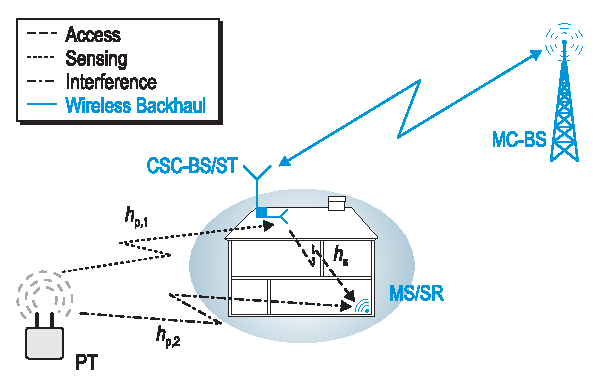
\includegraphics[width = 0.9\columnwidth]{../kapitel03/figures/CR_Scenario_Interweave}	     
				};
				\only<3>
				{
					\fill[opacity = 0.2, fill = kit-green100] (1.03,1.41) rectangle (1.43,1.75);
					\fill[opacity = 0.2, fill = kit-green100] (1.35,0.2) rectangle (1.75,.54);
					\fill[opacity = 0.2, fill = kit-green100] (3.13,0.98) rectangle (3.53,1.34);
				}
			\end{tikzpicture}	
		\end{center}
		\onslide<3->	
		{\begin{block}{\scriptsize Secondary throughput} %Secondary throughput
                                \vspace{-2.6mm}
				\begin{align*}
                               		\rs(\tsen) =& \frac{T- \tsen}{T} \bigg[ \log_2 \left(1 + {\color{kit-green100}{|\hs|^2}} \frac{\ptranst}{\npo}\right) (1 - \pfa) \phz  \\ & + \log_2 \left(1 + \frac{{\color{kit-green100}{|\hs|^2}} \ptranst }{{\color{kit-green100}{|\hpt|^2}} \ptranpt  + \npo } \right)  (1 - \pd) \pho  \bigg] 
				\end{align*} 
                \end{block} 	
		}
		\end{column}
	\end{columns}
\end{frame}

%%%%%%%%%%%%%%%%%%%%%%%%%%%%%%%%%%%%%%%%%%%%%%%%%%%%%%%%%%%%%%%%%%%%%%%%%%%%%%%%
\begin{frame}[t]{Interweave System}
%%%%%%%%%%%%%%%%%%%%%%%%%%%%%%%%%%%%%%%%%%%%%%%%%%%%%%%%%%%%%%%%%%%%%%%%%%%%%%%%
	\pnote{In an idealistic scenario that assumes the knowledge of the involved channels, it is possible to determine a suitable sensing time that achieves a maximum throughput such that detection probability mainly responsible for causing interference is constrained}
	\pnote{It is worthy to that since no knowledge regarding the channels is available, such an optimization yields inadequate results}
	\pnote{To resolve this issue, following approach is proposed, the time resources are allocated at the ST and the SR frame structure.}
        \pnote{The variations due to the estimation of the involved channels are characterized in terms of their cdf.}
	\pnote{It is worthy to mention here that the received power estimation is employed for the channels between the primary and secondary systems and pilot based estimation is employed for the channel within the secondary system} % In this regard, the estimated parameters is observed indirectly in the form of received power 
	\pnote{Next, the variations in the performance parameters are characterized using their cdfs, where C0 and C1 corresponds to the data rate with and without interference in the throughput expression}
	\pnote{The cdfs of the performance parameters are used to determine the suitable estimation and sensing time intervals that achieves the maximum secondary throughput.}
	\pnote{Based on the proposed approach, an estimation model that include channel estimation that yields the achievable throughput while satisfying the new interference constraints on the detection probability}
	\pnote{In this work, an average and outage constraint is proposed.} 
	\vspace{-2mm}
	\fs{7}{8}
	%\begin{block}{}
	%\end{block}			
	\begin{columns}
		\begin{column}{0.38\columnwidth}
			%\vspace{-1mm}
			\begin{block}{\scriptsize Ideal Model (IM)}
     			   	\vspace{-4.5mm}
	    		        \begin{align*}
				\trs(\ttsen) =& \maxi_{\tsen} \trs(\tsen)\\ 
				\text{s.t.} & \text{ } \pd \ge \pdd	
	        	\end{align*}
			%Without the knowledge of channel gains $\phpo$, $\phpt$ and $\phs$, it is difficult to characterize the performance parameters $\pd$ and $\rs$  
			\end{block}
			\vspace{-1.5mm}
			\begin{block}{\scriptsize Proposed Approach}
			\begin{center}
			\begin{tikzpicture}[node distance = 1.27cm, auto]
                        	% draw nodes
				\node [block] (frame) {Incorporation of time resources for channel estimation and sensing in frame structure ($\test, \tsen$)};
  			        \node [block, below of=frame] (channelest) {Variations due to channel estimation ($\pgpo$, $\pgpt$, $\pgs$) are characterized in terms of $\fprcvd, \fprcvdsr, \fpgpt$};
  			        \node [block, below of=channelest] (cdf) {Variations in performance parameters ($\epd$, $\ecz$, $\eco$) are characterized in terms of $\fpd, \fcz, \fco$};
  			        \node [block, below of=cdf] (tradeoff) {The cdfs are used to determine the achievable secondary throughput subject to interference constraints};
				% draw edges
    				\path [line] (frame) -- (channelest);
    				\path [line] (channelest) -- (cdf);
    				\path [line] (cdf) -- (tradeoff);
			\end{tikzpicture}
			\end{center}
			\end{block}

		\end{column}
		\begin{column}{0.62\columnwidth}
		\fs{7}{8}
		\begin{center}
        		%Frame Structure \\\vspace{2mm}
			\begin{overlayarea}{\textwidth}{4.1cm}
			\begin{tikzpicture}[scale=1]
				\node[anchor=south west,inner sep=0] (image) at (0,0)
				{
					\includegraphics[width = \columnwidth]{figures/Frame_Structure_IS.ps}     
				};
				\fill[opacity = 0.4, fill = kit-green100] (0.84,1.35) rectangle (1.55,1.71);
				\fill[opacity = 0.4, fill = kit-green100] (4.01,1.35) rectangle (4.72,1.71);
				\fill[opacity = 0.4, fill = kit-green100] (0.84,2.97) rectangle (1.55,3.33);
				\fill[opacity = 0.4, fill = kit-green100] (4.01,2.97) rectangle (4.72,3.33);
			\end{tikzpicture}	
                        \end{overlayarea}
			\vspace{3.5mm}
			\begin{overlayarea}{\textwidth}{2.6cm}
			\only<1>
			{	
				\begin{block}{\scriptsize Estimation Model (EM) -- Average Constraint (AC)} 
                               	 \vspace{-3.2mm}
					\begin{align*}
					\trsac(\ttest, \ttsenac) =& \maxi_{\test, \tsen} \e{\epd, \ecz, \eco}{\rs(\test, \tsen)},	\\	
					\text{s.t.} & \text{ }  \color{kit-green100}{\e{\epd}{\epd} \ge \pdd}, \\ 
\text{s.t.} & \text{ }  0 < \test \le \tsen \le T
					\end{align*} 
               		 	\end{block}
			} 
			\only<2->
			{	
				\begin{block}{\scriptsize Estimation Model (EM) -- Outage Constraint (OC)} 
                               	 \vspace{-3.2mm}
					\begin{align*}
					\trsac(\ttest, \ttsenac) =& \maxi_{\test, \tsen} \e{\epd, \ecz, \eco}{\rs(\test, \tsen)},	\\	
					\text{s.t.} & \text{ }  \color{kit-green100}{\p(\epd \le \pdd) \le \mpd}, \\[0.35em]
\text{s.t.} & \text{ }  0 < \test \le \tsen \le T
					\end{align*} 
               		 	\end{block}
			} 
                        \end{overlayarea}
		\end{center}
		\end{column}
	\end{columns}
\end{frame}


%%%%%%%%%%%%%%%%%%%%%%%%%%%%%%%%%%%%%%%%%%%%%%%%%%%%%%%%%%%%%%%%%%%%%%%%%%%%%%%%
\begin{frame}[t]{Interweave System}
%%%%%%%%%%%%%%%%%%%%%%%%%%%%%%%%%%%%%%%%%%%%%%%%%%%%%%%%%%%%%%%%%%%%%%%%%%%%%%%%
	\pnote{It is worthy to mention here that theoretical expressions are derived in the thesis are used for performance analysis, these expressions are verified by means of Monte Carlo simulation}
	\pnote{A glimpse of the parameters used for performance analysis}
	\pnote{Sampling frequency, Channel gain, frame duration, noise power, occurrence probability, Number of pilot symbols used for pilot-based channel estimation.}
	\pnote{Here, we analyze the variation of secondary throughput along the estimation for idealistic approach and estimation model in reference to average and outage constraint.} 
	\pnote{An ideal model is used for evaluating the performance degradation acquired due to incorporation of channel knowledge}
	\pnote{The figure depicts a tradeoff between a tradeoff between the estimation and secondary throughput. Based on this analysis it is revealed that performance degradation can be effectively regulated by choosing the estimation time appropriately} % The estimation time 
	\pnote{The analysis clearly reveals that the OC presenting an aggressive way of tacking the variations results in large degradation in performance.}
 
	\vspace{-2mm}
	\begin{columns}
	\begin{column}{0.45\columnwidth}
	\fs{7}{8}
		\renewcommand{\arraystretch}{1.55}
		\begin{tabular}{c||c}
		%\hline
		\rowcolor{kit-green30}
		Parameter & Value \\
		\hline\hline
		$\fsam$ & $\SI{1}{MHz}$ \\ %\hline
		$\phpo$ & $\SI{-100}{dB}$ \\ %\hline
		$\phpt$ & $\SI{-100}{dB}$ \\ %\hline
		$\phs$ & $\SI{-80}{dB}$ \\ %\hline 
		$T$ & $\SI{100}{ms}$ \\ %\hline 
		$\npo$ & $\SI{-100}{dBm}$ \\ %\hline
		$\snrrcvd$ & $\SI{-10}{dB}$ \\ %\hline
		$\snrpt$ & $\SI{-10}{dB}$ \\ %\hline
		$\snrso$ & $\SI{10}{dB}$ \\ %\hline
		%$\ptranpt$ & $-\SI{10}{dBm}$ \\ %\hline
		%$\ptranst$ & $-\SI{10}{dBm}$ \\ %\hline
		$\pho = 1 - \phz$ & 0.2 \\ %\hline
		%$\test$ & $\SI{5}{ms}$ \\ %\hline
		$\Ks$ & 10 \\ \hline
		%$\Kp$ & $1000$ \\ \hline
	\end{tabular}

	\end{column}
	\begin{column}{0.55\columnwidth}
	\begin{center}
	\fs{7}{8}	
		%% Add psfrag entries
		% This file is generated by the MATLAB m-file laprint.m. It can be included
% into LaTeX documents using the packages graphicx, color and psfrag.
% It is accompanied by a postscript file. A sample LaTeX file is:
%    \documentclass{article}\usepackage{graphicx,color,psfrag}
%    \begin{document}% This file is generated by the MATLAB m-file laprint.m. It can be included
% into LaTeX documents using the packages graphicx, color and psfrag.
% It is accompanied by a postscript file. A sample LaTeX file is:
%    \documentclass{article}\usepackage{graphicx,color,psfrag}
%    \begin{document}% This file is generated by the MATLAB m-file laprint.m. It can be included
% into LaTeX documents using the packages graphicx, color and psfrag.
% It is accompanied by a postscript file. A sample LaTeX file is:
%    \documentclass{article}\usepackage{graphicx,color,psfrag}
%    \begin{document}\input{fig_opt_thr_vs_est_time_diff_mu_AWGN}\end{document}
% See http://www.mathworks.de/matlabcentral/fileexchange/loadFile.do?objectId=4638
% for recent versions of laprint.m.
%
% created by:           LaPrint version 3.16 (13.9.2004)
% created on:           12-Jul-2016 15:03:36
% eps bounding box:     16 cm x 12 cm
% comment:              
%
%\begin{psfrags}%
%\psfragscanon%
%
% text strings:
\psfrag{s05}[b][b]{\fontsize{8}{12}\fontseries{m}\mathversion{normal}\fontshape{n}\selectfont \color[rgb]{0,0,0}\setlength{\tabcolsep}{0pt}\begin{tabular}{c}$\trs(\test,\ttsen)$ [bits/sec/Hz]\end{tabular}}%
\psfrag{s06}[t][t]{\fontsize{8}{12}\fontseries{m}\mathversion{normal}\fontshape{n}\selectfont \color[rgb]{0,0,0}\setlength{\tabcolsep}{0pt}\begin{tabular}{c}$\test$ [ms]\end{tabular}}%
\psfrag{s10}[][]{\fontsize{10}{15}\fontseries{m}\mathversion{normal}\fontshape{n}\selectfont \color[rgb]{0,0,0}\setlength{\tabcolsep}{0pt}\begin{tabular}{c} \end{tabular}}%
\psfrag{s11}[][]{\fontsize{10}{15}\fontseries{m}\mathversion{normal}\fontshape{n}\selectfont \color[rgb]{0,0,0}\setlength{\tabcolsep}{0pt}\begin{tabular}{c} \end{tabular}}%
\psfrag{s12}[l][l]{\fontsize{8}{12}\fontseries{m}\mathversion{normal}\fontshape{n}\selectfont \color[rgb]{0,0,0}$\trs(\ttest,\ttsen)$}%
\psfrag{s13}[l][l]{\fontsize{8}{12}\fontseries{m}\mathversion{normal}\fontshape{n}\selectfont \color[rgb]{0,0,0}IM}%
\psfrag{s14}[l][l]{\fontsize{8}{12}\fontseries{m}\mathversion{normal}\fontshape{n}\selectfont \color[rgb]{0,0,0}EM-AC, Problem 1}%
\psfrag{s15}[l][l]{\fontsize{8}{12}\fontseries{m}\mathversion{normal}\fontshape{n}\selectfont \color[rgb]{0,0,0}EM-OC, Problem 2}%
\psfrag{s16}[l][l]{\fontsize{8}{12}\fontseries{m}\mathversion{normal}\fontshape{n}\selectfont \color[rgb]{0,0,0}Corollary 1}%
\psfrag{s17}[l][l]{\fontsize{8}{12}\fontseries{m}\mathversion{normal}\fontshape{n}\selectfont \color[rgb]{0,0,0}$\trs(\ttest,\ttsen)$}%
%
% axes font properties:
\fontsize{8}{12}\fontseries{m}\mathversion{normal}%
\fontshape{n}\selectfont%
%
% xticklabels:
\psfrag{x01}[t][t]{1}%
\psfrag{x02}[t][t]{2}%
\psfrag{x03}[t][t]{3}%
\psfrag{x04}[t][t]{4}%
\psfrag{x05}[t][t]{5}%
\psfrag{x06}[t][t]{6}%
\psfrag{x07}[t][t]{7}%
\psfrag{x08}[t][t]{8}%
\psfrag{x09}[t][t]{9}%
\psfrag{x10}[t][t]{10}%
%
% yticklabels:
\psfrag{v01}[r][r]{1.8}%
\psfrag{v02}[r][r]{1.9}%
\psfrag{v03}[r][r]{2}%
\psfrag{v04}[r][r]{2.1}%
\psfrag{v05}[r][r]{2.2}%
\psfrag{v06}[r][r]{2.3}%
\psfrag{v07}[r][r]{2.4}%
\psfrag{v08}[r][r]{2.5}%
\psfrag{v09}[r][r]{2.6}%
\psfrag{v10}[r][r]{2.7}%
%
% Figure:
%\resizebox{8cm}{!}{\includegraphics{fig_opt_thr_vs_est_time_diff_mu_AWGN.eps}}%
%\end{psfrags}%
%
% End fig_opt_thr_vs_est_time_diff_mu_AWGN.tex
\end{document}
% See http://www.mathworks.de/matlabcentral/fileexchange/loadFile.do?objectId=4638
% for recent versions of laprint.m.
%
% created by:           LaPrint version 3.16 (13.9.2004)
% created on:           12-Jul-2016 15:03:36
% eps bounding box:     16 cm x 12 cm
% comment:              
%
%\begin{psfrags}%
%\psfragscanon%
%
% text strings:
\psfrag{s05}[b][b]{\fontsize{8}{12}\fontseries{m}\mathversion{normal}\fontshape{n}\selectfont \color[rgb]{0,0,0}\setlength{\tabcolsep}{0pt}\begin{tabular}{c}$\trs(\test,\ttsen)$ [bits/sec/Hz]\end{tabular}}%
\psfrag{s06}[t][t]{\fontsize{8}{12}\fontseries{m}\mathversion{normal}\fontshape{n}\selectfont \color[rgb]{0,0,0}\setlength{\tabcolsep}{0pt}\begin{tabular}{c}$\test$ [ms]\end{tabular}}%
\psfrag{s10}[][]{\fontsize{10}{15}\fontseries{m}\mathversion{normal}\fontshape{n}\selectfont \color[rgb]{0,0,0}\setlength{\tabcolsep}{0pt}\begin{tabular}{c} \end{tabular}}%
\psfrag{s11}[][]{\fontsize{10}{15}\fontseries{m}\mathversion{normal}\fontshape{n}\selectfont \color[rgb]{0,0,0}\setlength{\tabcolsep}{0pt}\begin{tabular}{c} \end{tabular}}%
\psfrag{s12}[l][l]{\fontsize{8}{12}\fontseries{m}\mathversion{normal}\fontshape{n}\selectfont \color[rgb]{0,0,0}$\trs(\ttest,\ttsen)$}%
\psfrag{s13}[l][l]{\fontsize{8}{12}\fontseries{m}\mathversion{normal}\fontshape{n}\selectfont \color[rgb]{0,0,0}IM}%
\psfrag{s14}[l][l]{\fontsize{8}{12}\fontseries{m}\mathversion{normal}\fontshape{n}\selectfont \color[rgb]{0,0,0}EM-AC, Problem 1}%
\psfrag{s15}[l][l]{\fontsize{8}{12}\fontseries{m}\mathversion{normal}\fontshape{n}\selectfont \color[rgb]{0,0,0}EM-OC, Problem 2}%
\psfrag{s16}[l][l]{\fontsize{8}{12}\fontseries{m}\mathversion{normal}\fontshape{n}\selectfont \color[rgb]{0,0,0}Corollary 1}%
\psfrag{s17}[l][l]{\fontsize{8}{12}\fontseries{m}\mathversion{normal}\fontshape{n}\selectfont \color[rgb]{0,0,0}$\trs(\ttest,\ttsen)$}%
%
% axes font properties:
\fontsize{8}{12}\fontseries{m}\mathversion{normal}%
\fontshape{n}\selectfont%
%
% xticklabels:
\psfrag{x01}[t][t]{1}%
\psfrag{x02}[t][t]{2}%
\psfrag{x03}[t][t]{3}%
\psfrag{x04}[t][t]{4}%
\psfrag{x05}[t][t]{5}%
\psfrag{x06}[t][t]{6}%
\psfrag{x07}[t][t]{7}%
\psfrag{x08}[t][t]{8}%
\psfrag{x09}[t][t]{9}%
\psfrag{x10}[t][t]{10}%
%
% yticklabels:
\psfrag{v01}[r][r]{1.8}%
\psfrag{v02}[r][r]{1.9}%
\psfrag{v03}[r][r]{2}%
\psfrag{v04}[r][r]{2.1}%
\psfrag{v05}[r][r]{2.2}%
\psfrag{v06}[r][r]{2.3}%
\psfrag{v07}[r][r]{2.4}%
\psfrag{v08}[r][r]{2.5}%
\psfrag{v09}[r][r]{2.6}%
\psfrag{v10}[r][r]{2.7}%
%
% Figure:
%\resizebox{8cm}{!}{\includegraphics{fig_opt_thr_vs_est_time_diff_mu_AWGN.eps}}%
%\end{psfrags}%
%
% End fig_opt_thr_vs_est_time_diff_mu_AWGN.tex
\end{document}
% See http://www.mathworks.de/matlabcentral/fileexchange/loadFile.do?objectId=4638
% for recent versions of laprint.m.
%
% created by:           LaPrint version 3.16 (13.9.2004)
% created on:           12-Jul-2016 15:03:36
% eps bounding box:     16 cm x 12 cm
% comment:              
%
%\begin{psfrags}%
%\psfragscanon%
%
% text strings:
\psfrag{s05}[b][b]{\fontsize{8}{12}\fontseries{m}\mathversion{normal}\fontshape{n}\selectfont \color[rgb]{0,0,0}\setlength{\tabcolsep}{0pt}\begin{tabular}{c}$\trs(\test,\ttsen)$ [bits/sec/Hz]\end{tabular}}%
\psfrag{s06}[t][t]{\fontsize{8}{12}\fontseries{m}\mathversion{normal}\fontshape{n}\selectfont \color[rgb]{0,0,0}\setlength{\tabcolsep}{0pt}\begin{tabular}{c}$\test$ [ms]\end{tabular}}%
\psfrag{s10}[][]{\fontsize{10}{15}\fontseries{m}\mathversion{normal}\fontshape{n}\selectfont \color[rgb]{0,0,0}\setlength{\tabcolsep}{0pt}\begin{tabular}{c} \end{tabular}}%
\psfrag{s11}[][]{\fontsize{10}{15}\fontseries{m}\mathversion{normal}\fontshape{n}\selectfont \color[rgb]{0,0,0}\setlength{\tabcolsep}{0pt}\begin{tabular}{c} \end{tabular}}%
\psfrag{s12}[l][l]{\fontsize{8}{12}\fontseries{m}\mathversion{normal}\fontshape{n}\selectfont \color[rgb]{0,0,0}$\trs(\ttest,\ttsen)$}%
\psfrag{s13}[l][l]{\fontsize{8}{12}\fontseries{m}\mathversion{normal}\fontshape{n}\selectfont \color[rgb]{0,0,0}IM}%
\psfrag{s14}[l][l]{\fontsize{8}{12}\fontseries{m}\mathversion{normal}\fontshape{n}\selectfont \color[rgb]{0,0,0}EM-AC, Problem 1}%
\psfrag{s15}[l][l]{\fontsize{8}{12}\fontseries{m}\mathversion{normal}\fontshape{n}\selectfont \color[rgb]{0,0,0}EM-OC, Problem 2}%
\psfrag{s16}[l][l]{\fontsize{8}{12}\fontseries{m}\mathversion{normal}\fontshape{n}\selectfont \color[rgb]{0,0,0}Corollary 1}%
\psfrag{s17}[l][l]{\fontsize{8}{12}\fontseries{m}\mathversion{normal}\fontshape{n}\selectfont \color[rgb]{0,0,0}$\trs(\ttest,\ttsen)$}%
%
% axes font properties:
\fontsize{8}{12}\fontseries{m}\mathversion{normal}%
\fontshape{n}\selectfont%
%
% xticklabels:
\psfrag{x01}[t][t]{1}%
\psfrag{x02}[t][t]{2}%
\psfrag{x03}[t][t]{3}%
\psfrag{x04}[t][t]{4}%
\psfrag{x05}[t][t]{5}%
\psfrag{x06}[t][t]{6}%
\psfrag{x07}[t][t]{7}%
\psfrag{x08}[t][t]{8}%
\psfrag{x09}[t][t]{9}%
\psfrag{x10}[t][t]{10}%
%
% yticklabels:
\psfrag{v01}[r][r]{1.8}%
\psfrag{v02}[r][r]{1.9}%
\psfrag{v03}[r][r]{2}%
\psfrag{v04}[r][r]{2.1}%
\psfrag{v05}[r][r]{2.2}%
\psfrag{v06}[r][r]{2.3}%
\psfrag{v07}[r][r]{2.4}%
\psfrag{v08}[r][r]{2.5}%
\psfrag{v09}[r][r]{2.6}%
\psfrag{v10}[r][r]{2.7}%
%
% Figure:
%\resizebox{8cm}{!}{\includegraphics{fig_opt_thr_vs_est_time_diff_mu_AWGN.eps}}%
%\end{psfrags}%
%
% End fig_opt_thr_vs_est_time_diff_mu_AWGN.tex

		\centering
                \resizebox{.95 \columnwidth}{!}{%
			\begin{tikzpicture}[scale=1]
			\node[anchor=south west,inner sep=0] (image) at (0,0)
			{
				\includegraphics[width= \figscale]{../kapitel03/figures/fig_opt_thr_vs_est_time_diff_mu_AWGN}
			};
			\begin{scope}[x={(image.south east)},y={(image.north west)}]
			\draw[black,->, thick] (0.25,0.64) -- (0.18,0.84);
			\node[draw=none, font=\scriptsize] at (0.35, 0.58) {$\mpd \in \{0.05,0.10,0.15\}$};

			\draw[black,<-, thick] (0.75,0.62) -- (0.75,0.915);
			\node[draw=none, font=\scriptsize] at (0.75,0.58) {Degradation}; 
			%\draw[black,->] (0.25,0.6) node[below =12.0,right=-20.0,  font=\scriptsize] {$\mpd \in \{0.05,0.10,0.15\}$} -- (0.18,0.8);

			%\draw[help lines,xstep=.1,ystep=.1] (0,0) grid (1,1);
			%\foreach \x in {0,1,...,9} { \node [anchor=north] at (\x/10,0) {0.\x}; }
			%\foreach \y in {0,1,...,9} { \node [anchor=east] at (0,\y/10) {0.\y}; }
	               	\node[draw=none,fill=kit-green30, minimum height = 0.6cm, align = center, font = \footnotesize] at (0.5, 1.05) {Secondary throughput versus estimation time};
			\end{scope}
			\end{tikzpicture}
		}
	\end{center}
	\end{column}
	\end{columns}
	\begin{block}{}
		\fs{7}{8}
		\begin{itemize}
			\item Ideal model allows us to evaluate performance degradation due to inclusion of channel estimation
			%\item Outage constraint is a severe interference constraint in comparison to average constraint 

			\item Tradeoff between the estimation time and the secondary throughput 
			\item Outage constraint presents an aggressive way of handling the variations $\Rightarrow$ large performance degradation 
		\end{itemize}		
	\end{block}	
\end{frame}

\fi

\ifunder

\section{Underlay System}
%%%%%%%%%%%%%%%%%%%%%%%%%%%%%%%%%%%%%%%%%%%%%%%%%%%%%%%%%%%%%%%%%%%%%%%%%%%%%%%%
\begin{frame}[c]{}
%%%%%%%%%%%%%%%%%%%%%%%%%%%%%%%%%%%%%%%%%%%%%%%%%%%%%%%%%%%%%%%%%%%%%%%%%%%%%%%%
\begin{center}
Underlay System
\end{center}
\end{frame}

%%%%%%%%%%%%%%%%%%%%%%%%%%%%%%%%%%%%%%%%%%%%%%%%%%%%%%%%%%%%%%%%%%%%%%%%%%%%%%%%
\begin{frame}[t]{Underlay System}
%%%%%%%%%%%%%%%%%%%%%%%%%%%%%%%%%%%%%%%%%%%%%%%%%%%%%%%%%%%%%%%%%%%%%%%%%%%%%%%%
	\pnote{Next, the deployment scenario is transformed into an underlay system, which are interference tolerant system.}
	\pnote{Unlike interweave system, which considers time interlacing, the underlay system allows the secondary users to co-exist during the same time interval only if the interference received at the PR is kept below a desired level.}
	\pnote{A power control mechanism is employed at the ST that listens to signals transmitted by the PR. In this regard, secondary system listens interchangeably to the transmissions from the PT and PR.}
	\pnote{The signal received at ST over the channel is composed of signal transmitted by the PR over the channel hp3}
	\pnote{During data transmission at ST with control power, the signal received at the PR is given by} % As it is noticed channel reciprocity is employed by the ST to acquire knowledge of the channel 
	\pnote{Finally, the signal received at SR comprises of data signal with controlled power over hs and interference signal from PT over hp2} 
	\pnote{Next, the operation of the US is summarized as follows the received interference power at PR, which comprises of the channel gain and control power should be less than a certain interference threshold. Using this relationship it is straightforward to determine the expression of control power} % Characterizes the performance of primary system
	\pnote{Next, the data rate with control power can be computed as}
	\pnote{Now, in order to employ power control and assure a QoE to the SR, the ST must acquire the knowledge of the involved channels} % The estimation of the channel hp2 happens at SR. This information is made available through a feedback channel 
	\vspace{-4mm}
	\fs{7}{8}
	\begin{columns}
		\begin{column}{0.44\columnwidth}
				%\vspace{-1mm}
			\begin{block}{\scriptsize Principle} %{\scriptsize Principle}
				\begin{itemize}
					%\item Underlay systems correspond to a interference tolerant systems
					\item Power control mechanism is employed at ST 
					\item ST listens to control signal transmitted by PR 
					%\item Spectrum sensing is CR technique used for detecting the signals transmitted by PT
					%\item Energy detector is employed 
				\end{itemize}
			\end{block}
			\vspace{2mm}
			\only<1>
			{
				\begin{block}{\scriptsize Signal model} %{\scriptsize Signal model}
				\begin{equation*}
					\yrcvd[n] = \hpth \cdot \xtran[n] + \wsr[n]
				\end{equation*}
				\begin{equation*}
					\yp[n] = \hpth  \cdot \xreg[n] + \wpr[n]
				\end{equation*}
				\begin{equation*}
					\ys[n] = \gs \cdot \xreg[n] + \gpt \cdot \xp[n] + \wsr[n]
				\end{equation*}
				\end{block}
				\vspace{2mm}
				\begin{block}{\scriptsize Ideal Model (IM)} 
				%Interference received at PR\\[-.2em]	
				\begin{equation*}
					\prcvdpr = {{\phpth}} \preg \le \ite
				\end{equation*}	
				%Data rate at SR\\[-.2em]	
				\begin{equation*}
					\ca = \log_2 \left(1 + \frac{{{\pgs}} \preg}{ {{\pgpt}} \ptranpt + \nps} \right)	
				\end{equation*}	
				\end{block}	
			}
			\only<2->
			{

				\begin{block}{\scriptsize Signal model} %{\scriptsize Signal model}
				\begin{equation*}
					\yrcvd[n] = \hpth \cdot \xtran[n] + \wsr[n]
				\end{equation*}
				\begin{equation*}
					\yp[n] = \hpth  \cdot \xreg[n] + \wpr[n]
				\end{equation*}
				\begin{equation*}
					\ys[n] = \gs \cdot \xreg[n] + \gpt \cdot \xp[n] + \wsr[n]
				\end{equation*}
				\end{block}	
				\vspace{2mm}
				\begin{block}{\scriptsize Ideal Model (IM)} 
				%Interference received at PR\\[-.2em]	
				\begin{equation*}
					\prcvdpr = {\color{red}{\phpth}} \preg \le \ite
				\end{equation*}	
				%Data rate at SR\\[-.2em]	
				\begin{equation*}
					\ca = \log_2 \left(1 + \frac{{\color{kit-green100}{\pgs}} \preg}{ {\color{blue}{\pgpt}} \ptranpt + \nps} \right)	
				\end{equation*}	
				\end{block}	
			}
		\end{column}
		\begin{column}{0.56\columnwidth}
		\vspace{-6mm}
		\fs{7}{8}
		\begin{center}
			% Interacting entities
			%Interweave Scenario \\\vspace{0.2cm} 
        		\begin{tikzpicture}[scale=1]
				\node[anchor=south west,inner sep=0] (image) at (0,0)
				{
					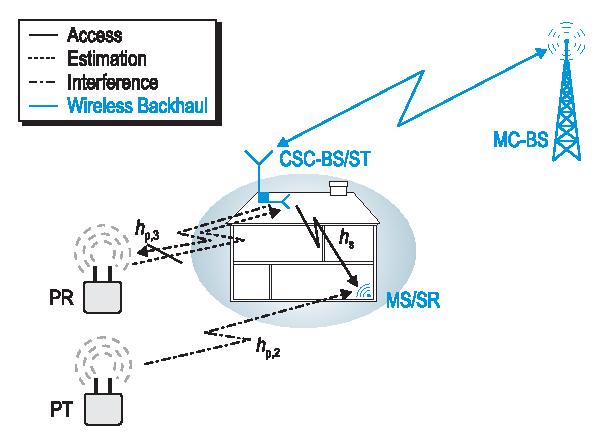
\includegraphics[width = .81 \columnwidth]{../kapitel04/figures/CR_Scenario_Underlay}	     
				};
				\only<2>
				{
					\fill[opacity = 0.2, fill = red] (1.0,1.63) rectangle (1.4,1.97);
					\fill[opacity = 0.2, fill = blue] (2.12,0.54) rectangle (2.52,.88);
					\fill[opacity = 0.2, fill = kit-green100] (2.85,1.56) rectangle (3.25,1.90);
				}
			\end{tikzpicture}
			\vspace{-10mm}	
			\begin{tikzpicture}[scale=1]
				\node[anchor=south west,inner sep=0] (image) at (0,0)
				{
					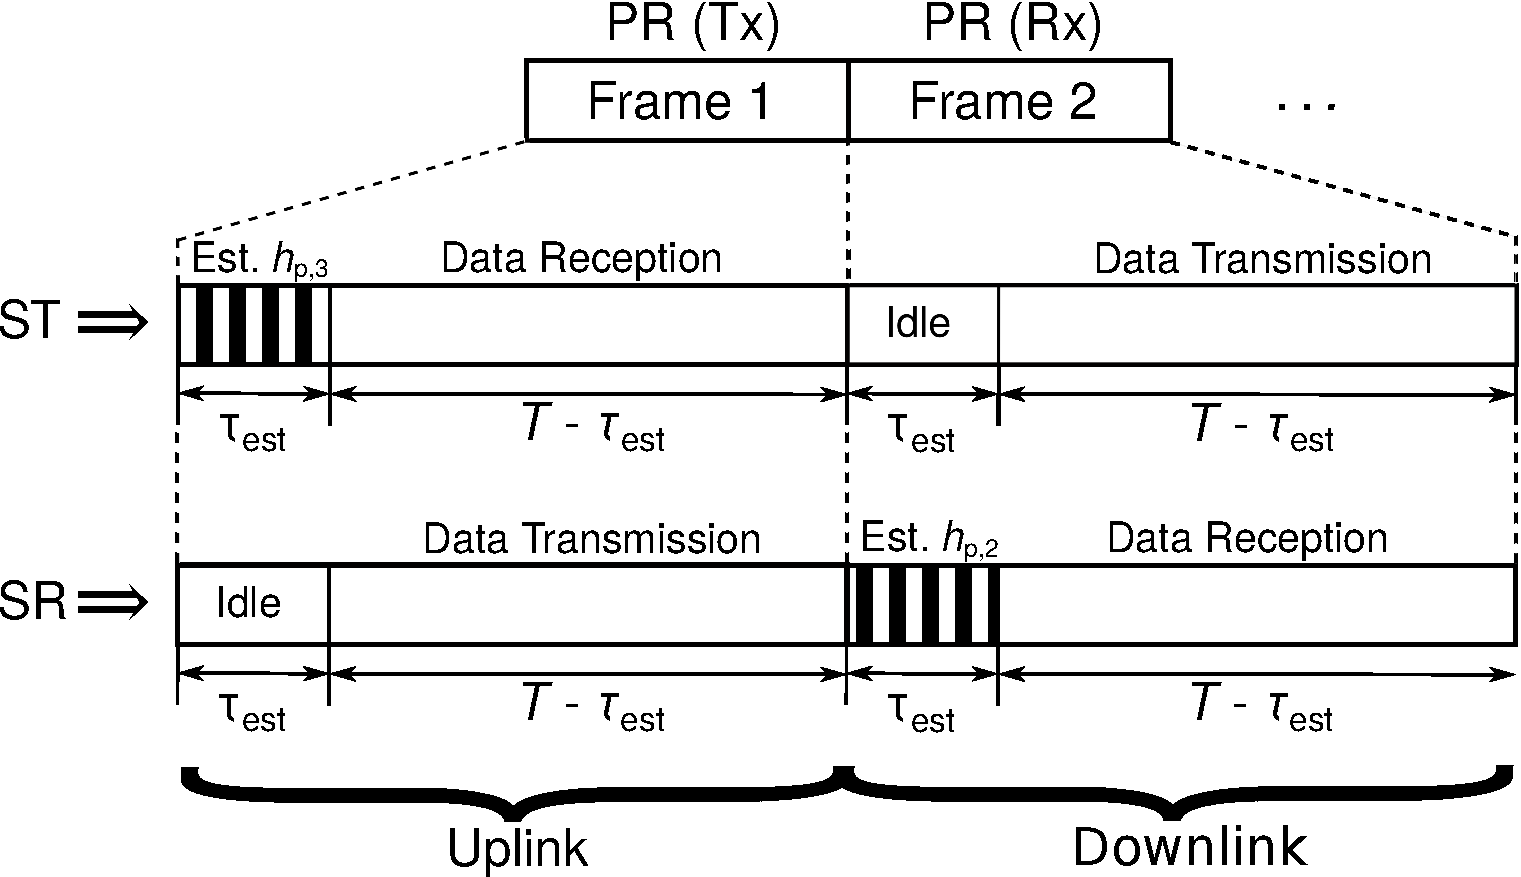
\includegraphics[width = \columnwidth]{figures/Frame_Structure_US.ps}     
				};
				\only<2->
				{
					\fill[opacity = 0.4, fill = red] (0.77,2.21) rectangle (1.41,2.54);
					\fill[opacity = 0.4, fill = blue] (3.63,1.01) rectangle (4.27,1.34);
				}
			\end{tikzpicture}	
		\end{center}
		\end{column}
	\end{columns}
\end{frame}


%%%%%%%%%%%%%%%%%%%%%%%%%%%%%%%%%%%%%%%%%%%%%%%%%%%%%%%%%%%%%%%%%%%%%%%%%%%%%%%%
\begin{frame}[t]{Underlay System}
%%%%%%%%%%%%%%%%%%%%%%%%%%%%%%%%%%%%%%%%%%%%%%%%%%%%%%%%%%%%%%%%%%%%%%%%%%%%%%%%
	\pnote{Again variations are induced due to channel estimation resulting in variations in the received power (performance parameter for the primary system) which in certain occasions can exceed the interference threshold. Such events are harmful for the operation of underlay system.} 
	\pnote{These variations are captured by means of outage constraint on the received power}
	\pnote{Besides, the transmit power is constrained, i.e., cannot be exceeded beyond a certain value}
	\pnote{Considering these two constraints the control power at ST that employs channel estimation is characterized as}
	\pnote{It is worthy to note that, in contrast to the idealistic approach, the expression of control power is influenced by channel gain via SNRp3 and the estimation time. Thus, control power allow us to capture the variations in the system.}
	\pnote{Based on this, the control power under the influence of channel estimation is classified as interference limited regime and power-limited regime (Use the expression).} 
	\pnote{At low value of test, large variations are induced in the system causing a larger of interference at the PR, hence a sever power control (low value of control power) is exercised.}
	\pnote{However, at high value of estimation time are power control is less severe, hence approaches the ideal value of the transmit power}
	\pnote{Such a phenomenon is reflected in figure, where the control increases with the estimation time for different values of the outage constraint. Obviously, stringent constraint results in a sever power control} 
	\vspace{-4.5mm}
	\fs{7}{8}
	\begin{columns}
		\begin{column}{0.45\columnwidth}
			\begin{block}{\scriptsize Control power} 
			Constraint on received interference at PR 
			\begin{align*}
				\p\left( \prcvdpr = \ephpth \preg \ge \ite \right) \le \opc, \\  
				\p\left( \left( \frac{{\color{red}{\eprcvdstpr}} - \nps}{\ptran}\right) \preg \ge \ite \right) \le \opc 
			\end{align*}
			Constraint on transmit power at ST 
			\begin{equation*}
				\preg \le \pc. \label{eq_US:pc} 
			\end{equation*}
			\end{block} 
			\vspace{-3mm}
			\begin{center}	
				\tikzfancyarrow[0.9cm][kit-green70][top color=kit-green50, bottom color=kit-green50, shape border rotate=270]{\color{kit-green50}{10}}		%	\\[0.5em]
			\end{center}	
		\end{column}
		\begin{column}{0.55\columnwidth}
		\fs{7}{8}
		\begin{center}
			%% Add psfrag entries
                	% This file is generated by the MATLAB m-file laprint.m. It can be included
% into LaTeX documents using the packages graphicx, color and psfrag.
% It is accompanied by a postscript file. A sample LaTeX file is:
%    \documentclass{article}\usepackage{graphicx,color,psfrag}
%    \begin{document}% This file is generated by the MATLAB m-file laprint.m. It can be included
% into LaTeX documents using the packages graphicx, color and psfrag.
% It is accompanied by a postscript file. A sample LaTeX file is:
%    \documentclass{article}\usepackage{graphicx,color,psfrag}
%    \begin{document}% This file is generated by the MATLAB m-file laprint.m. It can be included
% into LaTeX documents using the packages graphicx, color and psfrag.
% It is accompanied by a postscript file. A sample LaTeX file is:
%    \documentclass{article}\usepackage{graphicx,color,psfrag}
%    \begin{document}\input{fig_Preg_est_time_AWGN}\end{document}
% See http://www.mathworks.de/matlabcentral/fileexchange/loadFile.do?objectId=4638
% for recent versions of laprint.m.
%
% created by:           LaPrint version 3.16 (13.9.2004)
% created on:           15-Dec-2015 22:25:07
% eps bounding box:     16 cm x 12 cm
% comment:              
%
%\begin{psfrags}%
%\psfragscanon%
%
% text strings:
\psfrag{s05}[b][b]{\fontsize{8.5}{12.75}\fontseries{m}\mathversion{normal}\fontshape{n}\selectfont \color[rgb]{0,0,0}\setlength{\tabcolsep}{0pt}\begin{tabular}{c}$\preg$ [dBm]\end{tabular}}%
\psfrag{s06}[t][t]{\fontsize{8.5}{12.75}\fontseries{m}\mathversion{normal}\fontshape{n}\selectfont \color[rgb]{0,0,0}\setlength{\tabcolsep}{0pt}\begin{tabular}{c}$\test$ [ms]\end{tabular}}%
\psfrag{s10}[][]{\fontsize{10}{15}\fontseries{m}\mathversion{normal}\fontshape{n}\selectfont \color[rgb]{0,0,0}\setlength{\tabcolsep}{0pt}\begin{tabular}{c} \end{tabular}}%
\psfrag{s11}[][]{\fontsize{10}{15}\fontseries{m}\mathversion{normal}\fontshape{n}\selectfont \color[rgb]{0,0,0}\setlength{\tabcolsep}{0pt}\begin{tabular}{c} \end{tabular}}%
\psfrag{s12}[l][l]{\fontsize{8.5}{12.75}\fontseries{m}\mathversion{normal}\fontshape{n}\selectfont \color[rgb]{0,0,0}EM}%
\psfrag{s13}[l][l]{\fontsize{8.5}{12.75}\fontseries{m}\mathversion{normal}\fontshape{n}\selectfont \color[rgb]{0,0,0}IM}%
\psfrag{s14}[l][l]{\fontsize{8.5}{12.75}\fontseries{m}\mathversion{normal}\fontshape{n}\selectfont \color[rgb]{0,0,0}EM}%
%
% axes font properties:
\fontsize{8.5}{12.75}\fontseries{m}\mathversion{normal}%
\fontshape{n}\selectfont%
%
% xticklabels:
\psfrag{x01}[t][t]{$10^{-3}$}%
\psfrag{x02}[t][t]{$10^{-2}$}%
\psfrag{x03}[t][t]{$10^{-1}$}%
\psfrag{x04}[t][t]{$10^{0}$}%
\psfrag{x05}[t][t]{$10^{1}$}%
%
% yticklabels:
\psfrag{v01}[r][r]{-20}%
\psfrag{v02}[r][r]{-19}%
\psfrag{v03}[r][r]{-18}%
\psfrag{v04}[r][r]{-17}%
\psfrag{v05}[r][r]{-16}%
\psfrag{v06}[r][r]{-15}%
\psfrag{v07}[r][r]{-14}%
\psfrag{v08}[r][r]{-13}%
\psfrag{v09}[r][r]{-12}%
\psfrag{v10}[r][r]{-11}%
\psfrag{v11}[r][r]{-10}%
\psfrag{v12}[r][r]{-9}%
%
% Figure:
%\resizebox{8cm}{!}{\includegraphics{fig_Preg_est_time_AWGN.eps}}%
%\end{psfrags}%
%
% End fig_Preg_est_time_AWGN.tex
\end{document}
% See http://www.mathworks.de/matlabcentral/fileexchange/loadFile.do?objectId=4638
% for recent versions of laprint.m.
%
% created by:           LaPrint version 3.16 (13.9.2004)
% created on:           15-Dec-2015 22:25:07
% eps bounding box:     16 cm x 12 cm
% comment:              
%
%\begin{psfrags}%
%\psfragscanon%
%
% text strings:
\psfrag{s05}[b][b]{\fontsize{8.5}{12.75}\fontseries{m}\mathversion{normal}\fontshape{n}\selectfont \color[rgb]{0,0,0}\setlength{\tabcolsep}{0pt}\begin{tabular}{c}$\preg$ [dBm]\end{tabular}}%
\psfrag{s06}[t][t]{\fontsize{8.5}{12.75}\fontseries{m}\mathversion{normal}\fontshape{n}\selectfont \color[rgb]{0,0,0}\setlength{\tabcolsep}{0pt}\begin{tabular}{c}$\test$ [ms]\end{tabular}}%
\psfrag{s10}[][]{\fontsize{10}{15}\fontseries{m}\mathversion{normal}\fontshape{n}\selectfont \color[rgb]{0,0,0}\setlength{\tabcolsep}{0pt}\begin{tabular}{c} \end{tabular}}%
\psfrag{s11}[][]{\fontsize{10}{15}\fontseries{m}\mathversion{normal}\fontshape{n}\selectfont \color[rgb]{0,0,0}\setlength{\tabcolsep}{0pt}\begin{tabular}{c} \end{tabular}}%
\psfrag{s12}[l][l]{\fontsize{8.5}{12.75}\fontseries{m}\mathversion{normal}\fontshape{n}\selectfont \color[rgb]{0,0,0}EM}%
\psfrag{s13}[l][l]{\fontsize{8.5}{12.75}\fontseries{m}\mathversion{normal}\fontshape{n}\selectfont \color[rgb]{0,0,0}IM}%
\psfrag{s14}[l][l]{\fontsize{8.5}{12.75}\fontseries{m}\mathversion{normal}\fontshape{n}\selectfont \color[rgb]{0,0,0}EM}%
%
% axes font properties:
\fontsize{8.5}{12.75}\fontseries{m}\mathversion{normal}%
\fontshape{n}\selectfont%
%
% xticklabels:
\psfrag{x01}[t][t]{$10^{-3}$}%
\psfrag{x02}[t][t]{$10^{-2}$}%
\psfrag{x03}[t][t]{$10^{-1}$}%
\psfrag{x04}[t][t]{$10^{0}$}%
\psfrag{x05}[t][t]{$10^{1}$}%
%
% yticklabels:
\psfrag{v01}[r][r]{-20}%
\psfrag{v02}[r][r]{-19}%
\psfrag{v03}[r][r]{-18}%
\psfrag{v04}[r][r]{-17}%
\psfrag{v05}[r][r]{-16}%
\psfrag{v06}[r][r]{-15}%
\psfrag{v07}[r][r]{-14}%
\psfrag{v08}[r][r]{-13}%
\psfrag{v09}[r][r]{-12}%
\psfrag{v10}[r][r]{-11}%
\psfrag{v11}[r][r]{-10}%
\psfrag{v12}[r][r]{-9}%
%
% Figure:
%\resizebox{8cm}{!}{\includegraphics{fig_Preg_est_time_AWGN.eps}}%
%\end{psfrags}%
%
% End fig_Preg_est_time_AWGN.tex
\end{document}
% See http://www.mathworks.de/matlabcentral/fileexchange/loadFile.do?objectId=4638
% for recent versions of laprint.m.
%
% created by:           LaPrint version 3.16 (13.9.2004)
% created on:           15-Dec-2015 22:25:07
% eps bounding box:     16 cm x 12 cm
% comment:              
%
%\begin{psfrags}%
%\psfragscanon%
%
% text strings:
\psfrag{s05}[b][b]{\fontsize{8.5}{12.75}\fontseries{m}\mathversion{normal}\fontshape{n}\selectfont \color[rgb]{0,0,0}\setlength{\tabcolsep}{0pt}\begin{tabular}{c}$\preg$ [dBm]\end{tabular}}%
\psfrag{s06}[t][t]{\fontsize{8.5}{12.75}\fontseries{m}\mathversion{normal}\fontshape{n}\selectfont \color[rgb]{0,0,0}\setlength{\tabcolsep}{0pt}\begin{tabular}{c}$\test$ [ms]\end{tabular}}%
\psfrag{s10}[][]{\fontsize{10}{15}\fontseries{m}\mathversion{normal}\fontshape{n}\selectfont \color[rgb]{0,0,0}\setlength{\tabcolsep}{0pt}\begin{tabular}{c} \end{tabular}}%
\psfrag{s11}[][]{\fontsize{10}{15}\fontseries{m}\mathversion{normal}\fontshape{n}\selectfont \color[rgb]{0,0,0}\setlength{\tabcolsep}{0pt}\begin{tabular}{c} \end{tabular}}%
\psfrag{s12}[l][l]{\fontsize{8.5}{12.75}\fontseries{m}\mathversion{normal}\fontshape{n}\selectfont \color[rgb]{0,0,0}EM}%
\psfrag{s13}[l][l]{\fontsize{8.5}{12.75}\fontseries{m}\mathversion{normal}\fontshape{n}\selectfont \color[rgb]{0,0,0}IM}%
\psfrag{s14}[l][l]{\fontsize{8.5}{12.75}\fontseries{m}\mathversion{normal}\fontshape{n}\selectfont \color[rgb]{0,0,0}EM}%
%
% axes font properties:
\fontsize{8.5}{12.75}\fontseries{m}\mathversion{normal}%
\fontshape{n}\selectfont%
%
% xticklabels:
\psfrag{x01}[t][t]{$10^{-3}$}%
\psfrag{x02}[t][t]{$10^{-2}$}%
\psfrag{x03}[t][t]{$10^{-1}$}%
\psfrag{x04}[t][t]{$10^{0}$}%
\psfrag{x05}[t][t]{$10^{1}$}%
%
% yticklabels:
\psfrag{v01}[r][r]{-20}%
\psfrag{v02}[r][r]{-19}%
\psfrag{v03}[r][r]{-18}%
\psfrag{v04}[r][r]{-17}%
\psfrag{v05}[r][r]{-16}%
\psfrag{v06}[r][r]{-15}%
\psfrag{v07}[r][r]{-14}%
\psfrag{v08}[r][r]{-13}%
\psfrag{v09}[r][r]{-12}%
\psfrag{v10}[r][r]{-11}%
\psfrag{v11}[r][r]{-10}%
\psfrag{v12}[r][r]{-9}%
%
% Figure:
%\resizebox{8cm}{!}{\includegraphics{fig_Preg_est_time_AWGN.eps}}%
%\end{psfrags}%
%
% End fig_Preg_est_time_AWGN.tex

			\centering
             	        \resizebox{.95 \columnwidth}{!}{%
                        \begin{tikzpicture}[scale=1]
				\node[anchor=south west,inner sep=0] (image) at (0,0)
				{
					\includegraphics[width= \figscale]{../kapitel04/figures/fig_Preg_est_time_AWGN}
				};
				\begin{scope}[x={(image.south east)},y={(image.north west)}]

				\draw (0.35,0.56) arc(-130:130:0.007 and 0.021);
				\node[draw,fill=gray!10,font=\scriptsize] at (0.44,0.515) {$\opc = 0.01$};

				\draw (0.35,0.68) arc(-130:130:0.007 and 0.021);
				\node[draw,fill=gray!10,font=\scriptsize] at (0.275,0.758) {$\opc = 0.1$};

	               		\node[draw=none,fill=kit-green30, minimum height = 0.6cm, align = center, font = \footnotesize] at (0.5, 1.05) {Control power versus estimation time};
				%\draw[help lines,xstep=.1,ystep=.1] (0,0) grid (1,1);
				%\foreach \x in {0,1,...,9} { \node [anchor=north] at (\x/10,0) {0.\x}; }
				%\foreach \y in {0,1,...,9} { \node [anchor=east] at (0,\y/10) {0.\y}; }
				\end{scope}
			\end{tikzpicture}
                }
		\end{center}
		\end{column}
	\end{columns}
	\begin{block}{}%{\scriptsize Power control} 
		\vspace{-4mm}
		\begin{align*}
			\preg &= 
			\begin{cases} 
				\frac{\ite \ptran}{ \left(\bpo \Gamma^{-1}(\opc, \apo) - \nps  \right)}, & \mbox{for } \preg < \pc \Rightarrow \text{Interference-limited regime}\\
				\pc, & \mbox{for } \preg \ge \pc \Rightarrow \text{Power-limited regime}
				\end{cases} \\
				\text{where  } \apo &= \frac{{\color{kit-green100}{\test \fsam}} (1 + \snrrcvdu)^2}{2 + 4 \snrrcvdu} \text{ and } \bpo = \frac{\nps (2 + 4 \snrrcvdu)}{{\color{kit-green100}{\test \fsam}} (1 + \snrrcvdu)},
			\end{align*}
	\end{block}
\end{frame}


%%%%%%%%%%%%%%%%%%%%%%%%%%%%%%%%%%%%%%%%%%%%%%%%%%%%%%%%%%%%%%%%%%%%%%%%%%%%%%%%
\begin{frame}[t]{Underlay System}
%%%%%%%%%%%%%%%%%%%%%%%%%%%%%%%%%%%%%%%%%%%%%%%%%%%%%%%%%%%%%%%%%%%%%%%%%%%%%%%%
	%\vspace{-4.5mm}
	\fs{7}{8}
	\begin{columns}
		\begin{column}{0.45\columnwidth}
			\begin{block}{\scriptsize Secondary throughput} %{\scriptsize Principle}
			\vspace{-3mm}
			\begin{align*}
				\eca  = \log_2 \left(1 + \frac{{\color{kit-green100}{\epgs}} \preg}{{\color{blue}{\eprcvdsr}}} \right) \\
				\rs(\test) = \frac{T - \test}{T} \e{\eca} {\eca} 
			\end{align*}
			\end{block}

			\begin{block}{\scriptsize Achievable secondary throughput} 
			\vspace{-3mm}
			\begin{align*}
				\trs(\ttest)  = \maxi_{\test}  & \text{      } {\rs(\test)} \\
				\text{s.t.} & \;\p\left( \ephpth \preg \ge \ite \right) \le \opc \\
				\text{s.t.} & \;\preg \le \pc
			\end{align*}
			\end{block}
		\end{column}
		\begin{column}{0.55\columnwidth}
		\fs{7}{8}
		\begin{center}
			\centering
             	        \resizebox{.95 \columnwidth}{!}{%
                        \only<1>
			{
				%% Add psfrag entries
              		  	% This file is generated by the MATLAB m-file laprint.m. It can be included
% into LaTeX documents using the packages graphicx, color and psfrag.
% It is accompanied by a postscript file. A sample LaTeX file is:
%    \documentclass{article}\usepackage{graphicx,color,psfrag}
%    \begin{document}% This file is generated by the MATLAB m-file laprint.m. It can be included
% into LaTeX documents using the packages graphicx, color and psfrag.
% It is accompanied by a postscript file. A sample LaTeX file is:
%    \documentclass{article}\usepackage{graphicx,color,psfrag}
%    \begin{document}% This file is generated by the MATLAB m-file laprint.m. It can be included
% into LaTeX documents using the packages graphicx, color and psfrag.
% It is accompanied by a postscript file. A sample LaTeX file is:
%    \documentclass{article}\usepackage{graphicx,color,psfrag}
%    \begin{document}\input{fig_thr_est_time_tradeoff_AWGN}\end{document}
% See http://www.mathworks.de/matlabcentral/fileexchange/loadFile.do?objectId=4638
% for recent versions of laprint.m.
%
% created by:           LaPrint version 3.16 (13.9.2004)
% created on:           08-Jan-2016 12:22:27
% eps bounding box:     16 cm x 12 cm
% comment:              
%
%\begin{psfrags}%
%\psfragscanon%
%
% text strings:
\psfrag{s05}[b][b]{\fontsize{8.5}{12.75}\fontseries{m}\mathversion{normal}\fontshape{n}\selectfont \color[rgb]{0,0,0}\setlength{\tabcolsep}{0pt}\begin{tabular}{c}$\rs(\tau)$ [bits/sec/Hz]\end{tabular}}%
\psfrag{s06}[t][t]{\fontsize{8.5}{12.75}\fontseries{m}\mathversion{normal}\fontshape{n}\selectfont \color[rgb]{0,0,0}\setlength{\tabcolsep}{0pt}\begin{tabular}{c}$\tau$ [ms]\end{tabular}}%
\psfrag{s10}[][]{\fontsize{10}{15}\fontseries{m}\mathversion{normal}\fontshape{n}\selectfont \color[rgb]{0,0,0}\setlength{\tabcolsep}{0pt}\begin{tabular}{c} \end{tabular}}%
\psfrag{s11}[][]{\fontsize{10}{15}\fontseries{m}\mathversion{normal}\fontshape{n}\selectfont \color[rgb]{0,0,0}\setlength{\tabcolsep}{0pt}\begin{tabular}{c} \end{tabular}}%
\psfrag{s12}[l][l]{\fontsize{8.5}{12.75}\fontseries{m}\mathversion{normal}\fontshape{n}\selectfont \color[rgb]{0,0,0}Simulated}%
\psfrag{s13}[l][l]{\fontsize{8.5}{12.75}\fontseries{m}\mathversion{normal}\fontshape{n}\selectfont \color[rgb]{0,0,0}IM}%
\psfrag{s14}[l][l]{\fontsize{8.5}{12.75}\fontseries{m}\mathversion{normal}\fontshape{n}\selectfont \color[rgb]{0,0,0}EM}%
\psfrag{s15}[l][l]{\fontsize{8.5}{12.75}\fontseries{m}\mathversion{normal}\fontshape{n}\selectfont \color[rgb]{0,0,0}$\trs(\ttau)$}%
\psfrag{s16}[l][l]{\fontsize{8.5}{12.75}\fontseries{m}\mathversion{normal}\fontshape{n}\selectfont \color[rgb]{0,0,0}Simulated}%
%
% axes font properties:
\fontsize{8.5}{12.75}\fontseries{m}\mathversion{normal}%
\fontshape{n}\selectfont%
%
% xticklabels:
\psfrag{x01}[t][t]{0}%
\psfrag{x02}[t][t]{1}%
\psfrag{x03}[t][t]{2}%
\psfrag{x04}[t][t]{3}%
\psfrag{x05}[t][t]{4}%
\psfrag{x06}[t][t]{5}%
\psfrag{x07}[t][t]{6}%
\psfrag{x08}[t][t]{7}%
\psfrag{x09}[t][t]{8}%
\psfrag{x10}[t][t]{9}%
\psfrag{x11}[t][t]{10}%
%
% yticklabels:
\psfrag{v01}[r][r]{1.6}%
\psfrag{v02}[r][r]{1.8}%
\psfrag{v03}[r][r]{2}%
\psfrag{v04}[r][r]{2.2}%
\psfrag{v05}[r][r]{2.4}%
\psfrag{v06}[r][r]{2.6}%
%
% Figure:
%\resizebox{8cm}{!}{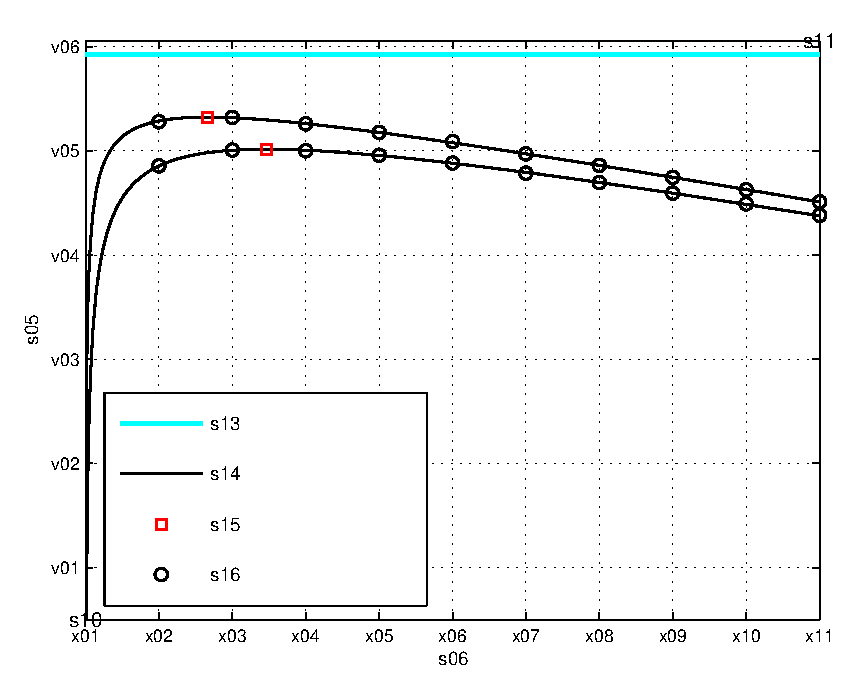
\includegraphics{fig_thr_est_time_tradeoff_AWGN.eps}}%
%\end{psfrags}%
%
% End fig_thr_est_time_tradeoff_AWGN.tex
\end{document}
% See http://www.mathworks.de/matlabcentral/fileexchange/loadFile.do?objectId=4638
% for recent versions of laprint.m.
%
% created by:           LaPrint version 3.16 (13.9.2004)
% created on:           08-Jan-2016 12:22:27
% eps bounding box:     16 cm x 12 cm
% comment:              
%
%\begin{psfrags}%
%\psfragscanon%
%
% text strings:
\psfrag{s05}[b][b]{\fontsize{8.5}{12.75}\fontseries{m}\mathversion{normal}\fontshape{n}\selectfont \color[rgb]{0,0,0}\setlength{\tabcolsep}{0pt}\begin{tabular}{c}$\rs(\tau)$ [bits/sec/Hz]\end{tabular}}%
\psfrag{s06}[t][t]{\fontsize{8.5}{12.75}\fontseries{m}\mathversion{normal}\fontshape{n}\selectfont \color[rgb]{0,0,0}\setlength{\tabcolsep}{0pt}\begin{tabular}{c}$\tau$ [ms]\end{tabular}}%
\psfrag{s10}[][]{\fontsize{10}{15}\fontseries{m}\mathversion{normal}\fontshape{n}\selectfont \color[rgb]{0,0,0}\setlength{\tabcolsep}{0pt}\begin{tabular}{c} \end{tabular}}%
\psfrag{s11}[][]{\fontsize{10}{15}\fontseries{m}\mathversion{normal}\fontshape{n}\selectfont \color[rgb]{0,0,0}\setlength{\tabcolsep}{0pt}\begin{tabular}{c} \end{tabular}}%
\psfrag{s12}[l][l]{\fontsize{8.5}{12.75}\fontseries{m}\mathversion{normal}\fontshape{n}\selectfont \color[rgb]{0,0,0}Simulated}%
\psfrag{s13}[l][l]{\fontsize{8.5}{12.75}\fontseries{m}\mathversion{normal}\fontshape{n}\selectfont \color[rgb]{0,0,0}IM}%
\psfrag{s14}[l][l]{\fontsize{8.5}{12.75}\fontseries{m}\mathversion{normal}\fontshape{n}\selectfont \color[rgb]{0,0,0}EM}%
\psfrag{s15}[l][l]{\fontsize{8.5}{12.75}\fontseries{m}\mathversion{normal}\fontshape{n}\selectfont \color[rgb]{0,0,0}$\trs(\ttau)$}%
\psfrag{s16}[l][l]{\fontsize{8.5}{12.75}\fontseries{m}\mathversion{normal}\fontshape{n}\selectfont \color[rgb]{0,0,0}Simulated}%
%
% axes font properties:
\fontsize{8.5}{12.75}\fontseries{m}\mathversion{normal}%
\fontshape{n}\selectfont%
%
% xticklabels:
\psfrag{x01}[t][t]{0}%
\psfrag{x02}[t][t]{1}%
\psfrag{x03}[t][t]{2}%
\psfrag{x04}[t][t]{3}%
\psfrag{x05}[t][t]{4}%
\psfrag{x06}[t][t]{5}%
\psfrag{x07}[t][t]{6}%
\psfrag{x08}[t][t]{7}%
\psfrag{x09}[t][t]{8}%
\psfrag{x10}[t][t]{9}%
\psfrag{x11}[t][t]{10}%
%
% yticklabels:
\psfrag{v01}[r][r]{1.6}%
\psfrag{v02}[r][r]{1.8}%
\psfrag{v03}[r][r]{2}%
\psfrag{v04}[r][r]{2.2}%
\psfrag{v05}[r][r]{2.4}%
\psfrag{v06}[r][r]{2.6}%
%
% Figure:
%\resizebox{8cm}{!}{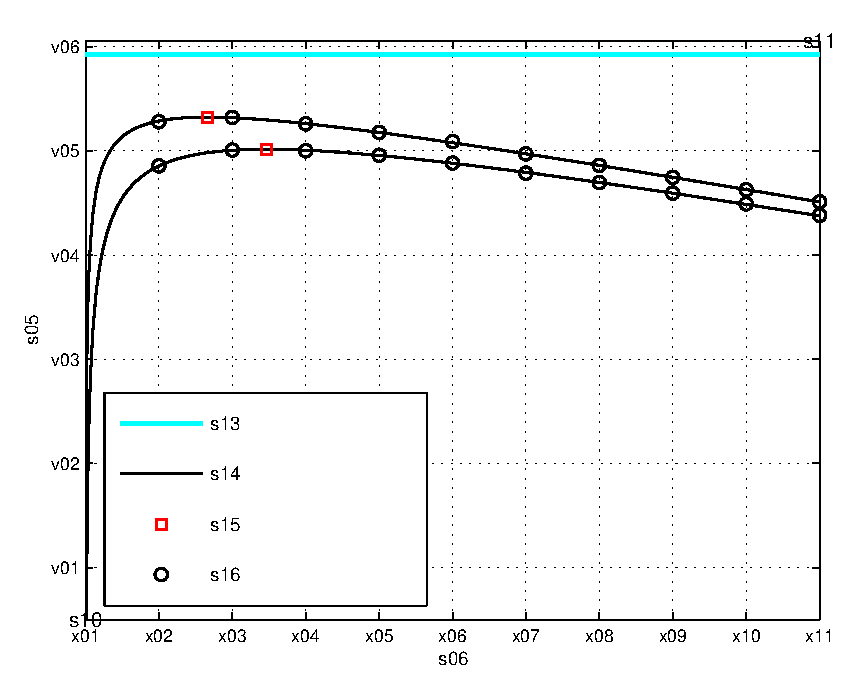
\includegraphics{fig_thr_est_time_tradeoff_AWGN.eps}}%
%\end{psfrags}%
%
% End fig_thr_est_time_tradeoff_AWGN.tex
\end{document}
% See http://www.mathworks.de/matlabcentral/fileexchange/loadFile.do?objectId=4638
% for recent versions of laprint.m.
%
% created by:           LaPrint version 3.16 (13.9.2004)
% created on:           08-Jan-2016 12:22:27
% eps bounding box:     16 cm x 12 cm
% comment:              
%
%\begin{psfrags}%
%\psfragscanon%
%
% text strings:
\psfrag{s05}[b][b]{\fontsize{8.5}{12.75}\fontseries{m}\mathversion{normal}\fontshape{n}\selectfont \color[rgb]{0,0,0}\setlength{\tabcolsep}{0pt}\begin{tabular}{c}$\rs(\tau)$ [bits/sec/Hz]\end{tabular}}%
\psfrag{s06}[t][t]{\fontsize{8.5}{12.75}\fontseries{m}\mathversion{normal}\fontshape{n}\selectfont \color[rgb]{0,0,0}\setlength{\tabcolsep}{0pt}\begin{tabular}{c}$\tau$ [ms]\end{tabular}}%
\psfrag{s10}[][]{\fontsize{10}{15}\fontseries{m}\mathversion{normal}\fontshape{n}\selectfont \color[rgb]{0,0,0}\setlength{\tabcolsep}{0pt}\begin{tabular}{c} \end{tabular}}%
\psfrag{s11}[][]{\fontsize{10}{15}\fontseries{m}\mathversion{normal}\fontshape{n}\selectfont \color[rgb]{0,0,0}\setlength{\tabcolsep}{0pt}\begin{tabular}{c} \end{tabular}}%
\psfrag{s12}[l][l]{\fontsize{8.5}{12.75}\fontseries{m}\mathversion{normal}\fontshape{n}\selectfont \color[rgb]{0,0,0}Simulated}%
\psfrag{s13}[l][l]{\fontsize{8.5}{12.75}\fontseries{m}\mathversion{normal}\fontshape{n}\selectfont \color[rgb]{0,0,0}IM}%
\psfrag{s14}[l][l]{\fontsize{8.5}{12.75}\fontseries{m}\mathversion{normal}\fontshape{n}\selectfont \color[rgb]{0,0,0}EM}%
\psfrag{s15}[l][l]{\fontsize{8.5}{12.75}\fontseries{m}\mathversion{normal}\fontshape{n}\selectfont \color[rgb]{0,0,0}$\trs(\ttau)$}%
\psfrag{s16}[l][l]{\fontsize{8.5}{12.75}\fontseries{m}\mathversion{normal}\fontshape{n}\selectfont \color[rgb]{0,0,0}Simulated}%
%
% axes font properties:
\fontsize{8.5}{12.75}\fontseries{m}\mathversion{normal}%
\fontshape{n}\selectfont%
%
% xticklabels:
\psfrag{x01}[t][t]{0}%
\psfrag{x02}[t][t]{1}%
\psfrag{x03}[t][t]{2}%
\psfrag{x04}[t][t]{3}%
\psfrag{x05}[t][t]{4}%
\psfrag{x06}[t][t]{5}%
\psfrag{x07}[t][t]{6}%
\psfrag{x08}[t][t]{7}%
\psfrag{x09}[t][t]{8}%
\psfrag{x10}[t][t]{9}%
\psfrag{x11}[t][t]{10}%
%
% yticklabels:
\psfrag{v01}[r][r]{1.6}%
\psfrag{v02}[r][r]{1.8}%
\psfrag{v03}[r][r]{2}%
\psfrag{v04}[r][r]{2.2}%
\psfrag{v05}[r][r]{2.4}%
\psfrag{v06}[r][r]{2.6}%
%
% Figure:
%\resizebox{8cm}{!}{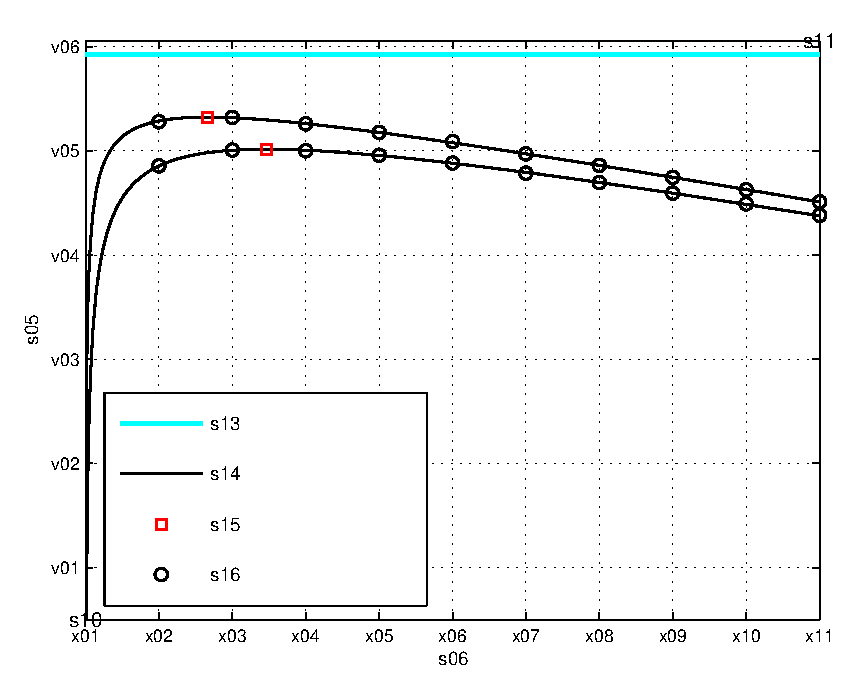
\includegraphics{fig_thr_est_time_tradeoff_AWGN.eps}}%
%\end{psfrags}%
%
% End fig_thr_est_time_tradeoff_AWGN.tex

				\begin{tikzpicture}[scale=1]
					\node[anchor=south west,inner sep=0] (image) at (0,0)
					{
					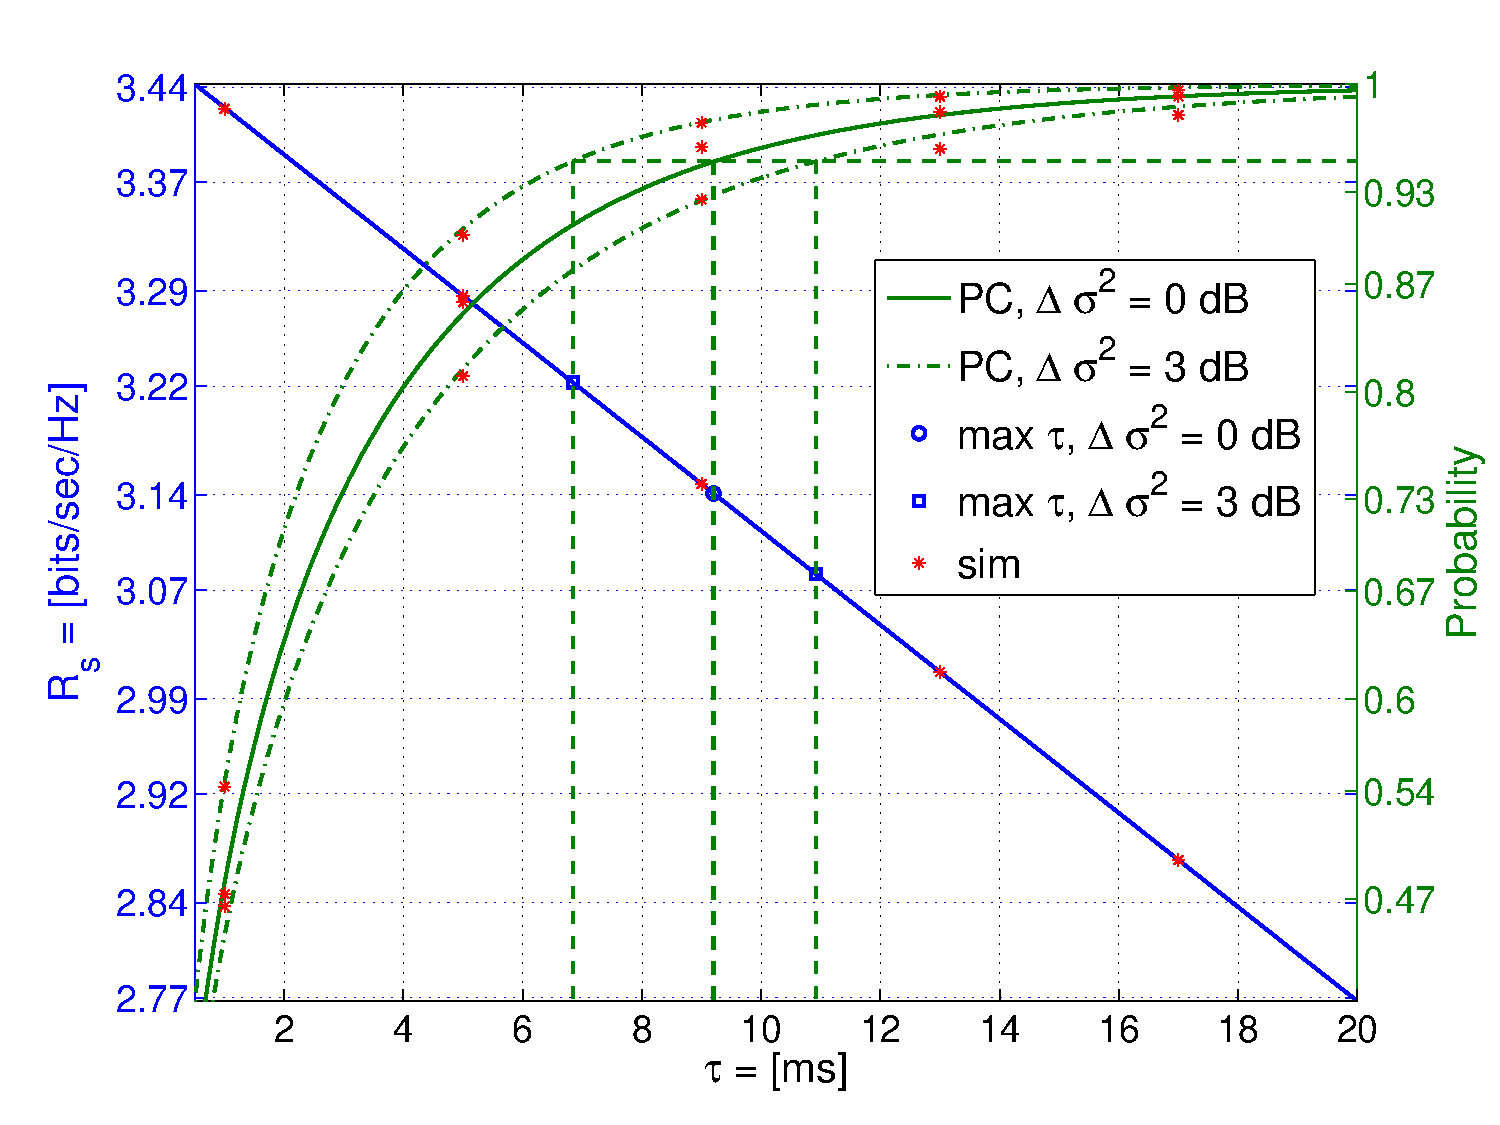
\includegraphics[width= \figscale]{../kapitel04/figures/fig_thr_est_time_tradeoff_AWGN}
};
					\begin{scope}[x={(image.south east)},y={(image.north west)}]

					\draw (0.38,0.78) arc(-130:130:0.005 and 0.015);
					\node[draw, fill=gray!10,font=\scriptsize] at (0.39,0.735) {$\opc = 0.01$};

					\draw (0.65,0.77) arc(-130:130:0.005 and 0.015);
					\node[draw,fill=gray!10,font=\scriptsize] at (0.66,0.838) {$\opc = 0.1$};
					\node[draw=none,fill=kit-green30, minimum height = 0.6cm, align = center, font = \footnotesize] at (0.5, 1.05) {Estimation-throughput tradeoff};

					%\draw[help lines,xstep=.1,ystep=.1] (0,0) grid (1,1);
					%\foreach \x in {0,1,...,9} { \node [anchor=north] at (\x/10,0) {0.\x}; }
					%\foreach \y in {0,1,...,9} { \node [anchor=east] at (0,\y/10) {0.\y}; }
				\end{scope}
				\end{tikzpicture}
			}
                        \only<2>
			{
				% This file is generated by the MATLAB m-file laprint.m. It can be included
% into LaTeX documents using the packages graphicx, color and psfrag.
% It is accompanied by a postscript file. A sample LaTeX file is:
%    \documentclass{article}\usepackage{graphicx,color,psfrag}
%    \begin{document}% This file is generated by the MATLAB m-file laprint.m. It can be included
% into LaTeX documents using the packages graphicx, color and psfrag.
% It is accompanied by a postscript file. A sample LaTeX file is:
%    \documentclass{article}\usepackage{graphicx,color,psfrag}
%    \begin{document}% This file is generated by the MATLAB m-file laprint.m. It can be included
% into LaTeX documents using the packages graphicx, color and psfrag.
% It is accompanied by a postscript file. A sample LaTeX file is:
%    \documentclass{article}\usepackage{graphicx,color,psfrag}
%    \begin{document}\input{fig_opt_thr_vs_SNR_AWGN_SI_00}\end{document}
% See http://www.mathworks.de/matlabcentral/fileexchange/loadFile.do?objectId=4638
% for recent versions of laprint.m.
%
% created by:           LaPrint version 3.16 (13.9.2004)
% created on:           08-Jan-2016 18:59:26
% eps bounding box:     16 cm x 12 cm
% comment:              
%
%\begin{psfrags}%
%\psfragscanon%
%
% text strings:
\psfrag{s05}[b][b]{\fontsize{8.5}{12.75}\fontseries{m}\mathversion{normal}\fontshape{n}\selectfont \color[rgb]{0,0,0}\setlength{\tabcolsep}{0pt}\begin{tabular}{c}$\rs(\ttest)$ [bits/sec/Hz]\end{tabular}}%
\psfrag{s06}[t][t]{\fontsize{8.5}{12.75}\fontseries{m}\mathversion{normal}\fontshape{n}\selectfont \color[rgb]{0,0,0}\setlength{\tabcolsep}{0pt}\begin{tabular}{c}$\snrrcvdu$ [dB]\end{tabular}}%
\psfrag{s10}[][]{\fontsize{10}{15}\fontseries{m}\mathversion{normal}\fontshape{n}\selectfont \color[rgb]{0,0,0}\setlength{\tabcolsep}{0pt}\begin{tabular}{c} \end{tabular}}%
\psfrag{s11}[][]{\fontsize{10}{15}\fontseries{m}\mathversion{normal}\fontshape{n}\selectfont \color[rgb]{0,0,0}\setlength{\tabcolsep}{0pt}\begin{tabular}{c} \end{tabular}}%
\psfrag{s12}[l][l]{\fontsize{8.5}{12.75}\fontseries{m}\mathversion{normal}\fontshape{n}\selectfont \color[rgb]{0,0,0}Coro 3}%
\psfrag{s13}[l][l]{\fontsize{8.5}{12.75}\fontseries{m}\mathversion{normal}\fontshape{n}\selectfont \color[rgb]{0,0,0}IM}%
\psfrag{s14}[l][l]{\fontsize{8.5}{12.75}\fontseries{m}\mathversion{normal}\fontshape{n}\selectfont \color[rgb]{0,0,0}EM}%
\psfrag{s15}[l][l]{\fontsize{8.5}{12.75}\fontseries{m}\mathversion{normal}\fontshape{n}\selectfont \color[rgb]{0,0,0}Coro 3}%
%
% axes font properties:
\fontsize{8.5}{12.75}\fontseries{m}\mathversion{normal}%
\fontshape{n}\selectfont%
%
% xticklabels:
\psfrag{x01}[t][t]{-20}%
\psfrag{x02}[t][t]{-15}%
\psfrag{x03}[t][t]{-10}%
\psfrag{x04}[t][t]{-5}%
\psfrag{x05}[t][t]{0}%
\psfrag{x06}[t][t]{5}%
\psfrag{x07}[t][t]{10}%
%
% yticklabels:
\psfrag{v01}[r][r]{0}%
\psfrag{v02}[r][r]{1}%
\psfrag{v03}[r][r]{2}%
\psfrag{v04}[r][r]{3}%
\psfrag{v05}[r][r]{4}%
\psfrag{v06}[r][r]{5}%
\psfrag{v07}[r][r]{6}%
\psfrag{v08}[r][r]{7}%
\psfrag{v09}[r][r]{8}%
\psfrag{v10}[r][r]{9}%
%
% Figure:
%\resizebox{8cm}{!}{\includegraphics{fig_opt_thr_vs_SNR_AWGN_SI_00.eps}}%
%\end{psfrags}%
%
% End fig_opt_thr_vs_SNR_AWGN_SI_00.tex
\end{document}
% See http://www.mathworks.de/matlabcentral/fileexchange/loadFile.do?objectId=4638
% for recent versions of laprint.m.
%
% created by:           LaPrint version 3.16 (13.9.2004)
% created on:           08-Jan-2016 18:59:26
% eps bounding box:     16 cm x 12 cm
% comment:              
%
%\begin{psfrags}%
%\psfragscanon%
%
% text strings:
\psfrag{s05}[b][b]{\fontsize{8.5}{12.75}\fontseries{m}\mathversion{normal}\fontshape{n}\selectfont \color[rgb]{0,0,0}\setlength{\tabcolsep}{0pt}\begin{tabular}{c}$\rs(\ttest)$ [bits/sec/Hz]\end{tabular}}%
\psfrag{s06}[t][t]{\fontsize{8.5}{12.75}\fontseries{m}\mathversion{normal}\fontshape{n}\selectfont \color[rgb]{0,0,0}\setlength{\tabcolsep}{0pt}\begin{tabular}{c}$\snrrcvdu$ [dB]\end{tabular}}%
\psfrag{s10}[][]{\fontsize{10}{15}\fontseries{m}\mathversion{normal}\fontshape{n}\selectfont \color[rgb]{0,0,0}\setlength{\tabcolsep}{0pt}\begin{tabular}{c} \end{tabular}}%
\psfrag{s11}[][]{\fontsize{10}{15}\fontseries{m}\mathversion{normal}\fontshape{n}\selectfont \color[rgb]{0,0,0}\setlength{\tabcolsep}{0pt}\begin{tabular}{c} \end{tabular}}%
\psfrag{s12}[l][l]{\fontsize{8.5}{12.75}\fontseries{m}\mathversion{normal}\fontshape{n}\selectfont \color[rgb]{0,0,0}Coro 3}%
\psfrag{s13}[l][l]{\fontsize{8.5}{12.75}\fontseries{m}\mathversion{normal}\fontshape{n}\selectfont \color[rgb]{0,0,0}IM}%
\psfrag{s14}[l][l]{\fontsize{8.5}{12.75}\fontseries{m}\mathversion{normal}\fontshape{n}\selectfont \color[rgb]{0,0,0}EM}%
\psfrag{s15}[l][l]{\fontsize{8.5}{12.75}\fontseries{m}\mathversion{normal}\fontshape{n}\selectfont \color[rgb]{0,0,0}Coro 3}%
%
% axes font properties:
\fontsize{8.5}{12.75}\fontseries{m}\mathversion{normal}%
\fontshape{n}\selectfont%
%
% xticklabels:
\psfrag{x01}[t][t]{-20}%
\psfrag{x02}[t][t]{-15}%
\psfrag{x03}[t][t]{-10}%
\psfrag{x04}[t][t]{-5}%
\psfrag{x05}[t][t]{0}%
\psfrag{x06}[t][t]{5}%
\psfrag{x07}[t][t]{10}%
%
% yticklabels:
\psfrag{v01}[r][r]{0}%
\psfrag{v02}[r][r]{1}%
\psfrag{v03}[r][r]{2}%
\psfrag{v04}[r][r]{3}%
\psfrag{v05}[r][r]{4}%
\psfrag{v06}[r][r]{5}%
\psfrag{v07}[r][r]{6}%
\psfrag{v08}[r][r]{7}%
\psfrag{v09}[r][r]{8}%
\psfrag{v10}[r][r]{9}%
%
% Figure:
%\resizebox{8cm}{!}{\includegraphics{fig_opt_thr_vs_SNR_AWGN_SI_00.eps}}%
%\end{psfrags}%
%
% End fig_opt_thr_vs_SNR_AWGN_SI_00.tex
\end{document}
% See http://www.mathworks.de/matlabcentral/fileexchange/loadFile.do?objectId=4638
% for recent versions of laprint.m.
%
% created by:           LaPrint version 3.16 (13.9.2004)
% created on:           08-Jan-2016 18:59:26
% eps bounding box:     16 cm x 12 cm
% comment:              
%
%\begin{psfrags}%
%\psfragscanon%
%
% text strings:
\psfrag{s05}[b][b]{\fontsize{8.5}{12.75}\fontseries{m}\mathversion{normal}\fontshape{n}\selectfont \color[rgb]{0,0,0}\setlength{\tabcolsep}{0pt}\begin{tabular}{c}$\rs(\ttest)$ [bits/sec/Hz]\end{tabular}}%
\psfrag{s06}[t][t]{\fontsize{8.5}{12.75}\fontseries{m}\mathversion{normal}\fontshape{n}\selectfont \color[rgb]{0,0,0}\setlength{\tabcolsep}{0pt}\begin{tabular}{c}$\snrrcvdu$ [dB]\end{tabular}}%
\psfrag{s10}[][]{\fontsize{10}{15}\fontseries{m}\mathversion{normal}\fontshape{n}\selectfont \color[rgb]{0,0,0}\setlength{\tabcolsep}{0pt}\begin{tabular}{c} \end{tabular}}%
\psfrag{s11}[][]{\fontsize{10}{15}\fontseries{m}\mathversion{normal}\fontshape{n}\selectfont \color[rgb]{0,0,0}\setlength{\tabcolsep}{0pt}\begin{tabular}{c} \end{tabular}}%
\psfrag{s12}[l][l]{\fontsize{8.5}{12.75}\fontseries{m}\mathversion{normal}\fontshape{n}\selectfont \color[rgb]{0,0,0}Coro 3}%
\psfrag{s13}[l][l]{\fontsize{8.5}{12.75}\fontseries{m}\mathversion{normal}\fontshape{n}\selectfont \color[rgb]{0,0,0}IM}%
\psfrag{s14}[l][l]{\fontsize{8.5}{12.75}\fontseries{m}\mathversion{normal}\fontshape{n}\selectfont \color[rgb]{0,0,0}EM}%
\psfrag{s15}[l][l]{\fontsize{8.5}{12.75}\fontseries{m}\mathversion{normal}\fontshape{n}\selectfont \color[rgb]{0,0,0}Coro 3}%
%
% axes font properties:
\fontsize{8.5}{12.75}\fontseries{m}\mathversion{normal}%
\fontshape{n}\selectfont%
%
% xticklabels:
\psfrag{x01}[t][t]{-20}%
\psfrag{x02}[t][t]{-15}%
\psfrag{x03}[t][t]{-10}%
\psfrag{x04}[t][t]{-5}%
\psfrag{x05}[t][t]{0}%
\psfrag{x06}[t][t]{5}%
\psfrag{x07}[t][t]{10}%
%
% yticklabels:
\psfrag{v01}[r][r]{0}%
\psfrag{v02}[r][r]{1}%
\psfrag{v03}[r][r]{2}%
\psfrag{v04}[r][r]{3}%
\psfrag{v05}[r][r]{4}%
\psfrag{v06}[r][r]{5}%
\psfrag{v07}[r][r]{6}%
\psfrag{v08}[r][r]{7}%
\psfrag{v09}[r][r]{8}%
\psfrag{v10}[r][r]{9}%
%
% Figure:
%\resizebox{8cm}{!}{\includegraphics{fig_opt_thr_vs_SNR_AWGN_SI_00.eps}}%
%\end{psfrags}%
%
% End fig_opt_thr_vs_SNR_AWGN_SI_00.tex

				\begin{tikzpicture}[scale=1]
				\node[anchor=south west,inner sep=0] (image) at (0,0)
				{
     					\includegraphics[width= \figscale]{../kapitel04/figures/fig_opt_thr_vs_SNR_AWGN_SI_00}
				};
				\begin{scope}[x={(image.south east)},y={(image.north west)}]

				\draw (0.225,0.615) arc(-160:160:0.01 and 0.03);
				\node[draw, fill=gray!10, font=\scriptsize] (text1) at (0.7,0.725) {$\pc = \SI{00}{dBm}$};
				\draw (0.275,0.33) arc(-160:160:0.01 and 0.03);
				\node[draw, fill=gray!10, font=\scriptsize] (text2) at (0.75,0.44) {$\pc = \SI{-10}{dBm}$};
				%\draw (0.63,0.66) arc(-150:150:0.016 and 0.048);
				\draw[black, ->] (text1.west) -- (0.245,0.635);
				%\draw (0.63,0.59) arc(-160:160:0.01 and 0.03);
				\draw[black, ->] (text2.west) -- (0.295,0.35);


				\draw (0.27,0.225) arc(-160:160:0.01 and 0.03);
				\draw[black,thick,<->] (0.084,0.25) --  node[above, font=\scriptsize] {Power-limited} (0.367,0.25);
				\draw[black,thick,<->] (0.084,0.22) --  (0.667,0.22);

				\draw (0.7,0.105) arc(-160:160:0.01 and 0.03);
				\draw[black,thick,<->] (0.37,0.13) --  node[above, font=\scriptsize] {Interference-limited} (0.965,0.13);
				\draw[black,thick,<->] (0.67,0.10) --  (0.965,0.10);
					
				\node[draw=none,fill=kit-green30, minimum height = 0.6cm, align = center, font = \footnotesize] at (0.5, 1.05) {Achievable throughput versus SNR at ST over $\phpth$};

				%\draw[help lines,xstep=.1,ystep=.1] (0,0) grid (1,1);
				%\foreach \x in {0,1,...,9} { \node [anchor=north] at (\x/10,0) {0.\x}; }
				%\foreach \y in {0,1,...,9} { \node [anchor=east] at (0,\y/10) {0.\y}; }
				\end{scope}
				\end{tikzpicture}	
			}
                }
		\end{center}
		\end{column}
	\end{columns}
	\onslide<2->
	{	
		\begin{block}{}%{\scriptsize Power control} 
		\begin{itemize}
			\item Low $\snrrcvdu$ represents a weak link quality, is beneficial to secondary system 
			% Due to tansmit power constraint the operation of the US is resctricted for low of SNR
			
			\item Operation of underlay system is classified is different regimes: (i) power-limited regime and (ii) interference-limited regime
			\item The performance (operation range) of US is highly dependent on $\pfull$ 
		\end{itemize}		
		\end{block}
	}
\end{frame}
\fi

\ifhybrid
\section{Hybrid System}
%%%%%%%%%%%%%%%%%%%%%%%%%%%%%%%%%%%%%%%%%%%%%%%%%%%%%%%%%%%%%%%%%%%%%%%%%%%%%%%%
\begin{frame}[c]{}
%%%%%%%%%%%%%%%%%%%%%%%%%%%%%%%%%%%%%%%%%%%%%%%%%%%%%%%%%%%%%%%%%%%%%%%%%%%%%%%%
\begin{center}
Hybrid System
\end{center}
\end{frame}


%%%%%%%%%%%%%%%%%%%%%%%%%%%%%%%%%%%%%%%%%%%%%%%%%%%%%%%%%%%%%%%%%%%%%%%%%%%%%%%%
\begin{frame}[t]{Hybrid System}
%%%%%%%%%%%%%%%%%%%%%%%%%%%%%%%%%%%%%%%%%%%%%%%%%%%%%%%%%%%%%%%%%%%%%%%%%%%%%%%%
	\vspace{-4mm}
	\fs{7}{8}
	\begin{columns}
		\begin{column}{0.45\columnwidth}
				%\vspace{-1mm}
			\begin{block}{\scriptsize Principle} 
				\begin{itemize}
					\item Hybrid system combines the benefits of interweave and underlay systems to enhance spectral efficiency of cognitive radio systems  
					\item Spectrum sensing followed by power control is employed at ST 
				\end{itemize}
			\end{block}
			\vspace{3mm}
			\onslide<1->
			{
				%\vspace{-2mm}
				\begin{block}{\scriptsize Signal model} %{\scriptsize Signal model}
				\begin{equation*}
					\yrcvd[n] = 
					\begin{cases}
						\hpo \cdot \xp[n] + \wst[n] & : \mathcal{H}_1 \\
						\wst[n] & :\mathcal{H}_0
					\end{cases}
				\end{equation*}
				\begin{equation*}
					\ys[n] = 
					\begin{cases}
						\hs \cdot \xsfull[n] + \hptw \cdot \xp[n] + \wsr[n] \\%&: 1 - \pd \\
						\hs \cdot \xsfull[n] + \wsr[n] \\%&: 1 - \pfa \\
						\hs \cdot \xscont[n] + \hptw \cdot \xp[n] + \wsr[n] \\%&: \pd \\
						\hs \cdot \xscont[n] + \wsr[n] %&: \pfa 
					\end{cases}
				\end{equation*}
				\begin{equation*}
					\yp[n] = 
					\begin{cases}
						\hpth \cdot \xscont[n] + \wpr[n] \\% : \pd \\
						\hpth \cdot \xsfull[n] + \wpr[n] %& : 1- \pd 
					\end{cases}
				\end{equation*}
				\end{block}
			}
		\end{column}
		\begin{column}{0.55\columnwidth}
		\vspace{-12mm}
		\fs{7}{8}
		\begin{center}
			% Interacting entities
			%Interweave Scenario \\\vspace{0.2cm} 
        		\begin{tikzpicture}[scale=1]
				\node[anchor=south west,inner sep=0] (image) at (0,0)
				{
					\includegraphics[width = .72 \columnwidth]{../kapitel05/figures/CR_Scenario_Hybrid}	     
				};
				\only<1>
				{
					%\fill[opacity = 0.2, fill = blue] (.32,1.16) rectangle (1.22,1.8);
					%\fill[opacity = 0.2, fill = blue] (.32,-0.06) rectangle (1.22,0.58);
					%\fill[opacity = 0.2, fill = red] (3.65,1.18) rectangle (4.65,1.6);
					%\fill[opacity = 0.2, fill = red] (2.42,2.3) rectangle (3.88,3.08);
				}
			\end{tikzpicture}
			\vspace{-16mm}	
			\begin{tikzpicture}[scale=1]
				\node[anchor=south west,inner sep=0] (image) at (0,0)
				{
					\includegraphics[width = 1.02\columnwidth]{figures/Frame_Structure_HS.ps}     
				};
			\end{tikzpicture}	
		\end{center}
		\end{column}
	\end{columns}
\end{frame}


%%%%%%%%%%%%%%%%%%%%%%%%%%%%%%%%%%%%%%%%%%%%%%%%%%%%%%%%%%%%%%%%%%%%%%%%%%%%%%%%
\begin{frame}[t]{Hybrid System}
%%%%%%%%%%%%%%%%%%%%%%%%%%%%%%%%%%%%%%%%%%%%%%%%%%%%%%%%%%%%%%%%%%%%%%%%%%%%%%%%
	\vspace{-4.5mm}
	\fs{7}{8}
	\begin{columns}
		\begin{column}{0.45\columnwidth}
			\begin{block}{\scriptsize Secondary throughput}
				\vspace{-4.0mm}
				\begin{align*}
				\e{\epd, \ecz, \eco, \ectw, \ecth}{\rs(\tsen)} =  \frac{T - \testpr - \tsen}{T} \\ \Bigg[ (1 - \pfa) \cdot \phz \cdot \e{\ecz}{\ecz} +  \\ 
				(1 - \e{\epd}\epd) \cdot \pho \cdot \e{\eco}{\eco} +  \\ \pfa \cdot \phz \cdot \e{\ectw}{\ectw} + \nonumber  \\ 
				\e{\epd}{\epd} \cdot \pho \cdot \e{\ecth}{\ecth} \Bigg] 
				\end{align*}
			\end{block}
			\vspace{-0.5mm}
			\begin{block}{\scriptsize Interference Constraints} %{\scriptsize Principle}
			Constraint on detection probability
			\begin{align*}
				\p(\epd \le \pdd) \le \opdc 
			\end{align*}
			Constraint on received interference at PR 
			\begin{equation*}
				\p(\eprcvdpr \ge \ite) \le \opc 	
			\end{equation*}
			\end{block} 
		\end{column}
		\begin{column}{0.55\columnwidth}
		\fs{7}{8}
		\begin{center}
             	        \resizebox{.95 \columnwidth}{!}{%
                        \only<1>
			{
				\begin{tikzpicture}[scale=1]
				%	%% Add psfrag entries
					% This file is generated by the MATLAB m-file laprint.m. It can be included
% into LaTeX documents using the packages graphicx, color and psfrag.
% It is accompanied by a postscript file. A sample LaTeX file is:
%    \documentclass{article}\usepackage{graphicx,color,psfrag}
%    \begin{document}% This file is generated by the MATLAB m-file laprint.m. It can be included
% into LaTeX documents using the packages graphicx, color and psfrag.
% It is accompanied by a postscript file. A sample LaTeX file is:
%    \documentclass{article}\usepackage{graphicx,color,psfrag}
%    \begin{document}% This file is generated by the MATLAB m-file laprint.m. It can be included
% into LaTeX documents using the packages graphicx, color and psfrag.
% It is accompanied by a postscript file. A sample LaTeX file is:
%    \documentclass{article}\usepackage{graphicx,color,psfrag}
%    \begin{document}\input{fig_opt_cont_power_vs_SNR_AWGN}\end{document}
% See http://www.mathworks.de/matlabcentral/fileexchange/loadFile.do?objectId=4638
% for recent versions of laprint.m.
%
% created by:           LaPrint version 3.16 (13.9.2004)
% created on:           21-Feb-2016 20:15:44
% eps bounding box:     12 cm x 9 cm
% comment:              
%
%\begin{psfrags}%
%\psfragscanon%
%
% text strings:
\psfrag{s05}[b][b]{\fontsize{8}{12}\fontseries{m}\mathversion{normal}\fontshape{n}\selectfont \color[rgb]{0,0,0}\setlength{\tabcolsep}{0pt}\begin{tabular}{c}$\preg$ [dBm]\end{tabular}}%
\psfrag{s06}[t][t]{\fontsize{8}{12}\fontseries{m}\mathversion{normal}\fontshape{n}\selectfont \color[rgb]{0,0,0}\setlength{\tabcolsep}{0pt}\begin{tabular}{c}$\phpth$ [dB]\end{tabular}}%
\psfrag{s10}[][]{\fontsize{10}{15}\fontseries{m}\mathversion{normal}\fontshape{n}\selectfont \color[rgb]{0,0,0}\setlength{\tabcolsep}{0pt}\begin{tabular}{c} \end{tabular}}%
\psfrag{s11}[][]{\fontsize{10}{15}\fontseries{m}\mathversion{normal}\fontshape{n}\selectfont \color[rgb]{0,0,0}\setlength{\tabcolsep}{0pt}\begin{tabular}{c} \end{tabular}}%
\psfrag{s12}[l][l]{\fontsize{8}{12}\fontseries{m}\mathversion{normal}\fontshape{n}\selectfont \color[rgb]{0,0,0}EM}%
\psfrag{s13}[l][l]{\fontsize{8}{12}\fontseries{m}\mathversion{normal}\fontshape{n}\selectfont \color[rgb]{0,0,0}IM}%
\psfrag{s14}[l][l]{\fontsize{8}{12}\fontseries{m}\mathversion{normal}\fontshape{n}\selectfont \color[rgb]{0,0,0}EM}%
%
% axes font properties:
\fontsize{8}{12}\fontseries{m}\mathversion{normal}%
\fontshape{n}\selectfont%
%
% xticklabels:
\psfrag{x01}[t][t]{-110}%
\psfrag{x02}[t][t]{-105}%
\psfrag{x03}[t][t]{-100}%
\psfrag{x04}[t][t]{-95}%
\psfrag{x05}[t][t]{-90}%
%
% yticklabels:
\psfrag{v01}[r][r]{-20}%
\psfrag{v02}[r][r]{-15}%
\psfrag{v03}[r][r]{-10}%
\psfrag{v04}[r][r]{-5}%
\psfrag{v05}[r][r]{0}%
%
% Figure:
%\resizebox{6cm}{!}{\includegraphics{fig_opt_cont_power_vs_SNR_AWGN.eps}}%
%\end{psfrags}%
%
% End fig_opt_cont_power_vs_SNR_AWGN.tex
\end{document}
% See http://www.mathworks.de/matlabcentral/fileexchange/loadFile.do?objectId=4638
% for recent versions of laprint.m.
%
% created by:           LaPrint version 3.16 (13.9.2004)
% created on:           21-Feb-2016 20:15:44
% eps bounding box:     12 cm x 9 cm
% comment:              
%
%\begin{psfrags}%
%\psfragscanon%
%
% text strings:
\psfrag{s05}[b][b]{\fontsize{8}{12}\fontseries{m}\mathversion{normal}\fontshape{n}\selectfont \color[rgb]{0,0,0}\setlength{\tabcolsep}{0pt}\begin{tabular}{c}$\preg$ [dBm]\end{tabular}}%
\psfrag{s06}[t][t]{\fontsize{8}{12}\fontseries{m}\mathversion{normal}\fontshape{n}\selectfont \color[rgb]{0,0,0}\setlength{\tabcolsep}{0pt}\begin{tabular}{c}$\phpth$ [dB]\end{tabular}}%
\psfrag{s10}[][]{\fontsize{10}{15}\fontseries{m}\mathversion{normal}\fontshape{n}\selectfont \color[rgb]{0,0,0}\setlength{\tabcolsep}{0pt}\begin{tabular}{c} \end{tabular}}%
\psfrag{s11}[][]{\fontsize{10}{15}\fontseries{m}\mathversion{normal}\fontshape{n}\selectfont \color[rgb]{0,0,0}\setlength{\tabcolsep}{0pt}\begin{tabular}{c} \end{tabular}}%
\psfrag{s12}[l][l]{\fontsize{8}{12}\fontseries{m}\mathversion{normal}\fontshape{n}\selectfont \color[rgb]{0,0,0}EM}%
\psfrag{s13}[l][l]{\fontsize{8}{12}\fontseries{m}\mathversion{normal}\fontshape{n}\selectfont \color[rgb]{0,0,0}IM}%
\psfrag{s14}[l][l]{\fontsize{8}{12}\fontseries{m}\mathversion{normal}\fontshape{n}\selectfont \color[rgb]{0,0,0}EM}%
%
% axes font properties:
\fontsize{8}{12}\fontseries{m}\mathversion{normal}%
\fontshape{n}\selectfont%
%
% xticklabels:
\psfrag{x01}[t][t]{-110}%
\psfrag{x02}[t][t]{-105}%
\psfrag{x03}[t][t]{-100}%
\psfrag{x04}[t][t]{-95}%
\psfrag{x05}[t][t]{-90}%
%
% yticklabels:
\psfrag{v01}[r][r]{-20}%
\psfrag{v02}[r][r]{-15}%
\psfrag{v03}[r][r]{-10}%
\psfrag{v04}[r][r]{-5}%
\psfrag{v05}[r][r]{0}%
%
% Figure:
%\resizebox{6cm}{!}{\includegraphics{fig_opt_cont_power_vs_SNR_AWGN.eps}}%
%\end{psfrags}%
%
% End fig_opt_cont_power_vs_SNR_AWGN.tex
\end{document}
% See http://www.mathworks.de/matlabcentral/fileexchange/loadFile.do?objectId=4638
% for recent versions of laprint.m.
%
% created by:           LaPrint version 3.16 (13.9.2004)
% created on:           21-Feb-2016 20:15:44
% eps bounding box:     12 cm x 9 cm
% comment:              
%
%\begin{psfrags}%
%\psfragscanon%
%
% text strings:
\psfrag{s05}[b][b]{\fontsize{8}{12}\fontseries{m}\mathversion{normal}\fontshape{n}\selectfont \color[rgb]{0,0,0}\setlength{\tabcolsep}{0pt}\begin{tabular}{c}$\preg$ [dBm]\end{tabular}}%
\psfrag{s06}[t][t]{\fontsize{8}{12}\fontseries{m}\mathversion{normal}\fontshape{n}\selectfont \color[rgb]{0,0,0}\setlength{\tabcolsep}{0pt}\begin{tabular}{c}$\phpth$ [dB]\end{tabular}}%
\psfrag{s10}[][]{\fontsize{10}{15}\fontseries{m}\mathversion{normal}\fontshape{n}\selectfont \color[rgb]{0,0,0}\setlength{\tabcolsep}{0pt}\begin{tabular}{c} \end{tabular}}%
\psfrag{s11}[][]{\fontsize{10}{15}\fontseries{m}\mathversion{normal}\fontshape{n}\selectfont \color[rgb]{0,0,0}\setlength{\tabcolsep}{0pt}\begin{tabular}{c} \end{tabular}}%
\psfrag{s12}[l][l]{\fontsize{8}{12}\fontseries{m}\mathversion{normal}\fontshape{n}\selectfont \color[rgb]{0,0,0}EM}%
\psfrag{s13}[l][l]{\fontsize{8}{12}\fontseries{m}\mathversion{normal}\fontshape{n}\selectfont \color[rgb]{0,0,0}IM}%
\psfrag{s14}[l][l]{\fontsize{8}{12}\fontseries{m}\mathversion{normal}\fontshape{n}\selectfont \color[rgb]{0,0,0}EM}%
%
% axes font properties:
\fontsize{8}{12}\fontseries{m}\mathversion{normal}%
\fontshape{n}\selectfont%
%
% xticklabels:
\psfrag{x01}[t][t]{-110}%
\psfrag{x02}[t][t]{-105}%
\psfrag{x03}[t][t]{-100}%
\psfrag{x04}[t][t]{-95}%
\psfrag{x05}[t][t]{-90}%
%
% yticklabels:
\psfrag{v01}[r][r]{-20}%
\psfrag{v02}[r][r]{-15}%
\psfrag{v03}[r][r]{-10}%
\psfrag{v04}[r][r]{-5}%
\psfrag{v05}[r][r]{0}%
%
% Figure:
%\resizebox{6cm}{!}{\includegraphics{fig_opt_cont_power_vs_SNR_AWGN.eps}}%
%\end{psfrags}%
%
% End fig_opt_cont_power_vs_SNR_AWGN.tex

					\node[anchor=south west,inner sep=0] (image) at (0,0)
					{
						\includegraphics[width= \figscale]{../kapitel05/figures/fig_opt_cont_power_vs_SNR_AWGN}
					};
					\begin{scope}[x={(image.south east)},y={(image.north west)}]
					\draw[black,thick,<->] (0.82,0.18) --  node[below, font=\footnotesize] {Regime I} (0.955,0.18);
					\draw[black,thick,<->] (0.39,0.18) --  node[below, font=\footnotesize] {Regime II} (0.815,0.18);
					\draw[black,thick,<->] (0.11,0.18) --  node[below, font=\footnotesize] {Regime III} (0.385,0.18);

		               		\node[draw=none,fill=kit-green30, minimum height = 0.6cm, align = center, font = \footnotesize] at (0.5, 1.05) {Control power versus channel gain $\phpth$};
					%\draw[help lines,xstep=.1,ystep=.1] (0,0) grid (1,1);
					%\foreach \x in {0,1,...,9} { \node [anchor=north] at (\x/10,0) {0.\x}; }
					%\foreach \y in {0,1,...,9} { \node [anchor=east] at (0,\y/10) {0.\y}; }
					\end{scope}
				\end{tikzpicture}
			}
                        \only<2->
			{
				\begin{tikzpicture}[scale=1]
					%% Add psfrag entries
                			% This file is generated by the MATLAB m-file laprint.m. It can be included
% into LaTeX documents using the packages graphicx, color and psfrag.
% It is accompanied by a postscript file. A sample LaTeX file is:
%    \documentclass{article}\usepackage{graphicx,color,psfrag}
%    \begin{document}% This file is generated by the MATLAB m-file laprint.m. It can be included
% into LaTeX documents using the packages graphicx, color and psfrag.
% It is accompanied by a postscript file. A sample LaTeX file is:
%    \documentclass{article}\usepackage{graphicx,color,psfrag}
%    \begin{document}% This file is generated by the MATLAB m-file laprint.m. It can be included
% into LaTeX documents using the packages graphicx, color and psfrag.
% It is accompanied by a postscript file. A sample LaTeX file is:
%    \documentclass{article}\usepackage{graphicx,color,psfrag}
%    \begin{document}\input{fig_opt_thr_vs_SNR_AWGN}\end{document}
% See http://www.mathworks.de/matlabcentral/fileexchange/loadFile.do?objectId=4638
% for recent versions of laprint.m.
%
% created by:           LaPrint version 3.16 (13.9.2004)
% created on:           11-Oct-2015 14:32:29
% eps bounding box:     12 cm x 9 cm
% comment:              
%
%\begin{psfrags}%
%\psfragscanon%
%
% text strings:
\psfrag{s05}[b][b]{\fontsize{8}{12}\fontseries{m}\mathversion{normal}\fontshape{n}\selectfont \color[rgb]{0,0,0}\setlength{\tabcolsep}{0pt}\begin{tabular}{c}$\rs(\testpr,  \testpr, \ttsen)$ [bits/sec/Hz]\end{tabular}}%
\psfrag{s06}[t][t]{\fontsize{8}{12}\fontseries{m}\mathversion{normal}\fontshape{n}\selectfont \color[rgb]{0,0,0}\setlength{\tabcolsep}{0pt}\begin{tabular}{c}$\phpth$ [dB]\end{tabular}}%
\psfrag{s10}[][]{\fontsize{10}{15}\fontseries{m}\mathversion{normal}\fontshape{n}\selectfont \color[rgb]{0,0,0}\setlength{\tabcolsep}{0pt}\begin{tabular}{c} \end{tabular}}%
\psfrag{s11}[][]{\fontsize{10}{15}\fontseries{m}\mathversion{normal}\fontshape{n}\selectfont \color[rgb]{0,0,0}\setlength{\tabcolsep}{0pt}\begin{tabular}{c} \end{tabular}}%
\psfrag{s12}[l][l]{\fontsize{8}{12}\fontseries{m}\mathversion{normal}\fontshape{n}\selectfont \color[rgb]{0,0,0}EM}%
\psfrag{s13}[l][l]{\fontsize{8}{12}\fontseries{m}\mathversion{normal}\fontshape{n}\selectfont \color[rgb]{0,0,0}IM}%
\psfrag{s14}[l][l]{\fontsize{8}{12}\fontseries{m}\mathversion{normal}\fontshape{n}\selectfont \color[rgb]{0,0,0}EM}%
%
% axes font properties:
\fontsize{8}{12}\fontseries{m}\mathversion{normal}%
\fontshape{n}\selectfont%
%
% xticklabels:
\psfrag{x01}[t][t]{-110}%
\psfrag{x02}[t][t]{-105}%
\psfrag{x03}[t][t]{-100}%
\psfrag{x04}[t][t]{-95}%
\psfrag{x05}[t][t]{-90}%
%
% yticklabels:
\psfrag{v01}[r][r]{2.2}%
\psfrag{v02}[r][r]{2.4}%
\psfrag{v03}[r][r]{2.6}%
\psfrag{v04}[r][r]{2.8}%
\psfrag{v05}[r][r]{3}%
\psfrag{v06}[r][r]{3.2}%
\psfrag{v07}[r][r]{3.4}%
%
% Figure:
%\resizebox{6cm}{!}{\includegraphics{fig_opt_thr_vs_SNR_AWGN.eps}}%
%\end{psfrags}%
%
% End fig_opt_thr_vs_SNR_AWGN.tex
\end{document}
% See http://www.mathworks.de/matlabcentral/fileexchange/loadFile.do?objectId=4638
% for recent versions of laprint.m.
%
% created by:           LaPrint version 3.16 (13.9.2004)
% created on:           11-Oct-2015 14:32:29
% eps bounding box:     12 cm x 9 cm
% comment:              
%
%\begin{psfrags}%
%\psfragscanon%
%
% text strings:
\psfrag{s05}[b][b]{\fontsize{8}{12}\fontseries{m}\mathversion{normal}\fontshape{n}\selectfont \color[rgb]{0,0,0}\setlength{\tabcolsep}{0pt}\begin{tabular}{c}$\rs(\testpr,  \testpr, \ttsen)$ [bits/sec/Hz]\end{tabular}}%
\psfrag{s06}[t][t]{\fontsize{8}{12}\fontseries{m}\mathversion{normal}\fontshape{n}\selectfont \color[rgb]{0,0,0}\setlength{\tabcolsep}{0pt}\begin{tabular}{c}$\phpth$ [dB]\end{tabular}}%
\psfrag{s10}[][]{\fontsize{10}{15}\fontseries{m}\mathversion{normal}\fontshape{n}\selectfont \color[rgb]{0,0,0}\setlength{\tabcolsep}{0pt}\begin{tabular}{c} \end{tabular}}%
\psfrag{s11}[][]{\fontsize{10}{15}\fontseries{m}\mathversion{normal}\fontshape{n}\selectfont \color[rgb]{0,0,0}\setlength{\tabcolsep}{0pt}\begin{tabular}{c} \end{tabular}}%
\psfrag{s12}[l][l]{\fontsize{8}{12}\fontseries{m}\mathversion{normal}\fontshape{n}\selectfont \color[rgb]{0,0,0}EM}%
\psfrag{s13}[l][l]{\fontsize{8}{12}\fontseries{m}\mathversion{normal}\fontshape{n}\selectfont \color[rgb]{0,0,0}IM}%
\psfrag{s14}[l][l]{\fontsize{8}{12}\fontseries{m}\mathversion{normal}\fontshape{n}\selectfont \color[rgb]{0,0,0}EM}%
%
% axes font properties:
\fontsize{8}{12}\fontseries{m}\mathversion{normal}%
\fontshape{n}\selectfont%
%
% xticklabels:
\psfrag{x01}[t][t]{-110}%
\psfrag{x02}[t][t]{-105}%
\psfrag{x03}[t][t]{-100}%
\psfrag{x04}[t][t]{-95}%
\psfrag{x05}[t][t]{-90}%
%
% yticklabels:
\psfrag{v01}[r][r]{2.2}%
\psfrag{v02}[r][r]{2.4}%
\psfrag{v03}[r][r]{2.6}%
\psfrag{v04}[r][r]{2.8}%
\psfrag{v05}[r][r]{3}%
\psfrag{v06}[r][r]{3.2}%
\psfrag{v07}[r][r]{3.4}%
%
% Figure:
%\resizebox{6cm}{!}{\includegraphics{fig_opt_thr_vs_SNR_AWGN.eps}}%
%\end{psfrags}%
%
% End fig_opt_thr_vs_SNR_AWGN.tex
\end{document}
% See http://www.mathworks.de/matlabcentral/fileexchange/loadFile.do?objectId=4638
% for recent versions of laprint.m.
%
% created by:           LaPrint version 3.16 (13.9.2004)
% created on:           11-Oct-2015 14:32:29
% eps bounding box:     12 cm x 9 cm
% comment:              
%
%\begin{psfrags}%
%\psfragscanon%
%
% text strings:
\psfrag{s05}[b][b]{\fontsize{8}{12}\fontseries{m}\mathversion{normal}\fontshape{n}\selectfont \color[rgb]{0,0,0}\setlength{\tabcolsep}{0pt}\begin{tabular}{c}$\rs(\testpr,  \testpr, \ttsen)$ [bits/sec/Hz]\end{tabular}}%
\psfrag{s06}[t][t]{\fontsize{8}{12}\fontseries{m}\mathversion{normal}\fontshape{n}\selectfont \color[rgb]{0,0,0}\setlength{\tabcolsep}{0pt}\begin{tabular}{c}$\phpth$ [dB]\end{tabular}}%
\psfrag{s10}[][]{\fontsize{10}{15}\fontseries{m}\mathversion{normal}\fontshape{n}\selectfont \color[rgb]{0,0,0}\setlength{\tabcolsep}{0pt}\begin{tabular}{c} \end{tabular}}%
\psfrag{s11}[][]{\fontsize{10}{15}\fontseries{m}\mathversion{normal}\fontshape{n}\selectfont \color[rgb]{0,0,0}\setlength{\tabcolsep}{0pt}\begin{tabular}{c} \end{tabular}}%
\psfrag{s12}[l][l]{\fontsize{8}{12}\fontseries{m}\mathversion{normal}\fontshape{n}\selectfont \color[rgb]{0,0,0}EM}%
\psfrag{s13}[l][l]{\fontsize{8}{12}\fontseries{m}\mathversion{normal}\fontshape{n}\selectfont \color[rgb]{0,0,0}IM}%
\psfrag{s14}[l][l]{\fontsize{8}{12}\fontseries{m}\mathversion{normal}\fontshape{n}\selectfont \color[rgb]{0,0,0}EM}%
%
% axes font properties:
\fontsize{8}{12}\fontseries{m}\mathversion{normal}%
\fontshape{n}\selectfont%
%
% xticklabels:
\psfrag{x01}[t][t]{-110}%
\psfrag{x02}[t][t]{-105}%
\psfrag{x03}[t][t]{-100}%
\psfrag{x04}[t][t]{-95}%
\psfrag{x05}[t][t]{-90}%
%
% yticklabels:
\psfrag{v01}[r][r]{2.2}%
\psfrag{v02}[r][r]{2.4}%
\psfrag{v03}[r][r]{2.6}%
\psfrag{v04}[r][r]{2.8}%
\psfrag{v05}[r][r]{3}%
\psfrag{v06}[r][r]{3.2}%
\psfrag{v07}[r][r]{3.4}%
%
% Figure:
%\resizebox{6cm}{!}{\includegraphics{fig_opt_thr_vs_SNR_AWGN.eps}}%
%\end{psfrags}%
%
% End fig_opt_thr_vs_SNR_AWGN.tex

					\node[anchor=south west,inner sep=0] (image) at (0,0)
					{
						\includegraphics[width= \figscale]{../kapitel05/figures/fig_opt_thr_vs_SNR_AWGN}
					};
					\begin{scope}[x={(image.south east)},y={(image.north west)}]
					\draw[black,thick,<->] (0.82,0.18) --  node[below, font=\footnotesize] {Regime I} (0.955,0.18);
					\draw[black,thick,<->] (0.39,0.18) --  node[below, font=\footnotesize] {Regime II} (0.815,0.18);
					\draw[black,thick,<->] (0.11,0.18) --  node[below, font=\footnotesize] {Regime III} (0.385,0.18);
					\draw[black,thick,<->] (0.28,0.235) --  node[above, rotate = 90, font=\footnotesize] {Performance Gain} (0.28,0.905);
					\draw[black,thick,dashed,-] (0.27,0.232) -- (0.817,0.232);
	
		               		\node[draw=none,fill=kit-green30, minimum height = 0.6cm, align = center, font = \footnotesize] at (0.5, 1.05) {Achievable throughput versus channel gain $\phpth$};
					%\draw[help lines,xstep=.1,ystep=.1] (0,0) grid (1,1);
					%\foreach \x in {0,1,...,9} { \node [anchor=north] at (\x/10,0) {0.\x}; }
					%\foreach \y in {0,1,...,9} { \node [anchor=east] at (0,\y/10) {0.\y}; }
					\end{scope}
				\end{tikzpicture}
			}
                }
		\end{center}
		\vspace{-1mm}
		\begin{block}{}
			\begin{itemize}
				\item Regime I  $\Rightarrow$ severe power control
				\item Regime II $\Rightarrow$ hybrid system procures significant performance gain while operating in underlay and interweave mode
				\item Regime III $\Rightarrow$ maximum transmit power is attained 
			\end{itemize}	
		\end{block}
		\end{column}
	\end{columns}
\end{frame}

\fi


\ifhard

\section{Hardware Implementation}
%%%%%%%%%%%%%%%%%%%%%%%%%%%%%%%%%%%%%%%%%%%%%%%%%%%%%%%%%%%%%%%%%%%%%%%%%%%%%%%%
\begin{frame}[c]{}
%%%%%%%%%%%%%%%%%%%%%%%%%%%%%%%%%%%%%%%%%%%%%%%%%%%%%%%%%%%%%%%%%%%%%%%%%%%%%%%%
\begin{center}
Hardware Implementation
\end{center}
\end{frame}


%%%%%%%%%%%%%%%%%%%%%%%%%%%%%%%%%%%%%%%%%%%%%%%%%%%%%%%%%%%%%%%%%%%%%%%%%%%%%%%%
\begin{frame}[t]{Hardware Implementation}
%%%%%%%%%%%%%%%%%%%%%%%%%%%%%%%%%%%%%%%%%%%%%%%%%%%%%%%%%%%%%%%%%%%%%%%%%%%%%%%%
	\vspace{-3mm}
	\fs{7}{8}
	\begin{block}{\scriptsize Objective}
		\begin{itemize}
			% The aforementioned analysis has been limited to theoretical expressions, with regard to CR systems it is essential as-well-as challenging to depict their hardware realizations
			\item Depict the feasibility of the proposed performance analysis by deploying CR technique on a hardware
			\item Justify the necessity of channel knowledge for the deployment of CR systems 
	
		\end{itemize}
	\end{block}
	\begin{columns}
		\begin{column}{0.45\columnwidth}
			%\begin{overlayarea}{\textwidth}{2cm}
			\only<1>{
			\begin{block}{\scriptsize Simplifications/Modifications} 
				\begin{itemize}
					\item Channel estimation is restricted to channel $\phpth$ $\Rightarrow$ Interference constraint
					\item Outage constraint is replaced with confidence probability constraint
					\item Primary and secondary systems transmit OFDM modulated signal 

				\end{itemize}				
			\end{block}
			%\end{overlayarea}
			\vspace{3mm}
			\begin{block}{\scriptsize Signal model}
				\begin{equation*}
					\yrcvd[n] = \hpth \cdot \xtranpr[n] + \wst[n]
				\end{equation*}
				\begin{equation*}
					\yp[n] = \hpth \cdot \xscont[n] + \wpr[n],
				\end{equation*}
				\begin{equation*}
					\ys[n] = \gs \cdot \xscont[n] + \wsr[n]
				\end{equation*}
			\end{block} 
			}
			\only<2>	
			{
			\vspace{-2mm}	
			\begin{block}{\scriptsize Performance parameters}
				Interference received at PR
				\begin{equation*}
					\eprcvdpr = \s{(T - \test) \fsam}{|\yp[n]^2|}		
				\end{equation*}
				Throughput at SR 
				\begin{equation*}
					\ers = \frac{T - \test}{T} \log_2 \left(1 + \frac{\pgs \epreg }{\nps} \right)
				\end{equation*}
			\end{block}
			\vspace{-1mm}	
			\begin{block}{\scriptsize Achievable throughput}
				\vspace{-4mm}	
				\begin{align*}
					\rs(\ttest) = \maxi_{\test}  & \text{      } \e{\ers}{\ers(\test)}, \\
					\text{s.t.} \;& \pco \ge \pcod 
					%\intertext{where} \pco = \fprcvdpr \left( {(1 + \acc) \ite}\right)  - \fprcvdpr \left({(1 - \acc) \ite} \right)  
				\end{align*}
			\end{block}	 
			}
		\end{column}
		\begin{column}{0.55\columnwidth}
		\fs{7}{8}
			\begin{overlayarea}{\textwidth}{3.8cm}
			\centering
			\begin{tikzpicture}[scale=1]
				\node[anchor=south west,inner sep=0] (image) at (0,0)
				{
					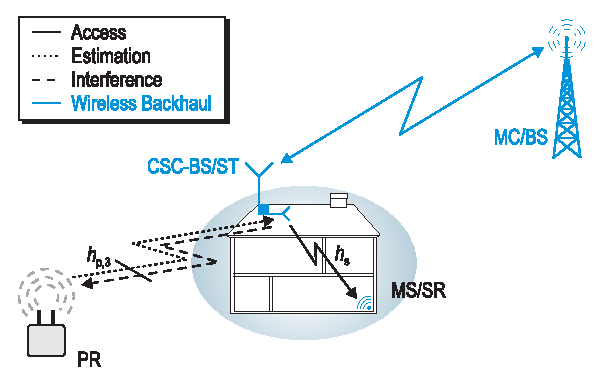
\includegraphics[width = 0.85 \columnwidth]{../kapitel06/figures/CR_Scenario_Underlay_gruen} 
				};
			\end{tikzpicture}	
			\end{overlayarea}
			\centering
			\begin{tikzpicture}[scale=1]
				\node[anchor=south west,inner sep=0] (image) at (0,0)
				{
					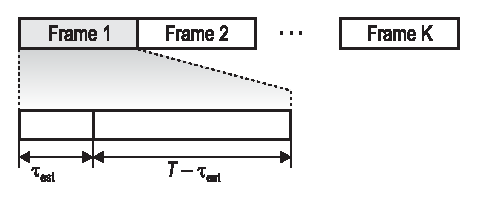
\includegraphics[width = 0.85 \columnwidth]{../kapitel06/figures/Frame_Structure_grau_U} 
				};
			\end{tikzpicture}	
		\end{column}
	\end{columns}
\end{frame}


\subsection{Validation}
%%%%%%%%%%%%%%%%%%%%%%%%%%%%%%%%%%%%%%%%%%%%%%%%%%%%%%%%%%%%%%%%%%%%%%%%%%%%%%%%
\begin{frame}[c]{Validation}
%%%%%%%%%%%%%%%%%%%%%%%%%%%%%%%%%%%%%%%%%%%%%%%%%%%%%%%%%%%%%%%%%%%%%%%%%%%%%%%%
	\begin{columns}
		\begin{column}{0.45\columnwidth}
			\fs{7}{8}
			\centering
             	        \resizebox{.95 \columnwidth}{!}{%
			\begin{tikzpicture}[scale=1]
				\node[anchor=south west,inner sep=0] (image) at (0,0)
            		    	{
               		        	\includegraphics[width=\figscale]{../kapitel06/figures/ValidationSetUp.ps}
                		};

        	        \begin{scope}[x={(image.south east)},y={(image.north west)}]
               	 	\node[draw, fill=gray!10,font=\scriptsize] at (0.49,0.765) {Signal Generator (PR)};
               	 	\node[draw, fill=gray!10,font=\scriptsize] at (0.52,0.6) {Coaxial Cable $\phpth$};

             	        \node[draw, fill=gray!10,font=\scriptsize] at (0.49,0.09) {Host Computer};
               	        \node[draw, fill=gray!10,font=\scriptsize, text width = 1cm, align = center] at (0.13,0.11) {SDR platform (ST)};
                	\node[draw, fill=gray!10,font=\scriptsize, text width = 1cm, align = center] at (0.87,0.24) {USB Interface};
                	%\draw[help lines,xstep=.1,ystep=.1] (0,0) grid (1,1);
                	%\foreach \x in {0,1,...,9} { \node [anchor=north] at (\x/10,0) {0.\x}; }
                	%\foreach \y in {0,1,...,9} { \node [anchor=east] at (0,\y/10) {0.\y}; }
                	\end{scope}
			\end{tikzpicture}
		}
		\end{column}
		%\begin{column}{0.5\columnwidth}
		%\end{column}
	\end{columns}
\end{frame}


%%%%%%%%%%%%%%%%%%%%%%%%%%%%%%%%%%%%%%%%%%%%%%%%%%%%%%%%%%%%%%%%%%%%%%%%%%%%%%%%
\begin{frame}[c]{Validation}
%%%%%%%%%%%%%%%%%%%%%%%%%%%%%%%%%%%%%%%%%%%%%%%%%%%%%%%%%%%%%%%%%%%%%%%%%%%%%%%%
	\begin{columns}
		\begin{column}{0.45\columnwidth}
			\fs{7}{8}
			\centering
             	        \resizebox{.95 \columnwidth}{!}{%
				% This file is generated by the MATLAB m-file laprint.m. It can be included
% into LaTeX documents using the packages graphicx, color and psfrag.
% It is accompanied by a postscript file. A sample LaTeX file is:
%    \documentclass{article}\usepackage{graphicx,color,psfrag}
%    \begin{document}% This file is generated by the MATLAB m-file laprint.m. It can be included
% into LaTeX documents using the packages graphicx, color and psfrag.
% It is accompanied by a postscript file. A sample LaTeX file is:
%    \documentclass{article}\usepackage{graphicx,color,psfrag}
%    \begin{document}% This file is generated by the MATLAB m-file laprint.m. It can be included
% into LaTeX documents using the packages graphicx, color and psfrag.
% It is accompanied by a postscript file. A sample LaTeX file is:
%    \documentclass{article}\usepackage{graphicx,color,psfrag}
%    \begin{document}\input{P_PR_Rx}\end{document}
% See http://www.mathworks.de/matlabcentral/fileexchange/loadFile.do?objectId=4638
% for recent versions of laprint.m.
%
% created by:           LaPrint version 3.16 (13.9.2004)
% created on:           21-Mar-2016 13:19:59
% eps bounding box:     16 cm x 12.1449 cm
% comment:              
%
%\begin{psfrags}%
%\psfragscanon%
%
% text strings:
\psfrag{s05}[t][t]{\fontsize{8}{12}\fontseries{m}\mathversion{normal}\fontshape{n}\selectfont \color[rgb]{0.15,0.15,0.15}\setlength{\tabcolsep}{0pt}\begin{tabular}{c}$\eprcvdpr$ = [dBm]\end{tabular}}%
\psfrag{s06}[b][b]{\fontsize{8}{12}\fontseries{m}\mathversion{normal}\fontshape{n}\selectfont \color[rgb]{0,0,0}\setlength{\tabcolsep}{0pt}\begin{tabular}{c}pdf\end{tabular}}%
\psfrag{s10}[][]{\fontsize{10}{15}\fontseries{m}\mathversion{normal}\fontshape{n}\selectfont \color[rgb]{0,0,0}\setlength{\tabcolsep}{0pt}\begin{tabular}{c} \end{tabular}}%
\psfrag{s11}[][]{\fontsize{10}{15}\fontseries{m}\mathversion{normal}\fontshape{n}\selectfont \color[rgb]{0,0,0}\setlength{\tabcolsep}{0pt}\begin{tabular}{c} \end{tabular}}%
%\psfrag{s12}[l][l]{\fontsize{8}{12}\fontseries{m}\mathversion{normal}\fontshape{n}\selectfont \color[rgb]{0,0,0}(\ref{eq_HVD:dpp})}%
\psfrag{s13}[l][l]{\fontsize{8}{12}\fontseries{m}\mathversion{normal}\fontshape{n}\selectfont \color[rgb]{0,0,0}Empirical}%
\psfrag{s14}[l][l]{\fontsize{8}{12}\fontseries{m}\mathversion{normal}\fontshape{n}\selectfont \color[rgb]{0,0,0}(\ref{eq_HVD:dpp})}%
%
% axes font properties:
\fontsize{8}{12}\fontseries{m}\mathversion{normal}%
\fontshape{n}\selectfont%
%
% xticklabels:
\psfrag{x01}[t][t]{0.8}%
\psfrag{x02}[t][t]{0.85}%
\psfrag{x03}[t][t]{0.9}%
\psfrag{x04}[t][t]{0.95}%
\psfrag{x05}[t][t]{1}%
\psfrag{x06}[t][t]{1.05}%
\psfrag{x07}[t][t]{1.1}%
\psfrag{x08}[t][t]{1.15}%
\psfrag{x09}[t][t]{1.2}%
\psfrag{x10}[t][t]{\shortstack{1.25\\$\times 10^{-11}\ $}}%
%
% yticklabels:
\psfrag{v01}[r][r]{0}%
\psfrag{v02}[r][r]{1}%
\psfrag{v03}[r][r]{2}%
\psfrag{v04}[r][r]{3}%
\psfrag{v05}[r][r]{4}%
\psfrag{v06}[r][r]{5}%
\psfrag{v07}[r][r]{6}%
\psfrag{v08}[r][r]{7}%
\psfrag{v09}[r][r]{8}%
\psfrag{v10}[r][r]{9}%
\psfrag{v11}[r][r]{10}%
\psfrag{ypower2}[Bl][Bl]{$\times 10^{11}$}%
%
% Figure:
%\resizebox{8cm}{!}{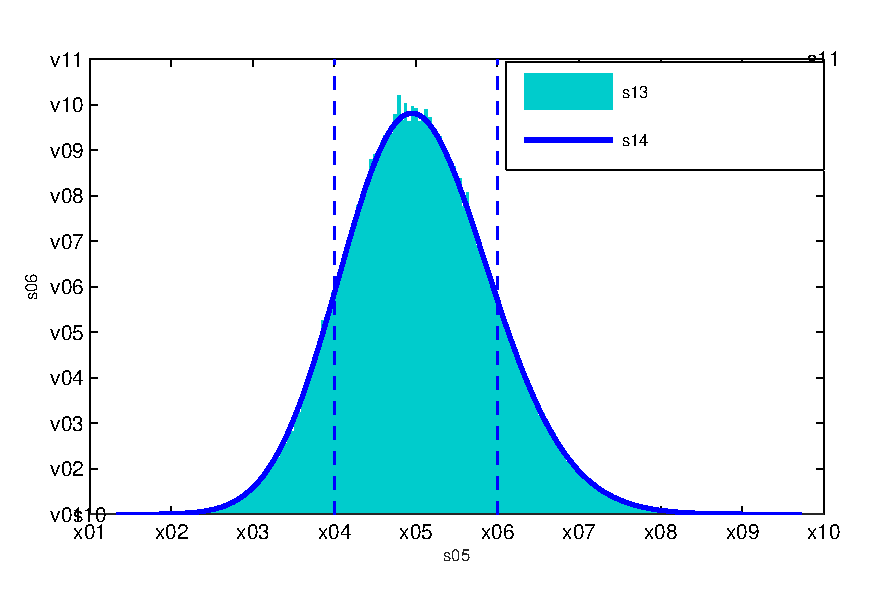
\includegraphics{P_PR_Rx.eps}}%
%\end{psfrags}%
%
% End P_PR_Rx.tex
\end{document}
% See http://www.mathworks.de/matlabcentral/fileexchange/loadFile.do?objectId=4638
% for recent versions of laprint.m.
%
% created by:           LaPrint version 3.16 (13.9.2004)
% created on:           21-Mar-2016 13:19:59
% eps bounding box:     16 cm x 12.1449 cm
% comment:              
%
%\begin{psfrags}%
%\psfragscanon%
%
% text strings:
\psfrag{s05}[t][t]{\fontsize{8}{12}\fontseries{m}\mathversion{normal}\fontshape{n}\selectfont \color[rgb]{0.15,0.15,0.15}\setlength{\tabcolsep}{0pt}\begin{tabular}{c}$\eprcvdpr$ = [dBm]\end{tabular}}%
\psfrag{s06}[b][b]{\fontsize{8}{12}\fontseries{m}\mathversion{normal}\fontshape{n}\selectfont \color[rgb]{0,0,0}\setlength{\tabcolsep}{0pt}\begin{tabular}{c}pdf\end{tabular}}%
\psfrag{s10}[][]{\fontsize{10}{15}\fontseries{m}\mathversion{normal}\fontshape{n}\selectfont \color[rgb]{0,0,0}\setlength{\tabcolsep}{0pt}\begin{tabular}{c} \end{tabular}}%
\psfrag{s11}[][]{\fontsize{10}{15}\fontseries{m}\mathversion{normal}\fontshape{n}\selectfont \color[rgb]{0,0,0}\setlength{\tabcolsep}{0pt}\begin{tabular}{c} \end{tabular}}%
%\psfrag{s12}[l][l]{\fontsize{8}{12}\fontseries{m}\mathversion{normal}\fontshape{n}\selectfont \color[rgb]{0,0,0}(\ref{eq_HVD:dpp})}%
\psfrag{s13}[l][l]{\fontsize{8}{12}\fontseries{m}\mathversion{normal}\fontshape{n}\selectfont \color[rgb]{0,0,0}Empirical}%
\psfrag{s14}[l][l]{\fontsize{8}{12}\fontseries{m}\mathversion{normal}\fontshape{n}\selectfont \color[rgb]{0,0,0}(\ref{eq_HVD:dpp})}%
%
% axes font properties:
\fontsize{8}{12}\fontseries{m}\mathversion{normal}%
\fontshape{n}\selectfont%
%
% xticklabels:
\psfrag{x01}[t][t]{0.8}%
\psfrag{x02}[t][t]{0.85}%
\psfrag{x03}[t][t]{0.9}%
\psfrag{x04}[t][t]{0.95}%
\psfrag{x05}[t][t]{1}%
\psfrag{x06}[t][t]{1.05}%
\psfrag{x07}[t][t]{1.1}%
\psfrag{x08}[t][t]{1.15}%
\psfrag{x09}[t][t]{1.2}%
\psfrag{x10}[t][t]{\shortstack{1.25\\$\times 10^{-11}\ $}}%
%
% yticklabels:
\psfrag{v01}[r][r]{0}%
\psfrag{v02}[r][r]{1}%
\psfrag{v03}[r][r]{2}%
\psfrag{v04}[r][r]{3}%
\psfrag{v05}[r][r]{4}%
\psfrag{v06}[r][r]{5}%
\psfrag{v07}[r][r]{6}%
\psfrag{v08}[r][r]{7}%
\psfrag{v09}[r][r]{8}%
\psfrag{v10}[r][r]{9}%
\psfrag{v11}[r][r]{10}%
\psfrag{ypower2}[Bl][Bl]{$\times 10^{11}$}%
%
% Figure:
%\resizebox{8cm}{!}{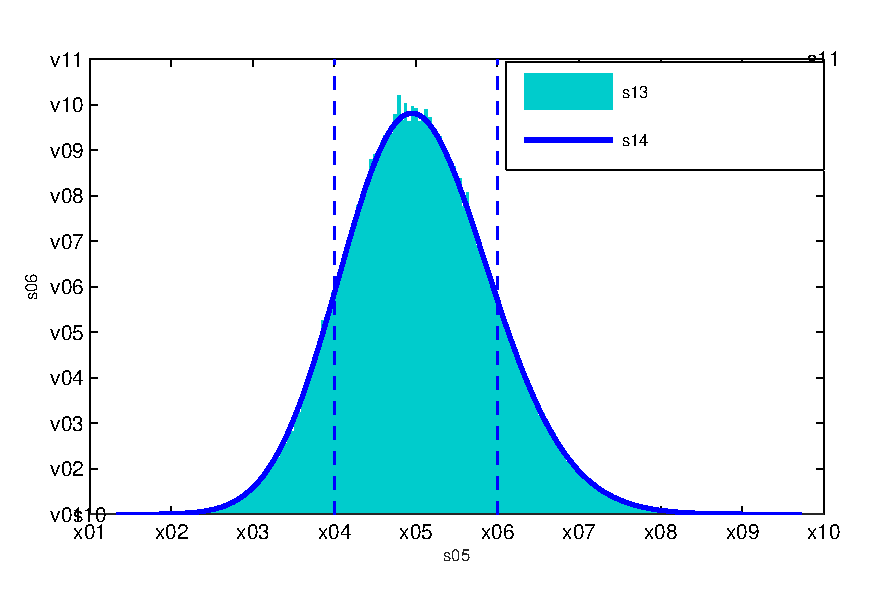
\includegraphics{P_PR_Rx.eps}}%
%\end{psfrags}%
%
% End P_PR_Rx.tex
\end{document}
% See http://www.mathworks.de/matlabcentral/fileexchange/loadFile.do?objectId=4638
% for recent versions of laprint.m.
%
% created by:           LaPrint version 3.16 (13.9.2004)
% created on:           21-Mar-2016 13:19:59
% eps bounding box:     16 cm x 12.1449 cm
% comment:              
%
%\begin{psfrags}%
%\psfragscanon%
%
% text strings:
\psfrag{s05}[t][t]{\fontsize{8}{12}\fontseries{m}\mathversion{normal}\fontshape{n}\selectfont \color[rgb]{0.15,0.15,0.15}\setlength{\tabcolsep}{0pt}\begin{tabular}{c}$\eprcvdpr$ = [dBm]\end{tabular}}%
\psfrag{s06}[b][b]{\fontsize{8}{12}\fontseries{m}\mathversion{normal}\fontshape{n}\selectfont \color[rgb]{0,0,0}\setlength{\tabcolsep}{0pt}\begin{tabular}{c}pdf\end{tabular}}%
\psfrag{s10}[][]{\fontsize{10}{15}\fontseries{m}\mathversion{normal}\fontshape{n}\selectfont \color[rgb]{0,0,0}\setlength{\tabcolsep}{0pt}\begin{tabular}{c} \end{tabular}}%
\psfrag{s11}[][]{\fontsize{10}{15}\fontseries{m}\mathversion{normal}\fontshape{n}\selectfont \color[rgb]{0,0,0}\setlength{\tabcolsep}{0pt}\begin{tabular}{c} \end{tabular}}%
%\psfrag{s12}[l][l]{\fontsize{8}{12}\fontseries{m}\mathversion{normal}\fontshape{n}\selectfont \color[rgb]{0,0,0}(\ref{eq_HVD:dpp})}%
\psfrag{s13}[l][l]{\fontsize{8}{12}\fontseries{m}\mathversion{normal}\fontshape{n}\selectfont \color[rgb]{0,0,0}Empirical}%
\psfrag{s14}[l][l]{\fontsize{8}{12}\fontseries{m}\mathversion{normal}\fontshape{n}\selectfont \color[rgb]{0,0,0}(\ref{eq_HVD:dpp})}%
%
% axes font properties:
\fontsize{8}{12}\fontseries{m}\mathversion{normal}%
\fontshape{n}\selectfont%
%
% xticklabels:
\psfrag{x01}[t][t]{0.8}%
\psfrag{x02}[t][t]{0.85}%
\psfrag{x03}[t][t]{0.9}%
\psfrag{x04}[t][t]{0.95}%
\psfrag{x05}[t][t]{1}%
\psfrag{x06}[t][t]{1.05}%
\psfrag{x07}[t][t]{1.1}%
\psfrag{x08}[t][t]{1.15}%
\psfrag{x09}[t][t]{1.2}%
\psfrag{x10}[t][t]{\shortstack{1.25\\$\times 10^{-11}\ $}}%
%
% yticklabels:
\psfrag{v01}[r][r]{0}%
\psfrag{v02}[r][r]{1}%
\psfrag{v03}[r][r]{2}%
\psfrag{v04}[r][r]{3}%
\psfrag{v05}[r][r]{4}%
\psfrag{v06}[r][r]{5}%
\psfrag{v07}[r][r]{6}%
\psfrag{v08}[r][r]{7}%
\psfrag{v09}[r][r]{8}%
\psfrag{v10}[r][r]{9}%
\psfrag{v11}[r][r]{10}%
\psfrag{ypower2}[Bl][Bl]{$\times 10^{11}$}%
%
% Figure:
%\resizebox{8cm}{!}{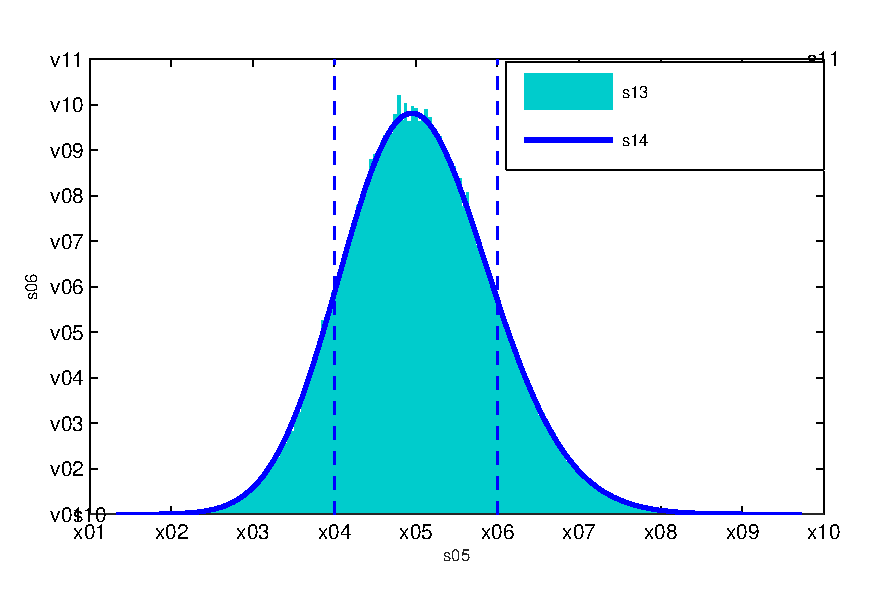
\includegraphics{P_PR_Rx.eps}}%
%\end{psfrags}%
%
% End P_PR_Rx.tex

      		  		\begin{tikzpicture}[scale=1]
                		\node[anchor=south west,inner sep=0] (image) at (0,0)
          		        {
                        		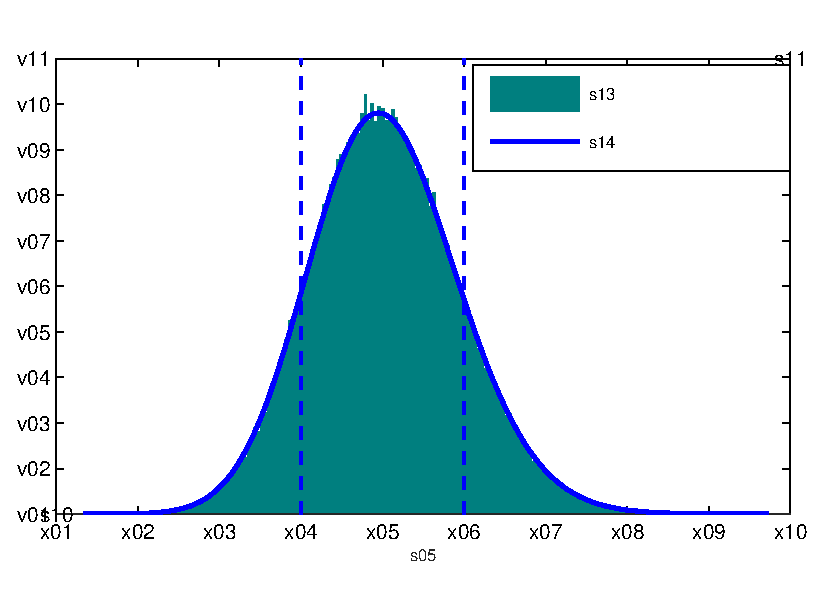
\includegraphics[width=\figscale]{../kapitel06/figures/P_PR_Rx}
            		        };

            		        \begin{scope}[x={(image.south east)},y={(image.north west)}]
           		        \node[above, font=\footnotesize] at (0.16,0.93) {$ \times 10^{-11}$};

            		        \draw[black,thick,<-] (0.577,0.57) --  node[above, font=\footnotesize] {$\ite (1 + \acc)$} (0.777,0.57);
                		\draw[black,thick,<-] (0.379,0.57) --  node[above, font=\footnotesize] {$\ite (1 - \acc)$} (0.179,0.57);
            		        %\draw[help lines,xstep=.1,ystep=.1] (0,0) grid (1,1);
              		        %\foreach \x in {0,1,...,9} { \node [anchor=north] at (\x/10,0) {0.\x}; }
                		%\foreach \y in {0,1,...,9} { \node [anchor=east] at (0,\y/10) {0.\y}; }
                		\end{scope}
      		  		\end{tikzpicture}
			}
			\vspace{2mm}	
				
             	        \resizebox{.95 \columnwidth}{!}{%
				% This file is generated by the MATLAB m-file laprint.m. It can be included
% into LaTeX documents using the packages graphicx, color and psfrag.
% It is accompanied by a postscript file. A sample LaTeX file is:
%    \documentclass{article}\usepackage{graphicx,color,psfrag}
%    \begin{document}% This file is generated by the MATLAB m-file laprint.m. It can be included
% into LaTeX documents using the packages graphicx, color and psfrag.
% It is accompanied by a postscript file. A sample LaTeX file is:
%    \documentclass{article}\usepackage{graphicx,color,psfrag}
%    \begin{document}% This file is generated by the MATLAB m-file laprint.m. It can be included
% into LaTeX documents using the packages graphicx, color and psfrag.
% It is accompanied by a postscript file. A sample LaTeX file is:
%    \documentclass{article}\usepackage{graphicx,color,psfrag}
%    \begin{document}\input{R_s}\end{document}
% See http://www.mathworks.de/matlabcentral/fileexchange/loadFile.do?objectId=4638
% for recent versions of laprint.m.
%
% created by:           LaPrint version 3.16 (13.9.2004)
% created on:           21-Mar-2016 13:20:00
% eps bounding box:     16 cm x 12.1449 cm
% comment:              
%
%\begin{psfrags}%
%\psfragscanon%
%
% text strings:
\psfrag{s05}[t][t]{\fontsize{8}{12}\fontseries{m}\mathversion{normal}\fontshape{n}\selectfont \color[rgb]{0.15,0.15,0.15}\setlength{\tabcolsep}{0pt}\begin{tabular}{c}$\ers$ [bits/sec/Hz]\end{tabular}}%
\psfrag{s06}[b][b]{\fontsize{8}{12}\fontseries{m}\mathversion{normal}\fontshape{n}\selectfont \color[rgb]{0,0,0}\setlength{\tabcolsep}{0pt}\begin{tabular}{c}pdf\end{tabular}}%
\psfrag{s10}[][]{\fontsize{10}{15}\fontseries{m}\mathversion{normal}\fontshape{n}\selectfont \color[rgb]{0,0,0}\setlength{\tabcolsep}{0pt}\begin{tabular}{c} \end{tabular}}%
\psfrag{s11}[][]{\fontsize{10}{15}\fontseries{m}\mathversion{normal}\fontshape{n}\selectfont \color[rgb]{0,0,0}\setlength{\tabcolsep}{0pt}\begin{tabular}{c} \end{tabular}}%
%\psfrag{s12}[l][l]{\fontsize{8}{12}\fontseries{m}\mathversion{normal}\fontshape{n}\selectfont \color[rgb]{0,0,0}(\ref{eq_HVD:drs})}%
\psfrag{s13}[l][l]{\fontsize{8}{12}\fontseries{m}\mathversion{normal}\fontshape{n}\selectfont \color[rgb]{0,0,0}Empirical}%
\psfrag{s14}[l][l]{\fontsize{8}{12}\fontseries{m}\mathversion{normal}\fontshape{n}\selectfont \color[rgb]{0,0,0}Theoretical}%
%
% axes font properties:
\fontsize{8}{12}\fontseries{m}\mathversion{normal}%
\fontshape{n}\selectfont%
%
% xticklabels:
\psfrag{x01}[t][t]{6.6}%
\psfrag{x02}[t][t]{6.7}%
\psfrag{x03}[t][t]{6.8}%
\psfrag{x04}[t][t]{6.9}%
\psfrag{x05}[t][t]{7}%
\psfrag{x06}[t][t]{7.1}%
\psfrag{x07}[t][t]{7.2}%
\psfrag{x08}[t][t]{7.3}%
\psfrag{x09}[t][t]{7.4}%
%
% yticklabels:
\psfrag{v01}[r][r]{0}%
\psfrag{v02}[r][r]{1}%
\psfrag{v03}[r][r]{2}%
\psfrag{v04}[r][r]{3}%
\psfrag{v05}[r][r]{4}%
\psfrag{v06}[r][r]{5}%
\psfrag{v07}[r][r]{6}%
\psfrag{v08}[r][r]{7}%
%
% Figure:
%\resizebox{8cm}{!}{\includegraphics{R_s.eps}}%
%\end{psfrags}%
%
% End R_s.tex
\end{document}
% See http://www.mathworks.de/matlabcentral/fileexchange/loadFile.do?objectId=4638
% for recent versions of laprint.m.
%
% created by:           LaPrint version 3.16 (13.9.2004)
% created on:           21-Mar-2016 13:20:00
% eps bounding box:     16 cm x 12.1449 cm
% comment:              
%
%\begin{psfrags}%
%\psfragscanon%
%
% text strings:
\psfrag{s05}[t][t]{\fontsize{8}{12}\fontseries{m}\mathversion{normal}\fontshape{n}\selectfont \color[rgb]{0.15,0.15,0.15}\setlength{\tabcolsep}{0pt}\begin{tabular}{c}$\ers$ [bits/sec/Hz]\end{tabular}}%
\psfrag{s06}[b][b]{\fontsize{8}{12}\fontseries{m}\mathversion{normal}\fontshape{n}\selectfont \color[rgb]{0,0,0}\setlength{\tabcolsep}{0pt}\begin{tabular}{c}pdf\end{tabular}}%
\psfrag{s10}[][]{\fontsize{10}{15}\fontseries{m}\mathversion{normal}\fontshape{n}\selectfont \color[rgb]{0,0,0}\setlength{\tabcolsep}{0pt}\begin{tabular}{c} \end{tabular}}%
\psfrag{s11}[][]{\fontsize{10}{15}\fontseries{m}\mathversion{normal}\fontshape{n}\selectfont \color[rgb]{0,0,0}\setlength{\tabcolsep}{0pt}\begin{tabular}{c} \end{tabular}}%
%\psfrag{s12}[l][l]{\fontsize{8}{12}\fontseries{m}\mathversion{normal}\fontshape{n}\selectfont \color[rgb]{0,0,0}(\ref{eq_HVD:drs})}%
\psfrag{s13}[l][l]{\fontsize{8}{12}\fontseries{m}\mathversion{normal}\fontshape{n}\selectfont \color[rgb]{0,0,0}Empirical}%
\psfrag{s14}[l][l]{\fontsize{8}{12}\fontseries{m}\mathversion{normal}\fontshape{n}\selectfont \color[rgb]{0,0,0}Theoretical}%
%
% axes font properties:
\fontsize{8}{12}\fontseries{m}\mathversion{normal}%
\fontshape{n}\selectfont%
%
% xticklabels:
\psfrag{x01}[t][t]{6.6}%
\psfrag{x02}[t][t]{6.7}%
\psfrag{x03}[t][t]{6.8}%
\psfrag{x04}[t][t]{6.9}%
\psfrag{x05}[t][t]{7}%
\psfrag{x06}[t][t]{7.1}%
\psfrag{x07}[t][t]{7.2}%
\psfrag{x08}[t][t]{7.3}%
\psfrag{x09}[t][t]{7.4}%
%
% yticklabels:
\psfrag{v01}[r][r]{0}%
\psfrag{v02}[r][r]{1}%
\psfrag{v03}[r][r]{2}%
\psfrag{v04}[r][r]{3}%
\psfrag{v05}[r][r]{4}%
\psfrag{v06}[r][r]{5}%
\psfrag{v07}[r][r]{6}%
\psfrag{v08}[r][r]{7}%
%
% Figure:
%\resizebox{8cm}{!}{\includegraphics{R_s.eps}}%
%\end{psfrags}%
%
% End R_s.tex
\end{document}
% See http://www.mathworks.de/matlabcentral/fileexchange/loadFile.do?objectId=4638
% for recent versions of laprint.m.
%
% created by:           LaPrint version 3.16 (13.9.2004)
% created on:           18-Mar-2016 14:57:26
% eps bounding box:     16 cm x 11.8592 cm
% comment:              
%
%\begin{psfrags}%
%\psfragscanon%
%
% text strings:
\psfrag{s05}[t][t]{\fontsize{8}{12}\fontseries{m}\mathversion{normal}\fontshape{n}\selectfont \color[rgb]{0.15,0.15,0.15}\setlength{\tabcolsep}{0pt}\begin{tabular}{c}$\ers$\end{tabular}}%
\psfrag{s10}[][]{\fontsize{10}{15}\fontseries{m}\mathversion{normal}\fontshape{n}\selectfont \color[rgb]{0,0,0}\setlength{\tabcolsep}{0pt}\begin{tabular}{c} \end{tabular}}%
\psfrag{s11}[][]{\fontsize{10}{15}\fontseries{m}\mathversion{normal}\fontshape{n}\selectfont \color[rgb]{0,0,0}\setlength{\tabcolsep}{0pt}\begin{tabular}{c} \end{tabular}}%
\psfrag{s12}[l][l]{\fontsize{8}{12}\fontseries{m}\mathversion{normal}\fontshape{n}\selectfont \color[rgb]{0,0,0}Theoretical}%
\psfrag{s13}[l][l]{\fontsize{8}{12}\fontseries{m}\mathversion{normal}\fontshape{n}\selectfont \color[rgb]{0,0,0}Empirical}%
\psfrag{s14}[l][l]{\fontsize{8}{12}\fontseries{m}\mathversion{normal}\fontshape{n}\selectfont \color[rgb]{0,0,0}Theoretical}%
%
% axes font properties:
\fontsize{8}{12}\fontseries{m}\mathversion{normal}%
\fontshape{n}\selectfont%
%
% xticklabels:
\psfrag{x01}[t][t]{6.6}%
\psfrag{x02}[t][t]{6.7}%
\psfrag{x03}[t][t]{6.8}%
\psfrag{x04}[t][t]{6.9}%
\psfrag{x05}[t][t]{7}%
\psfrag{x06}[t][t]{7.1}%
\psfrag{x07}[t][t]{7.2}%
\psfrag{x08}[t][t]{7.3}%
\psfrag{x09}[t][t]{7.4}%
%
% yticklabels:
\psfrag{v01}[r][r]{0}%
\psfrag{v02}[r][r]{1}%
\psfrag{v03}[r][r]{2}%
\psfrag{v04}[r][r]{3}%
\psfrag{v05}[r][r]{4}%
\psfrag{v06}[r][r]{5}%
\psfrag{v07}[r][r]{6}%
\psfrag{v08}[r][r]{7}%
%
% Figure:
%\resizebox{8cm}{!}{\includegraphics{R_s.eps}}%
%\end{psfrags}%
%
% End R_s.tex

			        \includegraphics[width=\figscale]{../kapitel06/figures/R_s}%
			}
		\end{column}
		\begin{column}{0.55\columnwidth}
		\fs{7}{8}
		\begin{overlayarea}{\textwidth}{3.1cm}
			\vspace{2mm}	
		\begin{center}
		\centering
		\begin{tabular}{c||c}
                	\rowcolor{kit-green30}
			Parameter & Value \\ \hline \hline
                	$\snrrcvdu$ & \SI{22}{dB} \\
                	$N$ & 100 \\
                	$\test$ & \SI{2}{ms}\\
                	$\ite$ & \SI{-110}{dBm}\\
                	$T$ & \SI{100}{ms}\\
               		$\pgs$ & 1 \\
                	$\npp$ & $\SI{-96.74}{dBm}$\\ \hline
        	\end{tabular}
		\end{center}
		\end{overlayarea}
		\resizebox{.95 \columnwidth}{!}{%
		\centering
			% This file is generated by the MATLAB m-file laprint.m. It can be included
% into LaTeX documents using the packages graphicx, color and psfrag.
% It is accompanied by a postscript file. A sample LaTeX file is:
%    \documentclass{article}\usepackage{graphicx,color,psfrag}
%    \begin{document}% This file is generated by the MATLAB m-file laprint.m. It can be included
% into LaTeX documents using the packages graphicx, color and psfrag.
% It is accompanied by a postscript file. A sample LaTeX file is:
%    \documentclass{article}\usepackage{graphicx,color,psfrag}
%    \begin{document}% This file is generated by the MATLAB m-file laprint.m. It can be included
% into LaTeX documents using the packages graphicx, color and psfrag.
% It is accompanied by a postscript file. A sample LaTeX file is:
%    \documentclass{article}\usepackage{graphicx,color,psfrag}
%    \begin{document}\input{ETT}\end{document}
% See http://www.mathworks.de/matlabcentral/fileexchange/loadFile.do?objectId=4638
% for recent versions of laprint.m.
%
% created by:           LaPrint version 3.16 (13.9.2004)
% created on:           23-Mar-2016 13:43:56
% eps bounding box:     16 cm x 12 cm
% comment:              
%
%\begin{psfrags}%
%\psfragscanon%
%
% text strings:
\psfrag{s06}[t][t]{\fontsize{8}{12}\fontseries{m}\mathversion{normal}\fontshape{n}\selectfont \color[rgb]{0,0,0}\setlength{\tabcolsep}{0pt}\begin{tabular}{c}$\test = [\SI{}{ms}]$\end{tabular}}%
\psfrag{s07}[b][b]{\fontsize{8}{12}\fontseries{m}\mathversion{normal}\fontshape{n}\selectfont \color[rgb]{0,0,0}\setlength{\tabcolsep}{0pt}\begin{tabular}{c}$\e{\ers}{\ers}  = [\SI{}{bits/s/Hz}]$\end{tabular}}%
\psfrag{s11}[][]{\fontsize{10}{15}\fontseries{m}\mathversion{normal}\fontshape{n}\selectfont \color[rgb]{0,0,0}\setlength{\tabcolsep}{0pt}\begin{tabular}{c} \end{tabular}}%
\psfrag{s12}[][]{\fontsize{10}{15}\fontseries{m}\mathversion{normal}\fontshape{n}\selectfont \color[rgb]{0,0,0}\setlength{\tabcolsep}{0pt}\begin{tabular}{c} \end{tabular}}%
\psfrag{s14}[t][t]{\fontsize{8}{12}\fontseries{m}\mathversion{normal}\fontshape{n}\selectfont \color[rgb]{0,0,0}\setlength{\tabcolsep}{0pt}\begin{tabular}{c}$\pco$\end{tabular}}%
\psfrag{s18}[l][l]{\fontsize{8}{12}\fontseries{m}\mathversion{normal}\fontshape{n}\selectfont \color[rgb]{0,0,0}Empirical}%
\psfrag{s19}[l][l]{\fontsize{8}{12}\fontseries{m}\mathversion{normal}\fontshape{n}\selectfont \color[rgb]{0,0,0}$\e{\ers}{\ers}$]}%
\psfrag{s20}[l][l]{\fontsize{8}{12}\fontseries{m}\mathversion{normal}\fontshape{n}\selectfont \color[rgb]{0,0,0}$\pco$}%
\psfrag{s21}[l][l]{\fontsize{8}{12}\fontseries{m}\mathversion{normal}\fontshape{n}\selectfont \color[rgb]{0,0,0}Empirical}%
%
% axes font properties:
\fontsize{8}{12}\fontseries{m}\mathversion{normal}%
\fontshape{n}\selectfont%
%
% xticklabels:
\psfrag{x01}[t][t]{0}%
\psfrag{x02}[t][t]{0.5}%
\psfrag{x03}[t][t]{1}%
\psfrag{x04}[t][t]{1.5}%
\psfrag{x05}[t][t]{2}%
\psfrag{x06}[t][t]{2.5}%
\psfrag{x07}[t][t]{0}%
\psfrag{x08}[t][t]{0.5}%
\psfrag{x09}[t][t]{1}%
\psfrag{x10}[t][t]{1.5}%
\psfrag{x11}[t][t]{2}%
\psfrag{x12}[t][t]{2.5}%
%
% yticklabels:
\psfrag{v01}[l][l]{0.50}%
\psfrag{v02}[l][l]{0.60}%
\psfrag{v03}[l][l]{0.70}%
\psfrag{v04}[l][l]{0.80}%
\psfrag{v05}[l][l]{0.90}%
\psfrag{v06}[l][l]{1.00}%
\psfrag{v07}[l][l]{}%
\psfrag{v08}[r][r]{6.89}%
\psfrag{v09}[r][r]{6.93}%
\psfrag{v10}[r][r]{6.96}%
\psfrag{v11}[r][r]{7.00}%
\psfrag{v12}[r][r]{7.04}%
\psfrag{v13}[r][r]{7.07}%
\psfrag{v14}[r][r]{}%
%
% Figure:
%\resizebox{8cm}{!}{\includegraphics{ETT.eps}}%
%\end{psfrags}%
%
% End ETT.tex
\end{document}
% See http://www.mathworks.de/matlabcentral/fileexchange/loadFile.do?objectId=4638
% for recent versions of laprint.m.
%
% created by:           LaPrint version 3.16 (13.9.2004)
% created on:           23-Mar-2016 13:43:56
% eps bounding box:     16 cm x 12 cm
% comment:              
%
%\begin{psfrags}%
%\psfragscanon%
%
% text strings:
\psfrag{s06}[t][t]{\fontsize{8}{12}\fontseries{m}\mathversion{normal}\fontshape{n}\selectfont \color[rgb]{0,0,0}\setlength{\tabcolsep}{0pt}\begin{tabular}{c}$\test = [\SI{}{ms}]$\end{tabular}}%
\psfrag{s07}[b][b]{\fontsize{8}{12}\fontseries{m}\mathversion{normal}\fontshape{n}\selectfont \color[rgb]{0,0,0}\setlength{\tabcolsep}{0pt}\begin{tabular}{c}$\e{\ers}{\ers}  = [\SI{}{bits/s/Hz}]$\end{tabular}}%
\psfrag{s11}[][]{\fontsize{10}{15}\fontseries{m}\mathversion{normal}\fontshape{n}\selectfont \color[rgb]{0,0,0}\setlength{\tabcolsep}{0pt}\begin{tabular}{c} \end{tabular}}%
\psfrag{s12}[][]{\fontsize{10}{15}\fontseries{m}\mathversion{normal}\fontshape{n}\selectfont \color[rgb]{0,0,0}\setlength{\tabcolsep}{0pt}\begin{tabular}{c} \end{tabular}}%
\psfrag{s14}[t][t]{\fontsize{8}{12}\fontseries{m}\mathversion{normal}\fontshape{n}\selectfont \color[rgb]{0,0,0}\setlength{\tabcolsep}{0pt}\begin{tabular}{c}$\pco$\end{tabular}}%
\psfrag{s18}[l][l]{\fontsize{8}{12}\fontseries{m}\mathversion{normal}\fontshape{n}\selectfont \color[rgb]{0,0,0}Empirical}%
\psfrag{s19}[l][l]{\fontsize{8}{12}\fontseries{m}\mathversion{normal}\fontshape{n}\selectfont \color[rgb]{0,0,0}$\e{\ers}{\ers}$]}%
\psfrag{s20}[l][l]{\fontsize{8}{12}\fontseries{m}\mathversion{normal}\fontshape{n}\selectfont \color[rgb]{0,0,0}$\pco$}%
\psfrag{s21}[l][l]{\fontsize{8}{12}\fontseries{m}\mathversion{normal}\fontshape{n}\selectfont \color[rgb]{0,0,0}Empirical}%
%
% axes font properties:
\fontsize{8}{12}\fontseries{m}\mathversion{normal}%
\fontshape{n}\selectfont%
%
% xticklabels:
\psfrag{x01}[t][t]{0}%
\psfrag{x02}[t][t]{0.5}%
\psfrag{x03}[t][t]{1}%
\psfrag{x04}[t][t]{1.5}%
\psfrag{x05}[t][t]{2}%
\psfrag{x06}[t][t]{2.5}%
\psfrag{x07}[t][t]{0}%
\psfrag{x08}[t][t]{0.5}%
\psfrag{x09}[t][t]{1}%
\psfrag{x10}[t][t]{1.5}%
\psfrag{x11}[t][t]{2}%
\psfrag{x12}[t][t]{2.5}%
%
% yticklabels:
\psfrag{v01}[l][l]{0.50}%
\psfrag{v02}[l][l]{0.60}%
\psfrag{v03}[l][l]{0.70}%
\psfrag{v04}[l][l]{0.80}%
\psfrag{v05}[l][l]{0.90}%
\psfrag{v06}[l][l]{1.00}%
\psfrag{v07}[l][l]{}%
\psfrag{v08}[r][r]{6.89}%
\psfrag{v09}[r][r]{6.93}%
\psfrag{v10}[r][r]{6.96}%
\psfrag{v11}[r][r]{7.00}%
\psfrag{v12}[r][r]{7.04}%
\psfrag{v13}[r][r]{7.07}%
\psfrag{v14}[r][r]{}%
%
% Figure:
%\resizebox{8cm}{!}{\includegraphics{ETT.eps}}%
%\end{psfrags}%
%
% End ETT.tex
\end{document}
% See http://www.mathworks.de/matlabcentral/fileexchange/loadFile.do?objectId=4638
% for recent versions of laprint.m.
%
% created by:           LaPrint version 3.16 (13.9.2004)
% created on:           23-Mar-2016 13:43:56
% eps bounding box:     16 cm x 12 cm
% comment:              
%
%\begin{psfrags}%
%\psfragscanon%
%
% text strings:
\psfrag{s06}[t][t]{\fontsize{8}{12}\fontseries{m}\mathversion{normal}\fontshape{n}\selectfont \color[rgb]{0,0,0}\setlength{\tabcolsep}{0pt}\begin{tabular}{c}$\test = [\SI{}{ms}]$\end{tabular}}%
\psfrag{s07}[b][b]{\fontsize{8}{12}\fontseries{m}\mathversion{normal}\fontshape{n}\selectfont \color[rgb]{0,0,0}\setlength{\tabcolsep}{0pt}\begin{tabular}{c}$\e{\ers}{\ers}  = [\SI{}{bits/s/Hz}]$\end{tabular}}%
\psfrag{s11}[][]{\fontsize{10}{15}\fontseries{m}\mathversion{normal}\fontshape{n}\selectfont \color[rgb]{0,0,0}\setlength{\tabcolsep}{0pt}\begin{tabular}{c} \end{tabular}}%
\psfrag{s12}[][]{\fontsize{10}{15}\fontseries{m}\mathversion{normal}\fontshape{n}\selectfont \color[rgb]{0,0,0}\setlength{\tabcolsep}{0pt}\begin{tabular}{c} \end{tabular}}%
\psfrag{s14}[t][t]{\fontsize{8}{12}\fontseries{m}\mathversion{normal}\fontshape{n}\selectfont \color[rgb]{0,0,0}\setlength{\tabcolsep}{0pt}\begin{tabular}{c}$\pco$\end{tabular}}%
\psfrag{s18}[l][l]{\fontsize{8}{12}\fontseries{m}\mathversion{normal}\fontshape{n}\selectfont \color[rgb]{0,0,0}Empirical}%
\psfrag{s19}[l][l]{\fontsize{8}{12}\fontseries{m}\mathversion{normal}\fontshape{n}\selectfont \color[rgb]{0,0,0}$\e{\ers}{\ers}$]}%
\psfrag{s20}[l][l]{\fontsize{8}{12}\fontseries{m}\mathversion{normal}\fontshape{n}\selectfont \color[rgb]{0,0,0}$\pco$}%
\psfrag{s21}[l][l]{\fontsize{8}{12}\fontseries{m}\mathversion{normal}\fontshape{n}\selectfont \color[rgb]{0,0,0}Empirical}%
%
% axes font properties:
\fontsize{8}{12}\fontseries{m}\mathversion{normal}%
\fontshape{n}\selectfont%
%
% xticklabels:
\psfrag{x01}[t][t]{0}%
\psfrag{x02}[t][t]{0.5}%
\psfrag{x03}[t][t]{1}%
\psfrag{x04}[t][t]{1.5}%
\psfrag{x05}[t][t]{2}%
\psfrag{x06}[t][t]{2.5}%
\psfrag{x07}[t][t]{0}%
\psfrag{x08}[t][t]{0.5}%
\psfrag{x09}[t][t]{1}%
\psfrag{x10}[t][t]{1.5}%
\psfrag{x11}[t][t]{2}%
\psfrag{x12}[t][t]{2.5}%
%
% yticklabels:
\psfrag{v01}[l][l]{0.50}%
\psfrag{v02}[l][l]{0.60}%
\psfrag{v03}[l][l]{0.70}%
\psfrag{v04}[l][l]{0.80}%
\psfrag{v05}[l][l]{0.90}%
\psfrag{v06}[l][l]{1.00}%
\psfrag{v07}[l][l]{}%
\psfrag{v08}[r][r]{6.89}%
\psfrag{v09}[r][r]{6.93}%
\psfrag{v10}[r][r]{6.96}%
\psfrag{v11}[r][r]{7.00}%
\psfrag{v12}[r][r]{7.04}%
\psfrag{v13}[r][r]{7.07}%
\psfrag{v14}[r][r]{}%
%
% Figure:
%\resizebox{8cm}{!}{\includegraphics{ETT.eps}}%
%\end{psfrags}%
%
% End ETT.tex

		        \begin{tikzpicture}[scale=1]
       				\node[anchor=south west,inner sep=0] (image) at (0,0)
        			{
                			\includegraphics[width=\figscale]{../kapitel06/figures/ETT}
        			};
        			\begin{scope}[x={(image.south east)},y={(image.north west)}]
        			\node[draw, fill=gray!10,font=\scriptsize] (text1) at (0.98,0.872) {$\pcod$};
        			\draw[black, ->] (text1.west) -- (0.913,0.872);

       				\node[draw, fill=gray!10,font=\scriptsize] (text2) at (0.3275,0.01) {$\ttest$};
        			\draw[black, ->] (text2.north) -- (0.3275,0.086);

        			\node[draw, fill=gray!10,font=\scriptsize] (text3) at (-0.06,0.9) {$\maxi\e{\ers}{\ers}$};
        			\draw[black, ->] (text3.south) -- (0.084,0.7);

                		%\draw[help lines,xstep=.1,ystep=.1] (0,0) grid (1,1);
                		%\foreach \x in {0,1,...,9} { \node [anchor=north] at (\x/10,0) {0.\x}; }
                		%\foreach \y in {0,1,...,9} { \node [anchor=east] at (0,\y/10) {0.\y}; }
                		\end{scope}
        		\end{tikzpicture}
			}
		\end{column}
	\end{columns}
\end{frame}

\newcommand{\anglee}{00}
\subsection{Demonstration}
%%%%%%%%%%%%%%%%%%%%%%%%%%%%%%%%%%%%%%%%%%%%%%%%%%%%%%%%%%%%%%%%%%%%%%%%%%%%%%%%
\begin{frame}[c]{Demonstration}
%%%%%%%%%%%%%%%%%%%%%%%%%%%%%%%%%%%%%%%%%%%%%%%%%%%%%%%%%%%%%%%%%%%%%%%%%%%%%%%%
		\fs{7}{8}
		\centering
             	%\resizebox{1.\columnwidth}{!}{%

		\begin{tikzpicture}[scale=1]
                	\node[anchor=south west,inner sep=0] (image) at (0,0)
                {
                        \includegraphics[width=1.0 \columnwidth, angle = \anglee]{../kapitel06/figures/BlockDiagram_Demo.ps}
                };

                \begin{scope}[x={(image.south east)},y={(image.north west)}]

                %\node[draw, fill=kit-green30, font=\tiny, rotate = \anglee, align = center] at (0.48,1.3) {Block Diagram of the Deployment Demonstrator};
                
		\node[draw, fill=kit-green30, font=\tiny, rotate = \anglee, align = center] at (0.48,1.08) {Air Interface};
                \node[draw, fill=kit-green30, font=\tiny, rotate = \anglee, align = center] at (0.391,0.037) {Primary Receiver};
                \node[draw, fill=kit-green30, font=\tiny, rotate = \anglee, align = center] at (0.5858,0.037) {Secondary Transmitter};
                \node[draw, fill=kit-green30, font=\tiny, rotate = 90, align = center] at (0.986,0.97) {SDR Interface};
                \node[draw, fill=kit-green30, font=\tiny, rotate = 90, align = center] at (0.986,0.592) {Host Interface};
		
			% Transmit and receive signals  
                \node[draw=none, font=\tiny, rotate = \anglee, align = center] at (0.27,0.97) {Rx Signal};
                \node[draw=none, font=\tiny, rotate = \anglee, align = center] at (0.27,0.879) {Tx Signal};
                \node[draw=none, font=\tiny, rotate = \anglee, align = center] at (0.68,0.97) {Tx Signal};
                \node[draw=none, font=\tiny, rotate = \anglee, align = center] at (0.68,0.879) {Rx Signal};
                % Channels
                \node[draw=none, font=\tiny, rotate = \anglee, align = center] at (0.48,1.00) {$\hpth$};
                %\node[draw=none, font=\scriptsize, rotate = \anglee, align = center] at (0.48,0.889) {$\hpt$};
                % Fill Empty Boxes
                % PR Interface
                \node[draw=none, font=\tiny, rotate = \anglee, align = center] at (0.136, 0.616) {Pilot Signal \\ $(\ptran)$};
                \node[draw=none, font=\tiny, rotate = \anglee, align = center] at (0.136,0.40) {$\sum |\cdot|^2$ \\ $(= \prcvdpr)$};
                \node[draw=none, font=\tiny, rotate = \anglee, align = center] at (0.264,0.40) {Compute $\pco$ \\ ($\acc, \ite$) };
                \node[draw=none, font=\tiny, rotate = \anglee, align = center] at (0.394,0.40) {Validate\\ $\pco \ge \pcod$};

                % ST Interface
                \node[draw=none, font=\tiny, rotate = \anglee, align = center] at (0.8234,0.616) {Pre\\-processing};
                \node[draw=none, font=\tiny, rotate = \anglee, align = center] at (0.695,0.616) {Compute \\ $\eprcvdpr$};
                \node[draw=none, font=\tiny, rotate = \anglee, align = center] at (0.567,0.616) {Compute \\ $\epreg$};
                \node[draw=none, font=\tiny, rotate = \anglee, align = center] at (0.567,0.40) {Compute  $\ers$  \\ ($\ttesto$)};
                \node[draw=none, font=\tiny, rotate = \anglee, align = center] at (0.8234,0.40) {Data Signal \\ $\epreg$};
                \node[draw=none, font=\tiny, rotate = \anglee, align = center] at (0.567,0.184) {Emulate \\ $(\hs)$ ST-SR};
                %\node[draw, fill=gray!10, font=\tiny, rotate = \anglee, align = center] at (0.8234,0.73) {Pre-processing};
                \node[draw, fill=kit-green30, font=\tiny, rotate = \anglee, align = center] at (0.695,0.44) {Power Control};
                \node[draw, fill=kit-green30, font=\tiny, rotate = \anglee, align = center] at (0.695,0.73) {Channel Estimation};
                \end{scope}
        \end{tikzpicture}

		%}
\end{frame}

%%%%%%%%%%%%%%%%%%%%%%%%%%%%%%%%%%%%%%%%%%%%%%%%%%%%%%%%%%%%%%%%%%%%%%%%%%%%%%%%
\begin{frame}[c]{Demonstration}
%%%%%%%%%%%%%%%%%%%%%%%%%%%%%%%%%%%%%%%%%%%%%%%%%%%%%%%%%%%%%%%%%%%%%%%%%%%%%%%%
	\begin{columns}
		\begin{column}{0.5\columnwidth}
			\fs{7}{8}
			\centering
             	        \resizebox{.75 \columnwidth}{!}{%
			\begin{tikzpicture}[scale=1]
                \node[anchor=south west,inner sep=0] (image) at (0,0)
                {
                        \includegraphics[width=1.15 \columnwidth]{../kapitel06/figures/crinterface}
                };

                \begin{scope}[x={(image.south east)},y={(image.north west)}]
                \node[draw=none, fill=gray!08,font=\footnotesize] at (0.49,0.983) {Secondary Transmitter (CSC-BS)};
                \node[draw=none, fill=gray!08,font=\footnotesize, text width = 126.5, align = left] at (0.345,0.94) {Received power at ST, $\eprcvdstpr$};
                \node[draw=none, fill=gray!08,font=\footnotesize, text width = 53.5, align = left] at (0.152,0.745) {Noise Floor};
                \node[draw=none, fill=gray!08,font=\footnotesize, text width = 125.5, align = left] at (0.342,0.7) {Control power at ST, $\epreg$};
                \node[draw=none, fill=gray!08,font=\footnotesize, text width = 125.5, align =  center] at (0.342,0.50) {Secondary throughput at SR, $\ers$};
                \node[draw=none, fill=gray!08,font=\footnotesize, text width = 128, align = center] at (0.347,0.28) {Interference temperature = [dBm]};
                \node[draw=none, fill=gray!08,font=\footnotesize, text width = 62.5, align = left] at (0.176,0.20) {$T$ = [ms]};
                \node[draw=none, fill=gray!08,font=\footnotesize, text width = 70, align = left] at (0.196,0.125) {$\ttesto$ = [ms]};
                \node[draw=none, fill=gray!08,font=\footnotesize, text width = 128, align = left] at (0.349,0.085) {Access channel gain = [mV]};

		\only<1>
		{	
			\draw[blue, thick] (-0.02,.72) rectangle (.52,.77); % Noise Power
			\draw[blue, thick] (-0.02,.055) rectangle (.82,.31); % Inter, Frame duration
                }
		\only<2>
		{
			\draw[blue, thick] (-0.02,.38) rectangle (.69,.73); % Inter, Frame duration
		}
		
		%\draw[help lines,xstep=.1,ystep=.1] (0,0) grid (1,1);
                %\foreach \x in {0,1,...,9} { \node [anchor=north] at (\x/10,0) {0.\x}; }
                %\foreach \y in {0,1,...,9} { \node [anchor=east] at (0,\y/10) {0.\y}; }
                \end{scope}
        \end{tikzpicture}
		
			}
		\end{column}
		\begin{column}{0.5\columnwidth}
		\fs{7}{8}
		\resizebox{.75 \columnwidth}{!}{%
		\centering
			\begin{tikzpicture}[scale=1]
                \node[anchor=south west,inner sep=0] (image) at (0,0)
                {
                        \includegraphics[width=1.15\columnwidth]{../kapitel06/figures/printerface}
                };

                \begin{scope}[x={(image.south east)},y={(image.north west)}]
                \node[draw=none, fill=gray!35,font=\footnotesize] at (0.49,0.979) {Primary Receiver};
                \node[draw=none, fill=gray!35,font=\footnotesize] at (0.332,0.93) {Interference Power at PR, $\eprcvdpr$};
                \node[draw=none, fill=gray!35,font=\footnotesize] at (0.363,0.695) {Confidence probability constraint, $\pcod$};
                \node[draw=none, fill=gray!35,font=\footnotesize] at (0.228,0.46) {$\p(\eprcvdpr \ge \ite (1 + \acc))$};
                \node[draw=none, fill=gray!35,font=\footnotesize] at (0.228,0.22) {$\p(\eprcvdpr \le \ite (1 - \acc))$};
		
		\only<1>
		{	
			\draw[blue, thick] (-0.02,.6) rectangle (.72,.73); % Confidence probability constraint
		}
 
		\only<2>
		{	
			\draw[blue, thick] (-0.02,.83) rectangle (.72,.96); % Received interference power
			\draw[blue, thick] (-0.02,.1) rectangle (.72,.5); % Confidence probability 
		} 
                
		%\draw[help lines,xstep=.1,ystep=.1] (0,0) grid (1,1);
                %\foreach \x in {0,1,...,9} { \node [anchor=north] at (\x/10,0) {0.\x}; }
                %\foreach \y in {0,1,...,9} { \node [anchor=east] at (0,\y/10) {0.\y}; }
                \end{scope}
        \end{tikzpicture}
		
		}
		\end{column}
	\end{columns}
\end{frame}

\fi

\section{Conclusion}
%%%%%%%%%%%%%%%%%%%%%%%%%%%%%%%%%%%%%%%%%%%%%%%%%%%%%%%%%%%%%%%%%%%%%%%%%%%%%%%%
\begin{frame}[c]{Conclusion}
%%%%%%%%%%%%%%%%%%%%%%%%%%%%%%%%%%%%%%%%%%%%%%%%%%%%%%%%%%%%%%%%%%%%%%%%%%%%%%%%
	\begin{block}{}
	\fs{7}{9}
		\begin{itemize}	
			%\item Lack of channel knowledge renders the performance analysis of CR system incomplete 
			% Through adequate analysis and hardware deployment it is justified that 
			\item Channel knowledge is extremely necessary for the realization of CR techniques over the hardware $\Rightarrow$ control interference to primary system
			\item An analytical framework is proposed that characterizes the detrimental effects (time allocation and channel variations) due to channel estimation is proposed 
			\item Finally, the performed analysis does not only provide answers to specific questions related to imperfect channel knowledge, including 
				\begin{itemize} 
				\fs{7}{9}
\item How to counter the uncertain interference induced in different CR systems? \item How to evaluate the performance degradation? \item How to determine the suitable estimation time and suitable sensing time that yields the maximum throughput achieved? \end{itemize}
but also promotes techniques such as 

\begin{itemize} 
\fs{7}{9}
\item implementation of the channel estimation at the secondary system \item energy-based detection and \item received power-based channel estimation \end{itemize} that ultimately encourage hardware feasibility of CR systems
 
		\end{itemize} 
	\end{block}
\end{frame}

%%%%%%%%%%%%%%%%%%%%%%%%%%%%%%%%%%%%%%%%%%%%%%%%%%%%%%%%%%%%%%%%%%%%%%%%%%%%%%%%
\begin{frame}[c]{}
%%%%%%%%%%%%%%%%%%%%%%%%%%%%%%%%%%%%%%%%%%%%%%%%%%%%%%%%%%%%%%%%%%%%%%%%%%%%%%%%
\begin{center}
Thank you for your Attention!
\end{center}
\end{frame}

\end{document}	
